% Options for packages loaded elsewhere
\PassOptionsToPackage{unicode}{hyperref}
\PassOptionsToPackage{hyphens}{url}
\documentclass[
]{book}
\usepackage{xcolor}
\usepackage{amsmath,amssymb}
\setcounter{secnumdepth}{5}
\usepackage{iftex}
\ifPDFTeX
  \usepackage[T1]{fontenc}
  \usepackage[utf8]{inputenc}
  \usepackage{textcomp} % provide euro and other symbols
\else % if luatex or xetex
  \usepackage{unicode-math} % this also loads fontspec
  \defaultfontfeatures{Scale=MatchLowercase}
  \defaultfontfeatures[\rmfamily]{Ligatures=TeX,Scale=1}
\fi
\usepackage{lmodern}
\ifPDFTeX\else
  % xetex/luatex font selection
\fi
% Use upquote if available, for straight quotes in verbatim environments
\IfFileExists{upquote.sty}{\usepackage{upquote}}{}
\IfFileExists{microtype.sty}{% use microtype if available
  \usepackage[]{microtype}
  \UseMicrotypeSet[protrusion]{basicmath} % disable protrusion for tt fonts
}{}
\makeatletter
\@ifundefined{KOMAClassName}{% if non-KOMA class
  \IfFileExists{parskip.sty}{%
    \usepackage{parskip}
  }{% else
    \setlength{\parindent}{0pt}
    \setlength{\parskip}{6pt plus 2pt minus 1pt}}
}{% if KOMA class
  \KOMAoptions{parskip=half}}
\makeatother
\usepackage{color}
\usepackage{fancyvrb}
\newcommand{\VerbBar}{|}
\newcommand{\VERB}{\Verb[commandchars=\\\{\}]}
\DefineVerbatimEnvironment{Highlighting}{Verbatim}{commandchars=\\\{\}}
% Add ',fontsize=\small' for more characters per line
\usepackage{framed}
\definecolor{shadecolor}{RGB}{248,248,248}
\newenvironment{Shaded}{\begin{snugshade}}{\end{snugshade}}
\newcommand{\AlertTok}[1]{\textcolor[rgb]{0.94,0.16,0.16}{#1}}
\newcommand{\AnnotationTok}[1]{\textcolor[rgb]{0.56,0.35,0.01}{\textbf{\textit{#1}}}}
\newcommand{\AttributeTok}[1]{\textcolor[rgb]{0.13,0.29,0.53}{#1}}
\newcommand{\BaseNTok}[1]{\textcolor[rgb]{0.00,0.00,0.81}{#1}}
\newcommand{\BuiltInTok}[1]{#1}
\newcommand{\CharTok}[1]{\textcolor[rgb]{0.31,0.60,0.02}{#1}}
\newcommand{\CommentTok}[1]{\textcolor[rgb]{0.56,0.35,0.01}{\textit{#1}}}
\newcommand{\CommentVarTok}[1]{\textcolor[rgb]{0.56,0.35,0.01}{\textbf{\textit{#1}}}}
\newcommand{\ConstantTok}[1]{\textcolor[rgb]{0.56,0.35,0.01}{#1}}
\newcommand{\ControlFlowTok}[1]{\textcolor[rgb]{0.13,0.29,0.53}{\textbf{#1}}}
\newcommand{\DataTypeTok}[1]{\textcolor[rgb]{0.13,0.29,0.53}{#1}}
\newcommand{\DecValTok}[1]{\textcolor[rgb]{0.00,0.00,0.81}{#1}}
\newcommand{\DocumentationTok}[1]{\textcolor[rgb]{0.56,0.35,0.01}{\textbf{\textit{#1}}}}
\newcommand{\ErrorTok}[1]{\textcolor[rgb]{0.64,0.00,0.00}{\textbf{#1}}}
\newcommand{\ExtensionTok}[1]{#1}
\newcommand{\FloatTok}[1]{\textcolor[rgb]{0.00,0.00,0.81}{#1}}
\newcommand{\FunctionTok}[1]{\textcolor[rgb]{0.13,0.29,0.53}{\textbf{#1}}}
\newcommand{\ImportTok}[1]{#1}
\newcommand{\InformationTok}[1]{\textcolor[rgb]{0.56,0.35,0.01}{\textbf{\textit{#1}}}}
\newcommand{\KeywordTok}[1]{\textcolor[rgb]{0.13,0.29,0.53}{\textbf{#1}}}
\newcommand{\NormalTok}[1]{#1}
\newcommand{\OperatorTok}[1]{\textcolor[rgb]{0.81,0.36,0.00}{\textbf{#1}}}
\newcommand{\OtherTok}[1]{\textcolor[rgb]{0.56,0.35,0.01}{#1}}
\newcommand{\PreprocessorTok}[1]{\textcolor[rgb]{0.56,0.35,0.01}{\textit{#1}}}
\newcommand{\RegionMarkerTok}[1]{#1}
\newcommand{\SpecialCharTok}[1]{\textcolor[rgb]{0.81,0.36,0.00}{\textbf{#1}}}
\newcommand{\SpecialStringTok}[1]{\textcolor[rgb]{0.31,0.60,0.02}{#1}}
\newcommand{\StringTok}[1]{\textcolor[rgb]{0.31,0.60,0.02}{#1}}
\newcommand{\VariableTok}[1]{\textcolor[rgb]{0.00,0.00,0.00}{#1}}
\newcommand{\VerbatimStringTok}[1]{\textcolor[rgb]{0.31,0.60,0.02}{#1}}
\newcommand{\WarningTok}[1]{\textcolor[rgb]{0.56,0.35,0.01}{\textbf{\textit{#1}}}}
\usepackage{longtable,booktabs,array}
\usepackage{calc} % for calculating minipage widths
% Correct order of tables after \paragraph or \subparagraph
\usepackage{etoolbox}
\makeatletter
\patchcmd\longtable{\par}{\if@noskipsec\mbox{}\fi\par}{}{}
\makeatother
% Allow footnotes in longtable head/foot
\IfFileExists{footnotehyper.sty}{\usepackage{footnotehyper}}{\usepackage{footnote}}
\makesavenoteenv{longtable}
\usepackage{graphicx}
\makeatletter
\newsavebox\pandoc@box
\newcommand*\pandocbounded[1]{% scales image to fit in text height/width
  \sbox\pandoc@box{#1}%
  \Gscale@div\@tempa{\textheight}{\dimexpr\ht\pandoc@box+\dp\pandoc@box\relax}%
  \Gscale@div\@tempb{\linewidth}{\wd\pandoc@box}%
  \ifdim\@tempb\p@<\@tempa\p@\let\@tempa\@tempb\fi% select the smaller of both
  \ifdim\@tempa\p@<\p@\scalebox{\@tempa}{\usebox\pandoc@box}%
  \else\usebox{\pandoc@box}%
  \fi%
}
% Set default figure placement to htbp
\def\fps@figure{htbp}
\makeatother
\setlength{\emergencystretch}{3em} % prevent overfull lines
\providecommand{\tightlist}{%
  \setlength{\itemsep}{0pt}\setlength{\parskip}{0pt}}
\usepackage[]{natbib}
\bibliographystyle{plainnat}
\usepackage{booktabs}

%\usepackage{titlesec}
%\newcommand{\sectionbreak}{\clearpage}
%, provide=*
\usepackage[estonian, provide=*]{babel}
\usepackage{float}

\usepackage{CormorantGaramond}
%\usepackage{ebgaramond-maths}
\usepackage{times}

\usepackage{makeidx}


\usepackage[top=25mm,
   bottom=25mm,
   inner=25mm,
   outer=20mm]{geometry}

\usepackage[labelsep=period,small,singlelinecheck=false]{caption}

\usepackage{fancyhdr}

\setlength{\headheight}{15pt}
\fancypagestyle{plain}{%
	\fancyhf{} % eemalda kõik päised ja jalused
	\renewcommand{\headrulewidth}{0pt} % eemalda joon päise all
	\fancyfoot[C]{\thepage} % ainult lehekülje number
}
\pagestyle{fancy}
\fancyhf{}
\fancyhead[LE,RO]{\thepage}
\fancyhead[RE]{\leftmark}
\fancyhead[LO]{\rightmark}

   
% Kaane kujunduse määratlus
\usepackage{graphicx} % Vajalik piltide lisamiseks
\usepackage[absolute,overlay]{textpos} % Teksti paigutamiseks pildi peale
\usepackage{xcolor} % Värvi kasutamiseks

\DefineVerbatimEnvironment{naideExcel}{Verbatim}{
	xleftmargin=.5cm,
	fontsize=\small,
	formatcom=\color{blue},
	baselinestretch=0.9,
	fontfamily=cmtt
}


\renewcommand{\normalsize}{\fontsize{12}{18}\selectfont}


%\RecustomVerbatimEnvironment{Highlighting}{Verbatim}{fontsize=\small}
\renewenvironment{Shaded} {\begin{snugshade}\footnotesize} {\end{snugshade}}
% Kaane lehe määratlus
\newcommand{\kaanekaas}{
    \begin{titlepage} % Alustab kaane lehte
    \begin{center}
        \vspace*{5cm} % Lisab vertikaalset ruumi

        % Raamatu pealkiri
        {\Huge\bfseries Metsanduslik statistika }\\
        \vspace{0.5cm}
        
        % Alapealkiri
        {\Large R ja MS Excel keskkonnas}\\
        \vspace{3cm}
        
        % Autor
        {\Large\textit{Allan Sims}}\\
        \vspace{0.5cm}
        {\Large\textit{Andres Kiviste}}\\
        \vspace{0.5cm}
        {\Large\textit{Diana Laarmann}}\\
        \vspace{1cm}
        
        % Kaanepilt
        %\includegraphics[width=\textwidth]{kaanepilt.jpg}\\
        %\vspace{2cm}
        
        % Avaldamise kuupäev või muu tekst
        %{\Large 2024}
        
        \vfill
        
        % Kirjastuse või muu asjakohase info lisamine
        {\large 2025}
        
    \end{center}
    \end{titlepage}
}

% Kaane lehe lisamine dokumenti enne sisu algust
%\AtBeginDocument{\kaanekaas}
   
\usepackage{bookmark}
\IfFileExists{xurl.sty}{\usepackage{xurl}}{} % add URL line breaks if available
\urlstyle{same}
\hypersetup{
  pdftitle={Metsanduslik statistika R ja MS Excel keskkonnas},
  pdfauthor={Allan Sims; Andres Kiviste; Diana Laarmann},
  hidelinks,
  pdfcreator={LaTeX via pandoc}}

\title{Metsanduslik statistika R ja MS Excel keskkonnas}
\author{Allan Sims \and Andres Kiviste \and Diana Laarmann}
\date{2025-01-14}

\begin{document}
\maketitle

{
\setcounter{tocdepth}{1}
\tableofcontents
}
\chapter{Sissejuhatus}\label{sissejuhatus}

\textbf{Statistika olemus}

Statistika on teadusharu ja meetodite kogum, mis tegeleb andmete kogumise, analüüsimise, tõlgendamise ja esitamisega. Selle peamine eesmärk on teha järeldusi laiemate populatsioonide kohta, kasutades piiratud andmekogumeid. Statistika võimaldab meil mõista ja tõlgendada keerulisi andmestikke ning teha informeeritud otsuseid ebakindluse tingimustes.

\textbf{Statistiline analüüs}

Statistiline analüüs hõlmab andmete kogumist, töötlemist, analüüsimist ja interpreteerimist, eesmärgiga avastada mustreid, seoseid ja teha järeldusi, mis ei ole otseselt andmetest nähtavad. See hõlmab kahte peamist suunda:

\begin{itemize}
\tightlist
\item
  \textbf{Kirjeldav statistika.} Kokkuvõtlikult kirjeldab andmekogumi peamisi omadusi, nagu keskmine, mediaan ja hajuvus.
\item
  \textbf{Järeldav statistika.} Võimaldab teha otsustusi kogu populatsiooni kohta, lähtudes uuritava andmekogumi analüüsist, kasutades selleks tõenäosusteooriat.
\end{itemize}

Statistilise analüüsi protsessis kasutatakse sageli erinevaid matemaatilisi mudeleid ja hüpoteeside testimise tehnikaid, et hinnata erinevate muutujate vahelisi seoseid ja nende tugevust.

\textbf{Statistika tähtsus}

Statistika tähtsust ei saa alahinnata, sest see võimaldab teadlastel ja otsustajatel langetada põhjendatud otsuseid andmetele tuginedes. Olgu tegemist uue ravimi efektiivsuse hindamisega meditsiinis, kliimamuutuste mõjude uurimisega keskkonnateadustes või tarbijate eelistuste analüüsimisega turunduses, statistiline analüüs on võtmetähtsusega tööriist, mis aitab tõlgendada keerukaid andmeid ja toetab teaduspõhist otsustusprotsessi.

\textbf{Matemaatiline statistika}

Matemaatiline statistika on matemaatika rakenduslik haru, mis tugineb tõenäosusteoorias väljatöötatud mõistetele ja meetoditele. Matemaatilises statistikas arendatakse meetodeid, kuidas katsete ja mõõtmiste tulemuste põhjal iseloomustada uurimisobjekti ja teha tema kohta võimalikult objektiivseid ja usaldatavaid järeldusi. See on aluseks paljudele statistilistele meetoditele ja mudelitele.

\textbf{Statistiliste vigade vältimine}

Statistika ja selle reeglite tundmine on hädavajalik, et tagada andmete ja tulemuste usaldusväärne ning täpne tõlgendamine. See oskusteave võimaldab uurijatel ja analüütikutel andmeid õigesti analüüsida, tehes kindlaks, millised tulemused on statistiliselt olulised ja millised mitte. Statistika mõistmine aitab vältida eksitavaid järeldusi, mis võivad tekkida juhuslikkuse, valimi suuruse või andmete kogumise meetodi tõlgendamisel. Näiteks:

\begin{itemize}
\tightlist
\item
  \textbf{Andmete esitusviis.} Valesti valitud graafikud või kokkuvõtlikud statistilised meetodid võivad moonutada andmete tõelist olemust, juhtides valedele järeldustele.
\item
  \textbf{Valede statistiliste testide kasutamine.} Statistiliste testide ebaõige valik võib viia ekslike järeldusteni seoste kohta andmetes. Näiteks mittelineaarsete seoste analüüsimine lineaarsete mudelite abil võib jätta olulised suhted märkamata.
\item
  \textbf{Juhuslikkuse ja mustrite eristamine.} Statistika aitab eristada juhuslikke variatsioone tõelistest mustritest. Ilma korraliku statistilise analüüsita võivad uurijad tõlgendada juhuslikke variatsioone ekslikult kui olulisi suundumusi.
\item
  \textbf{Valimite ja populatsioonide vaheliste järelduste tegemine.} Statistika võimaldab teha järeldusi kogu populatsiooni kohta, lähtudes piiratud valimist. Valesti hinnatud valimi esinduslikkus või suurus võib viia ebatäpsete üldistusteni.
\end{itemize}

Vale statistiline käsitlus võib viia mitte ainult teaduslikele vigadele, vaid ka poliitika ja otsustusprotsesside eksitamisele, mis võib omada laialdasi sotsiaalseid, majanduslikke ja keskkonnaalaseid tagajärgi. Seega on statistiliste meetodite ja nende piirangute mõistmine oluline, et tagada järelduste usaldusväärsus ja õigsus, aidates sellega kaasa teaduspõhisele otsustamisele ja teadmiste edendamisele.

\section{Statistikaprogramm R}\label{statistikaprogramm-r}

R on programmeerimiskeel ja tarkvara keskkond, mis on loodud spetsiaalselt statistiliseks arvutamiseks ja graafiliseks andmete esitamiseks. See on avatud lähtekoodiga projekt, mida toetab suur kogukond ning mida eelistavad andmeteadlased, statistikud ja teadlased üle kogu maailma oma andmeanalüüsi vajadusteks. R pakub laia valikut tööriistu andmete importimiseks, töötlemiseks, modelleerimiseks, analüüsiks ja visualiseerimiseks. Järgnevalt on ülevaade R-i peamistest kasutusvõimalustest statistilise analüüsi tegemiseks.

\subsection{Andmete importimine ja töötlemine}\label{andmete-importimine-ja-tuxf6uxf6tlemine}

\begin{itemize}
\tightlist
\item
  \textbf{Andmete importimine.} R toetab andmete importimist paljudest allikatest, sealhulgas tekstifailidest, CSV-failidest, Exceli failidest, andmebaasidest ja isegi veebist.
\item
  \textbf{Andmete puhastamine.} Andmete ettevalmistamiseks analüüsiks pakub R funktsioone andmete sortimiseks, filtreerimiseks, puuduvate väärtuste käsitlemiseks ja duplikaatide eemaldamiseks.
\end{itemize}

\subsection{Andmete analüüs}\label{andmete-analuxfcuxfcs}

\begin{itemize}
\tightlist
\item
  \textbf{Statistilised funktsioonid.} R sisaldab ulatuslikku valikut sisseehitatud statistilisi funktsioone, nagu keskmine, mediaan, standardhälve, kvantiilid ja palju muud, mis võimaldavad kiiresti arvutada olulisi statistilisi näitajaid.
\item
  \textbf{Andmete manipuleerimine.} R pakub võimsaid pakette andmete manipuleerimiseks, näiteks dplyr, mis võimaldab efektiivset andmete filtreerimist, valimist, rühmitamist ja kokkuvõtete tegemist.
\end{itemize}

\subsection{Statistilised mudelid ja analüüsimeetodid}\label{statistilised-mudelid-ja-analuxfcuxfcsimeetodid}

\begin{itemize}
\tightlist
\item
  \textbf{Hüpoteeside testimine.} R võimaldab kasutajatel teostada erinevaid statistilisi teste, nagu t-testid, hi-ruut-testid, ANOVA ja palju muud, et uurida andmete omavahelisi seoseid ja testida hüpoteese.
\item
  \textbf{Regressioon ja korrelatsioon.} R toetab mitmesuguseid regressioonianalüüse, sealhulgas lineaarset, logistilist, polünoomset regressiooni, võimaldades seeläbi uurida muutujate vahelisi seoseid.
\end{itemize}

\subsection{Andmete visualiseerimine}\label{andmete-visualiseerimine}

\begin{itemize}
\tightlist
\item
  \textbf{Graafikud ja diagrammid.} R pakub mitmeid pakette andmete visualiseerimiseks, sealhulgas ggplot2, mis on üks võimsamaid visualiseerimisvahendeid, võimaldades luua keerukaid ja esteetiliselt meeldivaid graafikuid.
\item
  \textbf{Interaktiivsed visualisatsioonid.} Lisaks staatilistele graafikutele võimaldab R luua interaktiivseid visualisatsioone, kasutades pakette nagu Shiny, mis toob andmeanalüüsi tulemused elavalt esile.
\end{itemize}

\subsection{Laiendatavus ja kogukond}\label{laiendatavus-ja-kogukond}

\begin{itemize}
\tightlist
\item
  \textbf{Pakettide ökosüsteem.} R toetab laialdast pakettide ökosüsteemi, mis katab spetsiifilisi statistilisi meetodeid, andmete visualiseerimise tehnikaid, masinõpet ja palju muud, võimaldades kasutajatel laiendada R-i funktsionaalsust vastavalt vajadusele.
\item
  \textbf{Tugev kogukond.} R-i kasutajate ja arendajate kogukond on väga aktiivne, pakkudes tuge, juhendeid ja ressursse, mis aitavad lahendada keerulisi analüütilisi väljakutseid.
\item
  \textbf{Õpikud ja juhendid.} R-i kasutamiseks on koostatud erinevaid õpikud, mis on mõeldud nii algajatele kui ka edasijõudnutele. Veebilehel \url{https://bookdown.org/} on mitmed sellised õpikud.
\end{itemize}

\subsection{R-i paketid}\label{r-i-paketid}

R-i paketid on tööriistade, funktsioonide ja andmete kogumikud, mis laiendavad R-i põhifunktsionaalsust ning võimaldavad lahendada erinevaid andmetöötluse, statistilise analüüsi ja visualiseerimise ülesandeid. Enamik pakette on loodud R-i kogukonna liikmete poolt. CRAN (Comprehensive R Archive Network) on ametlik hoidla, kuhu arendajad saavad pakette üles laadida.

Pakettide paigaldamiseks kasutatakse \texttt{install.packages()} funktsiooni. Näiteks:

\begin{Shaded}
\begin{Highlighting}[]
\FunctionTok{install.packages}\NormalTok{(}\StringTok{"ggplot2"}\NormalTok{)}
\end{Highlighting}
\end{Shaded}

Kui pakett on paigaldatud, tuleb see töösessioonis laadida, kasutades \texttt{library()}:

\begin{Shaded}
\begin{Highlighting}[]
\FunctionTok{library}\NormalTok{(ggplot2)}
\end{Highlighting}
\end{Shaded}

Nende puhul tuleb jälgida, et installimisel peab paketi nimetus olema jutumärkide vahel, aga paketi sisse laadimisel võib see olla ka jutumärkideta.

Lisaks on ka funktsioon \texttt{require()}, mis võimaldab testida paketi olemasolu. Näiteks, kontrollime, kas antud pakett on olemas ning kui see puudub, siis installime:

\begin{Shaded}
\begin{Highlighting}[]
\ControlFlowTok{if}\NormalTok{(}\SpecialCharTok{!}\FunctionTok{require}\NormalTok{(ggplot2))\{}
    \FunctionTok{install.packages}\NormalTok{(}\StringTok{"ggplot2"}\NormalTok{)    }
\NormalTok{\}}
\end{Highlighting}
\end{Shaded}

Igal paketil on põhjalik dokumentatsioon, millele pääseb ligi, kasutades \texttt{help()} või \texttt{?} süntaksit. Paljud paketid pakuvad ka sissejuhatavaid õpetusi ja veebipõhiseid juhendeid.

\subsection{R-i keskkonnas arvutamine}\label{r-i-keskkonnas-arvutamine}

R-is saab teha mitmesuguseid arvutusi, alates lihtsatest aritmeetilistest operatsioonidest kuni keerukate statistiliste analüüsideni.

\begin{itemize}
\tightlist
\item
  \textbf{Aritmeetilised operatsioonid.} R toetab põhilisi aritmeetilisi operatsioone nagu liitmine (+), lahutamine (-), korrutamine (*), jagamine (/) ja astendamine (\^{}).
\item
  \textbf{Muutujad:} R-is saab väärtusi salvestada muutujatesse, kasutades omistamisoperaatorit (\texttt{\textless{}-} või \texttt{=}). Näiteks \texttt{x\ \textless{}-\ 10} salvestab väärtuse 10 muutuja \texttt{x} sisse.
\item
  \textbf{Andmetüübid.} R toetab erinevaid andmetüüpe, sealhulgas numbrid (nii täis- kui ka reaalarvud), tekst (stringid), loogilised väärtused (TRUE/FALSE) ja faktorid (kategoorilised andmed).
\item
  \textbf{Vektorid ja maatriksid:} R on eriti tugev vektor- ja maatriksarvutustes. Vektoreid saab luua funktsiooniga \texttt{c()}, näiteks \texttt{vektor\ \textless{}-\ c(1,\ 2,\ 3,\ 4,\ 5)}. Maatriksid saab luua funktsiooniga \texttt{matrix()} või \texttt{array()}.
\item
  \textbf{Funktsioonid.} R-is on palju sisseehitatud funktsioone, mis võimaldavad teha erinevaid arvutusi ja analüüse. Näiteks \texttt{mean()} arvutab keskmise, \texttt{sd()} standardhälbe, \texttt{lm()} lineaarse regressiooni jne. Samuti saab kasutaja ise luua funktsioone.
\item
  \textbf{Statistilised analüüsid.} R pakub laia valikut statistilisi meetodeid, sealhulgas kirjeldav statistika, hüpoteeside testimine, regressioonanalüüs, ANOVA, aegridade analüüs, mitmemõõtmeline analüüs ja palju muud.
\end{itemize}

\textbf{Näide R-is arvutamisest:}

\begin{Shaded}
\begin{Highlighting}[]
\CommentTok{\# Loome vektori}
\NormalTok{x }\OtherTok{\textless{}{-}} \FunctionTok{c}\NormalTok{(}\DecValTok{1}\NormalTok{, }\DecValTok{2}\NormalTok{, }\DecValTok{3}\NormalTok{, }\DecValTok{4}\NormalTok{, }\DecValTok{5}\NormalTok{)}

\CommentTok{\# Arvutame vektori keskmise}
\NormalTok{keskmine }\OtherTok{\textless{}{-}} \FunctionTok{mean}\NormalTok{(x)}

\CommentTok{\# Prindime tulemuse}
\FunctionTok{print}\NormalTok{(}\FunctionTok{paste}\NormalTok{(}\StringTok{"Vektori keskmine on:"}\NormalTok{, keskmine))}
\end{Highlighting}
\end{Shaded}

\begin{verbatim}
## [1] "Vektori keskmine on: 3"
\end{verbatim}

\begin{Shaded}
\begin{Highlighting}[]
\CommentTok{\# Loome maatriksi}
\NormalTok{maatriks }\OtherTok{\textless{}{-}} \FunctionTok{matrix}\NormalTok{(}\FunctionTok{c}\NormalTok{(}\DecValTok{1}\NormalTok{, }\DecValTok{2}\NormalTok{, }\DecValTok{3}\NormalTok{, }\DecValTok{4}\NormalTok{), }\AttributeTok{nrow =} \DecValTok{2}\NormalTok{, }\AttributeTok{ncol =} \DecValTok{2}\NormalTok{)}

\CommentTok{\# Prindime maatriksi}
\FunctionTok{print}\NormalTok{(}\StringTok{"Maatriks:"}\NormalTok{)}
\end{Highlighting}
\end{Shaded}

\begin{verbatim}
## [1] "Maatriks:"
\end{verbatim}

\begin{Shaded}
\begin{Highlighting}[]
\FunctionTok{print}\NormalTok{(maatriks)}
\end{Highlighting}
\end{Shaded}

\begin{verbatim}
##      [,1] [,2]
## [1,]    1    3
## [2,]    2    4
\end{verbatim}

\section{MS Excel}\label{ms-excel}

Microsoft Excel on laialdaselt kasutatav tabelarvutusprogramm, mis pakub mitmekülgseid tööriistu andmete analüüsimiseks, visualiseerimiseks ja esitlemiseks. Exceli kasutusvõimalused statistilise analüüsi tegemiseks hõlmavad mitmesuguseid funktsioone ja lisavahendeid, mis võimaldavad kasutajatel teostada põhjalikke analüüse erinevate andmekogumite põhjal. Järgnevalt on toodud ülevaade peamistest Exceli kasutusvõimalustest statistiliseks analüüsiks:

\subsection{Andmete importimine ja korraldamine}\label{andmete-importimine-ja-korraldamine}

\begin{itemize}
\tightlist
\item
  \textbf{Andmete importimine.} Excel võimaldab importida andmeid erinevatest allikatest, sealhulgas tekstifailidest, CSV-failidest, andmebaasidest ja veebiteenustest.
\item
  \textbf{Andmete puhastamine ja ettevalmistamine.} Kasutajad saavad kasutada tööriistu, nagu sortimine, filtreerimine ja eemaldamine, et korrastada andmeid analüüsi jaoks. Samuti on võimalik kasutada tingimusvormingut, et esile tõsta olulisi andmepunkte või mustreid.
\end{itemize}

\subsection{Andmete analüüsimine}\label{andmete-analuxfcuxfcsimine}

\begin{itemize}
\tightlist
\item
  \textbf{Põhilised statistilised funktsioonid.} Excel sisaldab mitmesuguseid statistilisi funktsioone, nagu keskmine (AVERAGE), mediaan (MEDIAN), standardhälve (STDEV), minimaalne (MIN) ja maksimaalne (MAX) väärtus.
\item
  \textbf{Liigendtabelid.} Liigendtabelid võimaldavad kiiresti kokku võtta, analüüsida, uurida ja esitada andmeid. Kasutajad saavad hõlpsasti grupeerida ja segmenteerida andmeid, et tuvastada mustreid või suundumusi.
\end{itemize}

\subsection{Statistilised testid ja analüüsimeetodid}\label{statistilised-testid-ja-analuxfcuxfcsimeetodid}

\begin{itemize}
\tightlist
\item
  \textbf{Hüpoteeside testimine.} Excelis saab teostada t-Testi ja ANOVA (Analysis of Variance) teste, et võrrelda andmekogumeid või analüüsida erinevusi rühmade vahel.
\item
  \textbf{Regressioonianalüüs.} Kasutajad saavad kasutada regressioonianalüüsi, et uurida muutujate vahelisi seoseid ja ennustada tulemusi.
\end{itemize}

\subsection{Andmete visualiseerimine}\label{andmete-visualiseerimine-1}

\begin{itemize}
\tightlist
\item
  \textbf{Diagrammid ja graafikud.} Excel pakub erinevaid viise andmete visualiseerimiseks, sealhulgas tulp-, joon-, piirkonna-, ring-, hajuvus- ja mullidiagramme.
\item
  \textbf{Tingimuslik vormindamine:} See võimaldab andmeid visuaalselt esile tõsta, kasutades värve, ikoone ja andmeribasid, et lihtsustada andmestiku mustrite ja trendide tuvastamist.
\end{itemize}

\subsection{Makrod ja VBA skriptimine}\label{makrod-ja-vba-skriptimine}

\begin{itemize}
\tightlist
\item
  \textbf{Automatiseerimine ja kohandamine.} Kasutajad saavad luua makrosid ja kasutada Visual Basic for Applications (VBA) skriptimist, et automatiseerida korduvaid ülesandeid ja kohandada analüütilisi protseduure, mis ületavad Exceli standardfunktsioonide piire.
\end{itemize}

\subsection{Lisandmoodulid ja tööriistad}\label{lisandmoodulid-ja-tuxf6uxf6riistad}

\begin{itemize}
\tightlist
\item
  \textbf{Analysis ToolPak.} See on Exceli lisandmoodul, mis pakub täiendavaid statistilisi funktsioone, sealhulgas keerulisemaid analüütilisi tööriistu ja statistilisi meetodeid.
\end{itemize}

MS Exceli paindlikkus ja lai funktsionaalsus muudavad selle heaks tööriistaks statistiliseks analüüsiks, sobides erinevate tööstusharude ja akadeemiliste valdkondade vajadustele. Siiski on oluline märkida, et keerukamate statistiliste analüüside ja suurte andmekogumite korral pakuvad spetsialiseeritud statistikatarkvarad rohkem võimalusi.

\chapter{Andmestik}\label{andmestik}

\section{Andmestike tüübid}\label{andmestike-tuxfcuxfcbid}

Andmeanalüüsis on oluline mõista erinevaid tunnuste tüüpe, kuna see mõjutab andmete töötlemise ja analüüsimise viise. Tunnus on näitaja, mida saab mõõta kõigil uurimisalustel objektidel.

\textbf{Tunnuste liigitamine:}

Andmeanalüüsi otstarbel jagatakse tunnuseid kahte põhitüüpi:

\textbf{1. Arvulised tunnused (kvantitatiivsed tunnused):}

\begin{itemize}
\tightlist
\item
  Mõõtmistulemuseks on arv.
\item
  Jagunevad omakorda:

  \begin{itemize}
  \tightlist
  \item
    \textbf{Pidevad arvtunnused} Vastusevariantidena kõik punktid tunnuse skaalal (nt pikkus, kaal, sissetulek, vanus).
  \item
    \textbf{Diskreetsed arvtunnused} Võimalikud vaid täisarvulised loendatavad vastusevariandid (nt tubade arv korteris, laste arv peres).
  \end{itemize}
\item
  Liigitatakse ka vastavalt mõõteskaalale:

  \begin{itemize}
  \tightlist
  \item
    \textbf{Vahemikskaala} Skaalapunktide vahed on igas skaala osas sama pikad.
  \item
    \textbf{Suhteskaala} Väärtuste suhted on igas skaala osas tõlgendatavad, on üheselt kindlaks määratud nullpunkt.
  \end{itemize}
\end{itemize}

\textbf{2. Mittearvulised tunnused (kvalitatiivsed tunnused):}

\begin{itemize}
\tightlist
\item
  Mõõtmistulemuseks ei ole arv.
\item
  Jagunevad:

  \begin{itemize}
  \tightlist
  \item
    \textbf{Järjestustunnused} Vastusevariandid on intensiivsuse põhjal järjestatavad, skaalapunktide vahed ei pruugi olla võrdsed (nt haridustase, meeldivuse hinnangud).
  \item
    \textbf{Nominaaltunnused} Vastusevariandid annavad objekti kirjelduse, aga ei ütle midagi omaduse intensiivsuse kohta (nt sugu, rahvus, perekonnaseis).
  \end{itemize}
\end{itemize}

Lisaks neile põhitüüpidele on veel:

\begin{itemize}
\tightlist
\item
  \textbf{Kategoriaalne tunnus} Tunnus, mille vastuste seas on eristatavad kategooriad (tüüpiliselt mittearvulised).
\item
  \textbf{Binaarne ehk kaheväärtuseline tunnus} Tunnus, millel on vaid kaks võimalikku väärtust.
\end{itemize}

\section{Andmestiku struktuur}\label{andmestiku-struktuur}

\subsection{Vektor}\label{vektor}

R programmeerimiskeeles vektor on andmetüüp, mis võimaldab talletada mitut ühesugust andmetüüpi elementi ühes andmestruktuuris. Vektoris saab hoida näiteks numbreid, teksti või loogilisi väärtusi. Vektorit loetakse ühemõõtmeliseks andmestruktuuriks, kuna kõik selles sisalduvad elemendid asuvad ühes reas.

Vektorit saab luua kasutades funktsiooni \texttt{c()}, kuhu tuleb sisestada eraldatud komadega elemendid. Näiteks:

\begin{Shaded}
\begin{Highlighting}[]
\NormalTok{num\_vektor }\OtherTok{\textless{}{-}} \FunctionTok{c}\NormalTok{(}\DecValTok{1}\NormalTok{, }\DecValTok{2}\NormalTok{, }\DecValTok{3}\NormalTok{, }\DecValTok{4}\NormalTok{, }\DecValTok{5}\NormalTok{)}
\end{Highlighting}
\end{Shaded}

Vektori elementidele saab viidata indeksite abil, alustades indeksist 1. Näiteks:

\begin{Shaded}
\begin{Highlighting}[]
\CommentTok{\# väljastab vektori num\_vektor kolmanda elemendi väärtuse}
\NormalTok{num\_vektor[}\DecValTok{3}\NormalTok{] }
\end{Highlighting}
\end{Shaded}

\begin{verbatim}
## [1] 3
\end{verbatim}

Vektori pikkus ehk elementide arv on võimalik saada funktsiooniga \texttt{length()}. Vektorit saab ühendada teise vektoriga funktsiooniga \texttt{c()}. Näiteks:

\begin{Shaded}
\begin{Highlighting}[]
\NormalTok{num\_vektor\_2 }\OtherTok{\textless{}{-}} \FunctionTok{c}\NormalTok{(}\DecValTok{6}\NormalTok{, }\DecValTok{7}\NormalTok{, }\DecValTok{8}\NormalTok{)}
\NormalTok{kombineeritud\_vektor }\OtherTok{\textless{}{-}} \FunctionTok{c}\NormalTok{(num\_vektor, num\_vektor\_2)}
\end{Highlighting}
\end{Shaded}

Võimalik on ka vektorit luua jada genereerimise abil, kasutades funktsiooni \texttt{seq()}. Näiteks:

\begin{Shaded}
\begin{Highlighting}[]
\CommentTok{\# loob vektori, mis sisaldab arve vahemikus 1 kuni 10 sammuga 2}
\NormalTok{jarg\_vector }\OtherTok{\textless{}{-}} \FunctionTok{seq}\NormalTok{(}\DecValTok{1}\NormalTok{, }\DecValTok{10}\NormalTok{, }\AttributeTok{by =} \DecValTok{2}\NormalTok{) }
\end{Highlighting}
\end{Shaded}

Vektoritega on võimalik teostada erinevaid arvutusi, teisendusi ning andmete filtreerimist. Vektorid on olulised R programmeerimises, kuna nende abil on mugav töödelda andmeid ja teostada statistilisi analüüse.

\subsection{Maatriks, array}\label{maatriks-array}

Andmetüüp maatriks on kahe- või mitmemõõtmeline andmete struktuur, kus andmed on paigutatud mitme rea ja veeruna, moodustades seeläbi tabeli. Maatriksis olevad andmed peavad olema kõik samatüübilised, näiteks kõik arvud või kõik tekstid.

Maatriksi loomiseks kasutatakse funktsioone \texttt{matrix()} või \texttt{array()}, milles esimene võimaldab luua kahemõõtmelist ning teine juba mitmemõõtmelisi maatrikseid. Nendele funktsioonidele saab määrata erinevaid parameetreid, näiteks andmete sisu, ridade ja veergude arvu ning rea- ja veerunimed. Maatriksit saab luua nii nimekirjast kui ka vektorist, andes funktsioonile vastavad parameetrid.

\begin{Shaded}
\begin{Highlighting}[]
\CommentTok{\# Loome kahemõõtmelise maatriksi juhuslikest arvudest}
\NormalTok{minu\_maatriks }\OtherTok{\textless{}{-}} \FunctionTok{matrix}\NormalTok{(}\FunctionTok{runif}\NormalTok{(}\DecValTok{12}\NormalTok{), }\AttributeTok{nrow=}\DecValTok{3}\NormalTok{, }\AttributeTok{ncol=}\DecValTok{4}\NormalTok{)}
\FunctionTok{print}\NormalTok{(minu\_maatriks)}
\end{Highlighting}
\end{Shaded}

\begin{verbatim}
##           [,1]      [,2]       [,3]       [,4]
## [1,] 0,1341601 0,8573561 0,05898912 0,21198951
## [2,] 0,5067167 0,2700250 0,65936383 0,03628616
## [3,] 0,4633860 0,9282326 0,91661870 0,16871029
\end{verbatim}

\begin{Shaded}
\begin{Highlighting}[]
\CommentTok{\# Loome kolmemõõtmelise maatriksi juhuslikest arvudest}
\NormalTok{minu\_array }\OtherTok{\textless{}{-}} \FunctionTok{array}\NormalTok{(}\FunctionTok{runif}\NormalTok{(}\DecValTok{12}\NormalTok{), }\AttributeTok{dim =} \FunctionTok{c}\NormalTok{(}\DecValTok{2}\NormalTok{,}\DecValTok{2}\NormalTok{,}\DecValTok{3}\NormalTok{))}
\end{Highlighting}
\end{Shaded}

Maatriksit saab kasutada erinevate arvutusoperatsioonide tegemiseks, nagu maatriksite korrutamine, liitmine, lahutamine jne. Samuti on võimalik maatriksit indekseerida ja välja printida konkreetseid ridu ja veerge.

Kokkuvõttes on maatriks R-i programmeerimiskeele andmetüüp, mis võimaldab mugavalt töötada tabelikujuliste andmetega, nagu need võivad esineda näiteks statistilistes analüüsides.

\subsection{data.frame}\label{data.frame}

R-i andmetüüp data.frame on üks olulisemaid andmestruktuure andmete haldamiseks ja analüüsimiseks R-keskkonnas. Data.frame on tabelilaadne struktuur, kus andmed on korraldatud ridade (vaatluste) ja veergude (tunnuste) kaupa.

Iga veerg data.frame'is vastab ühele muutujale, mis võib olla numbriline, tekstiline või faktor. Iga rida esindab ühte andmepunkti, mis sisaldab väärtusi vastavatele muutujatele.

Data.frame'i loomiseks saab kasutada funktsiooni \texttt{data.frame()}. Andmed saab data.frame'i importida erinevatest andmeallikatest (nt CSV-failid, andmebaasid) või genereerida otse R-s.

\begin{Shaded}
\begin{Highlighting}[]
\CommentTok{\# Loome data.frame andmestiku}
\NormalTok{minu\_data\_frame }\OtherTok{\textless{}{-}} \FunctionTok{data.frame}\NormalTok{(}\AttributeTok{x =} \FunctionTok{runif}\NormalTok{(}\DecValTok{5}\NormalTok{), }\AttributeTok{y =} \FunctionTok{runif}\NormalTok{(}\DecValTok{5}\NormalTok{), }\AttributeTok{z =} \DecValTok{1}\NormalTok{)}
\end{Highlighting}
\end{Shaded}

Data.frame'i puhul on võimalik teha erinevaid andmehalduse ja analüüsi operatsioone nagu veergude ja ridade lisamine, kustutamine, filtreerimine, rühmitamine, sorteerimine ja statistiliste analüüside tegemine.

Data.frame'i on oluline oskuslikult hallata ja kasutada, kuna see on väga levinud andmestruktuur R-keskkonnas ning võimaldab mugavalt töötada suurte andmekogumitega.

\subsection{list}\label{list}

R-i andmetüüp list ehk `list' on objektide kogu, mis võimaldab ühte muutujasse salvestada mitmesuguseid elemente nagu arve, sõnesid, loogilisi väärtuseid jne. Listi loomisel määratakse elemendid nurksulgudega \texttt{{[}{]}} ning elemendid eraldatakse komadega. Näiteks võib listis olla nii arve \texttt{{[}1,\ 2,\ 3{]}} kui ka sõnesid \texttt{{[}"Mänd",\ "Kuusk"{]}}. Listis olevaid elemente saab muuta, lisada, eemaldada ja teisaldada vastavalt vajadusele. List on üks paindlikumaid R programmeerimiskeele andmetüüpe ning seda kasutatakse sageli andmete töötlemisel ja analüüsil.

\begin{Shaded}
\begin{Highlighting}[]
\CommentTok{\# Loome list andmestiku}
\NormalTok{minu\_list }\OtherTok{\textless{}{-}} \FunctionTok{list}\NormalTok{(}\AttributeTok{x =} \FunctionTok{runif}\NormalTok{(}\DecValTok{5}\NormalTok{), }\AttributeTok{y =} \FunctionTok{runif}\NormalTok{(}\DecValTok{5}\NormalTok{), }\AttributeTok{z =} \DecValTok{1}\NormalTok{)}
\end{Highlighting}
\end{Shaded}

\section{Andmestike sisse toomine}\label{andmestike-sisse-toomine}

Andmete importimine CSV või Exceli failist R-i keskkonda on väga lihtne. Siin on näited mõlemast.

\begin{enumerate}
\def\labelenumi{\arabic{enumi}.}
\tightlist
\item
  Andmete importimine CSV failist:
\end{enumerate}

Enne koodi käivitamist veendu, et CSV fail on salvestatud samas kaustas, kus Sa töötad R-is või et oled määranud õige tee failini.

\begin{Shaded}
\begin{Highlighting}[]
\NormalTok{andmed }\OtherTok{\textless{}{-}} \FunctionTok{read.csv}\NormalTok{(}\StringTok{"failinimi.csv"}\NormalTok{)}
\end{Highlighting}
\end{Shaded}

Kui CSV failil on teistsugune eraldusmärk (nt semikoolon), siis saab selle täpsustada lisades argumenti \texttt{sep=";"}.

\begin{Shaded}
\begin{Highlighting}[]
\NormalTok{andmed }\OtherTok{\textless{}{-}} \FunctionTok{read.csv}\NormalTok{(}\StringTok{"failinimi.csv"}\NormalTok{, }\AttributeTok{sep=}\StringTok{";"}\NormalTok{)}
\end{Highlighting}
\end{Shaded}

\begin{enumerate}
\def\labelenumi{\arabic{enumi}.}
\setcounter{enumi}{1}
\tightlist
\item
  Andmete importimine MS Exceli failist:
\end{enumerate}

Esmalt tuleb installida ja laadida sisse \texttt{openxlsx} pakett, mis võimaldab Exceli failidest andmete lugemist.

\begin{Shaded}
\begin{Highlighting}[]
\FunctionTok{library}\NormalTok{(openxlsx)}
\end{Highlighting}
\end{Shaded}

Seejärel kasutada funktsiooni \texttt{read.xlsx()}, et importida andmed Exceli failist.

\begin{Shaded}
\begin{Highlighting}[]
\NormalTok{andmed }\OtherTok{\textless{}{-}} \FunctionTok{read.xlsx}\NormalTok{(}\StringTok{"failinimi.xlsx"}\NormalTok{)}
\end{Highlighting}
\end{Shaded}

\section{Arvutamine R-i keskkonnas}\label{arvutamine-r-i-keskkonnas}

Järgnevalt on näited R-i koodidest, mis näitavad, kuidas teha liitmist, lahutamist ja muid arvutusi:

\begin{enumerate}
\def\labelenumi{\arabic{enumi}.}
\tightlist
\item
  Liitmine:
\end{enumerate}

\begin{Shaded}
\begin{Highlighting}[]
\CommentTok{\# Liidame kaks arvu}
\NormalTok{x }\OtherTok{\textless{}{-}} \DecValTok{5}
\NormalTok{y }\OtherTok{\textless{}{-}} \DecValTok{3}
\NormalTok{sum }\OtherTok{\textless{}{-}}\NormalTok{ x }\SpecialCharTok{+}\NormalTok{ y}
\FunctionTok{print}\NormalTok{(sum) }\CommentTok{\# Väljastab tulemuse}
\end{Highlighting}
\end{Shaded}

\begin{verbatim}
## [1] 8
\end{verbatim}

\begin{enumerate}
\def\labelenumi{\arabic{enumi}.}
\setcounter{enumi}{1}
\tightlist
\item
  Lahutamine:
\end{enumerate}

\begin{Shaded}
\begin{Highlighting}[]
\CommentTok{\# Lahutame kaks arvu}
\NormalTok{x }\OtherTok{\textless{}{-}} \DecValTok{10}
\NormalTok{y }\OtherTok{\textless{}{-}} \DecValTok{4}
\NormalTok{difference }\OtherTok{\textless{}{-}}\NormalTok{ x }\SpecialCharTok{{-}}\NormalTok{ y}
\FunctionTok{print}\NormalTok{(difference) }\CommentTok{\# Väljastab tulemuse}
\end{Highlighting}
\end{Shaded}

\begin{verbatim}
## [1] 6
\end{verbatim}

\begin{enumerate}
\def\labelenumi{\arabic{enumi}.}
\setcounter{enumi}{2}
\tightlist
\item
  Korrutamine:
\end{enumerate}

\begin{Shaded}
\begin{Highlighting}[]
\CommentTok{\# Korrutame kaks arvu}
\NormalTok{x }\OtherTok{\textless{}{-}} \DecValTok{6}
\NormalTok{y }\OtherTok{\textless{}{-}} \DecValTok{7}
\NormalTok{product }\OtherTok{\textless{}{-}}\NormalTok{ x }\SpecialCharTok{*}\NormalTok{ y}
\FunctionTok{print}\NormalTok{(product) }\CommentTok{\# Väljastab tulemuse}
\end{Highlighting}
\end{Shaded}

\begin{verbatim}
## [1] 42
\end{verbatim}

\begin{enumerate}
\def\labelenumi{\arabic{enumi}.}
\setcounter{enumi}{3}
\tightlist
\item
  Jagamine:
\end{enumerate}

\begin{Shaded}
\begin{Highlighting}[]
\CommentTok{\# Jagame kaks arvu}
\NormalTok{x }\OtherTok{\textless{}{-}} \DecValTok{20}
\NormalTok{y }\OtherTok{\textless{}{-}} \DecValTok{5}
\NormalTok{quotient }\OtherTok{\textless{}{-}}\NormalTok{ x }\SpecialCharTok{/}\NormalTok{ y}
\FunctionTok{print}\NormalTok{(quotient) }\CommentTok{\# Väljastab tulemuse}
\end{Highlighting}
\end{Shaded}

\begin{verbatim}
## [1] 4
\end{verbatim}

\begin{enumerate}
\def\labelenumi{\arabic{enumi}.}
\setcounter{enumi}{4}
\tightlist
\item
  Astendamine:
\end{enumerate}

\begin{Shaded}
\begin{Highlighting}[]
\CommentTok{\# Astendame arvu}
\NormalTok{x }\OtherTok{\textless{}{-}} \DecValTok{2}
\NormalTok{y }\OtherTok{\textless{}{-}} \DecValTok{3}
\NormalTok{exponentiation }\OtherTok{\textless{}{-}}\NormalTok{ x}\SpecialCharTok{\^{}}\NormalTok{y}
\FunctionTok{print}\NormalTok{(exponentiation) }\CommentTok{\# Väljastab tulemuse}
\end{Highlighting}
\end{Shaded}

\begin{verbatim}
## [1] 8
\end{verbatim}

Need näited näitavad lihtsaid arvutusi R-i kasutades. Ole valmis proovima erinevaid arve ja operatsioone, et harjutada ja paremini mõista R-i võimalusi arvutamisel.

\chapter{Andmestike rühmitamine}\label{andmestike-ruxfchmitamine}

Pideva tunnuse rühmitamine tähendab andmete jaotamist gruppidesse või kategooriatesse vastavalt nende väärtustele. See on oluline statistilise analüüsi meetod, kui soovime analüüsida suurt hulka andmeid ning leida seoseid või mustreid nende vahel.

Pideva tunnuse rühmitamine võib olla vajalik mitmel põhjusel:

\begin{itemize}
\item
  Andmete lihtsustamine. Pidevate tunnuste rühmitamine võib muuta andmed hõlpsamini tõlgendatavaks ja analüüsitavaks, eriti juhul, kui on suur hulk erinevaid väärtusi.
\item
  Seoste või trendide avastamine. Rühmitades pidevaid tunnuseid, võime avastada seoseid või mustreid erinevate gruppide vahel. See võib aidata mõista näiteks, kuidas üks muutuja mõjutab teist või millised tegurid on omavahel seotud.
\item
  Statistilise analüüsi täpsus. Pidevate tunnuste rühmitamine võib parandada statistiliste analüüside täpsust ja usaldusväärsust, kuna see võib aidata vähendada andmete varieeruvust ning korrigeerida võimalikke moonutusi.
\end{itemize}

Seega on pideva tunnuse rühmitamine oluline statistilise analüüsi tööriist, mis aitab andmeid paremini mõista ja interpreteerida ning seeläbi teha järeldusi ja otsuseid põhinevalt faktidel ja statistilistel seostel.

\section{Jaotused}\label{jaotused}

\subsection{Empiiriline jaotus}\label{empiiriline-jaotus}

\index{Empiiriline jaotus}\textbf{Empiiriline jaotus} on statistilise andmestiku jaotus, mis põhineb tegelikel vaatlustel või mõõtmistel. See erineb teoreetilisest jaotusest, mis on abstraktne ja ideaalne jaotus, mida kasutatakse statistilistes mudelites ja analüüsides.

Empiiriline jaotus saadakse andmete kogumisel ja nende analüüsimisel, et mõista nähtuse tegelikku jaotust ja omadusi. See võib olla esitatud graafikuna (nt histogrammina) või matemaatilise mudelina, mis kirjeldab andmestiku jaotust.

Empiirilise jaotuse kasutamine on oluline, et saada parem arusaam uuritavast populatsioonist või nähtusest ning teha usaldusväärseid järeldusi statistiliste analüüside põhjal.

\subsection{Teoreetiline jaotus}\label{teoreetiline-jaotus}

\index{Teoreetiline jaotus}\textbf{Teoreetiline jaotus} on statistikas abstraktne kontseptsioon, mis kirjeldab tõenäosust, et mingi nähtuse väärtus võtab teatud vahemiku või konkreetse väärtuse. Teoreetiline jaotus arvutatakse tavaliselt matemaatiliste mudelite abil ning see aitab meil mõista andmete tõenäosuslikku käitumist mingi statistilise populatsiooni või nähtuse puhul. Teoreetilised jaotused on olulised statistiliste analüüside läbiviimisel ning nende põhjal saab teha järeldusi ja prognoose erinevate metsandustega seotud uuringute kohta.

\section{Histogramm}\label{histogramm}

Histogramm on graafiline esitusviis andmehulga sageduste jaotumise näitamiseks. Histogramm koosneb üksteise kõrvale paigutatud tulpadest, kus iga tulp esindab teatud vahemikku või klassi, ning selle kõrgus näitab antud klassi sagedust. Horisontaaltelg esitab klasside vahemikke või kategooriaid ning vertikaaltelg näitab vastavate klasside sagedusi või sageduste suhtarvu. Histogrammi abil saab hinnata andmehulga jaotust ning tuvastada erinevaid tendentse ja mustreid andmetes. Histogrammi loomise eesmärgiks on anda visuaalne ülevaade andmete koondumisest ja levikust ning seeläbi paremini mõista andmete struktuuri. Histogrammi loomisel on oluline valida sobiv klassilaius, mis võimaldab õigesti tõlgendada ja analüüsida andmeid. Histogramm on oluline tööriist statistilise info esitamiseks ja mõistmiseks nii akadeemilistes kui ka praktilistes seadetes, sealhulgas metsanduses.

\subsection{R keskkonnas:}\label{r-keskkonnas}

Esmalt loome pidevast tunnusest mõned juhuslikud andmed ning seejärel kuvame nende andmete põhjal histogrammi.

\subsubsection{Histogramm}\label{histogramm-1}

R-is saab selleks kasutada funktsiooni \texttt{hist()}, millele saab ette anda rühmade piirid või vaikimisi arvutab ise andmestikule sobivad.

\begin{Shaded}
\begin{Highlighting}[]
\CommentTok{\# Genereerime juhuslikud andmed}
\NormalTok{andmed }\OtherTok{\textless{}{-}} \FunctionTok{rnorm}\NormalTok{(}\DecValTok{1000}\NormalTok{, }\AttributeTok{mean =} \DecValTok{50}\NormalTok{, }\AttributeTok{sd =} \DecValTok{10}\NormalTok{)}

\CommentTok{\# Kuvame histogrammi}
\NormalTok{piirid }\OtherTok{\textless{}{-}} \FunctionTok{hist}\NormalTok{(andmed, }\AttributeTok{main =} \StringTok{""}\NormalTok{, }
 \AttributeTok{xlab =} \StringTok{"X"}\NormalTok{, }\AttributeTok{ylab =} \StringTok{"Sagedus"}
\NormalTok{)}
\end{Highlighting}
\end{Shaded}

\begin{figure}
\centering
\pandocbounded{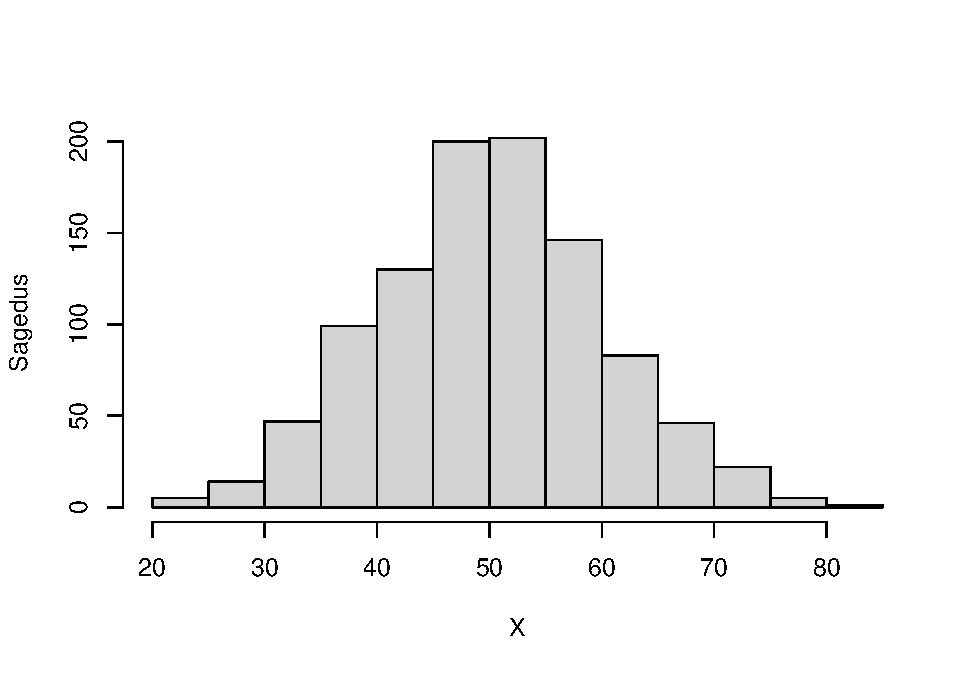
\includegraphics[keepaspectratio]{_main_files/figure-latex/unnamed-chunk-26-1.pdf}}
\caption{\label{fig:unnamed-chunk-26}Histogramm}
\end{figure}

\subsubsection{Sageduste arvutamine}\label{sageduste-arvutamine}

Tulpdiagrammile võib eelnevalt välja arvutada antud sagedused. Selleks saab kasutada funktsiooni \texttt{cut()}, mis vajab rühmade piire sisendiks ning seejärel saab juba funktsiooniga \texttt{table()} loendada kokku iga rühma liikmete arvu.

\begin{Shaded}
\begin{Highlighting}[]
\CommentTok{\# Samasuguse tulemuse saab ka, kui jaotada rühmadesse funktsioonidega cut ja table}
\FunctionTok{barplot}\NormalTok{(tmp }\OtherTok{\textless{}{-}} \FunctionTok{table}\NormalTok{(}\FunctionTok{cut}\NormalTok{(andmed, piirid}\SpecialCharTok{$}\NormalTok{breaks)), }
 \AttributeTok{ylim =} \FunctionTok{c}\NormalTok{(}\DecValTok{0}\NormalTok{, }\FunctionTok{max}\NormalTok{(tmp) }\SpecialCharTok{+} \DecValTok{5}\NormalTok{), }\AttributeTok{ylab=}\StringTok{"Sagedus"}\NormalTok{, }\AttributeTok{xlab =} \StringTok{"X"}\NormalTok{,}
 \AttributeTok{space =} \DecValTok{0}
\NormalTok{)}
\end{Highlighting}
\end{Shaded}

\begin{figure}
\centering
\pandocbounded{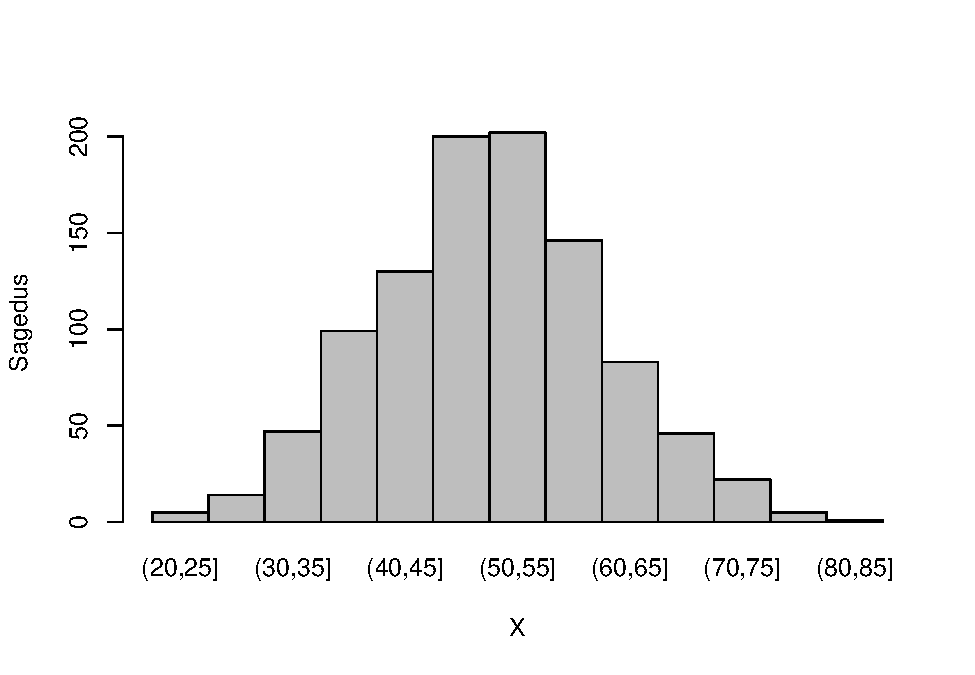
\includegraphics[keepaspectratio]{_main_files/figure-latex/unnamed-chunk-27-1.pdf}}
\caption{\label{fig:unnamed-chunk-27}Tulpdiagramm}
\end{figure}

\subsection{Exceli keskkonnas:}\label{exceli-keskkonnas}

\subsubsection{Histogramm}\label{histogramm-2}

Histogrammi loomiseks Excelis peab andmed esmalt sisestama tabelisse ja seejärel kasutama selle jaoks sobivat tööriista.

\begin{enumerate}
\def\labelenumi{\arabic{enumi}.}
\tightlist
\item
  Sisesta pideva tunnuse väärtused Exceli tabelisse.
\item
  Vali need lahtrid, kuhu soovid luua histogrammi.
\item
  Mine menüüsse ``Lisa'' ja vali ``Diagramm''.
\item
  Vali ``Histogramm'' ja klikka ``OK''.
\item
  Seejärel on võimalik vormindada telje suvandeid, millega määratakse rühmade (MS Exceli keskkonnas nimetusega ``salv'') parameetrid.
\end{enumerate}

\subsubsection{Sageduste arvutamine}\label{sageduste-arvutamine-1}

MS Exceli funktsioon \texttt{FREQUENCY} võimaldab kasutajatel määrata, kui sageli väärtused esinevad teatud väärtusvahemikes. See funktsioon sobib hästi suurte andmekogumite analüüsimiseks, et mõista andmete jaotust ilma iga üksiku väärtuse manuaalse üle vaatamiseta.

Enne \texttt{FREQUENCY} funktsiooni kasutamist peate määrama rühmade vahemike piirid, millesse soovite oma andmed jaotada. Need piirid tuleks sisestada eraldi veergu Exceli töölehel. Näiteks, kui soovite analüüsida testitulemusi vahemikus 0-100, võite määrata piirid 0, 20, 40, 60, 80, 100.

\begin{enumerate}
\def\labelenumi{\arabic{enumi}.}
\tightlist
\item
  \textbf{Andmete ja piiride sisestamine:}
\end{enumerate}

\begin{itemize}
\tightlist
\item
  Sisestage oma andmekogum ühte veergu (nt A2:A101).
\item
  Sisestage vahemike piirid teise veergu (nt B2:B7, eeldades, et esitasite näiteks eelmises punktis toodud piirid).
\end{itemize}

\begin{enumerate}
\def\labelenumi{\arabic{enumi}.}
\setcounter{enumi}{1}
\tightlist
\item
  \textbf{Funktsiooni rakendamine:}
\end{enumerate}

\begin{itemize}
\tightlist
\item
  Valige tühi ala, kuhu soovite tulemused väljastada. Sellel peaks olema sama palju lahtrid kui määratletud vahemike piire. Kui teil on 6 piiri, valige 6 lahtrit vertikaalselt.
\item
  Sisestage \texttt{FREQUENCY} funktsioon. Kuna \texttt{FREQUENCY} on massiivifunktsioon, tuleb see sisestada massiivivalemiga. Algusesse minev andmevahemik on teie andmekogum ja teine vahemik on teie vahemike piirid.
  Näiteks: \texttt{=FREQUENCY(A2:A101,\ B2:B7)}
\item
  Pärast funktsiooni sisestamist lõpetage sisestus, vajutades \textbf{Ctrl+Shift+Enter}. Excel käitab nüüd \texttt{FREQUENCY} funktsiooni massiivina ja täidab valitud lahtrid andmete sagedustega, mis vastavad määratud vahemikele.
\end{itemize}

\chapter{Karakteristikud}\label{karakteristikud}

Statistilised karakteristikud on kvantitatiivsed või kvalitatiivsed omadused, mis kirjeldavad ja iseloomustavad andmekogumeid või andmete jaotusi. Neid kasutatakse andmete kokkuvõtlikuks esitamiseks, et saada arusaam andmete üldisest käitumisest, trendidest ja omadustest. Statistilised karakteristikud võimaldavad teha järeldusi kogu populatsiooni kohta, analüüsides selleks valimit. Peamised statistilised karakteristikud jagunevad kaheks suureks rühmaks: keskmise ja hajuvuse karakteristikud.

Juhuslik suurus on täielikult kirjeldatud üldkogumi jaotus- või tihedusfunktsiooniga (jaotusega). Juhusliku suuruse iseloomustamiseks teatud aspektist kasutatakse erinevaid arvkarakteristikuid. Neist tähtsaim on \textbf{keskväärtus} ehk matemaatiline ootus, mida tähistatakse EX ja mis on defineeritud järgnevalt.

Pideva juhusliku suuruse korral:
\[EX = \sum_{-\infty}^{\infty} x \cdot f(x) dx\]

Diskreetse juhusliku suuruse korral:
\[EX = \sum_{i=1}^{n} x_i \cdot p_i\]

\section{Keskmised}\label{keskmised}

\subsection{Aritmeetiline keskmine}\label{aritmeetiline-keskmine}

Juhusliku suuruse jaotusseadus on uurijale enamasti teadmata. Seetõttu kasutatakse üldkogumi karakteristikute hindamiseks valimi vastavaid karakteristikuid. Üldkogumi keskväärtusele vastab valimi aritmeetiline keskmine, mida tähistatakse ülakriipsuga vastava muutuja kohal \(\bar x\) ja arvutatakse järgnevalt.

\[ \bar x=\frac{1}{N}\sum_{i=1}^{k}n_i \cdot x_i \]

Kus \(x_{i}\) on iga andmehulga liige ning \(n\) on andmehulga suurus.

\textbf{R keskkonnas:}

\begin{Shaded}
\begin{Highlighting}[]
\CommentTok{\# Näide, kus andme\_vektor on vektor numbrilistest väärtustest}
\CommentTok{\# Tunnusest arvutatakse keskmine:}
\FunctionTok{mean}\NormalTok{(andme\_vektor)}
\end{Highlighting}
\end{Shaded}

\begin{verbatim}
## [1] 23,13987
\end{verbatim}

\textbf{Exceli keskkonnas:}

\begin{Shaded}
\begin{Highlighting}[]
\NormalTok{=MEAN(andmeplokk)}
\end{Highlighting}
\end{Shaded}

\subsection{Ruutkeskmine}\label{ruutkeskmine}

Ruutkeskmine on üks keskmise leidmise meetoditest, mis annab ülevaate andmehulgast ning aitab mõõta andmete hajuvust. Ruutkeskmise leidmiseks tuleb iga andmehulga liige ruutu võtta, seejärel leida nende aritmeetiline keskmine ning võtta sellest ruutjuur. Matemaatiliselt väljendatuna on ruutkeskmine järgmine:

\[ \bar x_{ruut}=\sqrt{\frac{1}{N}\sum_{i=1}^{k}n_i \cdot x_i^2} \]

Kus \(x_{i}\) on iga andmehulga liige ning \(n\) on andmehulga suurus.

Metsanduses on ruutkeskmine kasutusel keskmise diameetri arvutamisel.

\textbf{R keskkonnas:}

\begin{Shaded}
\begin{Highlighting}[]
\CommentTok{\# Tunnusest arvutatakse ruut ning keskmisest võetakse ruutjuur:}
\FunctionTok{sqrt}\NormalTok{(}\FunctionTok{mean}\NormalTok{(andme\_vektor}\SpecialCharTok{\^{}}\DecValTok{2}\NormalTok{))}
\end{Highlighting}
\end{Shaded}

\begin{verbatim}
## [1] 23,67037
\end{verbatim}

\textbf{Exceli keskkonnas:}

\begin{Shaded}
\begin{Highlighting}[]
\NormalTok{=SQRT(MEAN(andmeplokk\^{}2))}
\end{Highlighting}
\end{Shaded}

\subsection{Geomeetriline keskmine}\label{geomeetriline-keskmine}

Geomeetriline keskmine on matemaatiline keskmise arvutamise meetod, mis leitakse korrutades kõik antud arvud omavahel ning võttes sellejärel nende arvude geomeetriline keskmise. Geomeetrilise keskmise leidmiseks kasutatakse valem:

Geomeetriline keskmine \(\bar x_{geom}\) on antud valemiga:

\[\bar x_{geom}=\exp \biggl( \frac{1}{N}\sum_{i=n}^k n_i \cdot \ln(x_i) \biggr) \]

kus:

\begin{itemize}
\tightlist
\item
  \(n\) on arvude kogus
\item
  \(x_1, x_2, \ldots, x_n\) on positiivsed arvud
\end{itemize}

\textbf{R keskkonnas:}

\begin{Shaded}
\begin{Highlighting}[]
\CommentTok{\# Tunnusest arvutatakse logaritm ning keskmisest võetakse exponent:}
\FunctionTok{exp}\NormalTok{(}\FunctionTok{mean}\NormalTok{(}\FunctionTok{log}\NormalTok{(andme\_vektor)))}
\end{Highlighting}
\end{Shaded}

\begin{verbatim}
## [1] 22,61406
\end{verbatim}

\textbf{Exceli keskkonnas:}

\begin{Shaded}
\begin{Highlighting}[]
\NormalTok{=GEOMEAN(andmeplokk)}
\end{Highlighting}
\end{Shaded}

\subsection{Harmooniline keskmine}\label{harmooniline-keskmine}

Harmooniline keskmine on statistiline mõõde, mis arvutatakse jagades arvude hulk nende vastandväärtuste summa järgi. Harmooniline keskmine on erinev aritmeetilisest ja geomeetrilisest keskmisest ning seda kasutatakse eelkõige siis, kui on vaja leida keskmine, mis arvestab vastandväärtusi või suhtarve.

Harmoonilist keskmist kasutatakse sageli olukordades, kus on vaja arvutada keskmine mingis suhtarvulises kontekstis, näiteks kiiruste, ajade või muude vastandväärtustega seotud suuruste puhul. Näiteks võib harmooniline keskmine kiirus olla kasulik, kui on vaja arvutada keskmine kiirus teepikkuse ja sõiduaegadega seotud olukorras.

Harmoonilist keskmist arvutatakse valemiga:
\[\bar x_{harm} = \frac{N}{\sum_{i=1}^k n_i / x_i},\]
kus \(x_{1}, x_{2}, \ldots, x_{n}\) on arvude hulk, mille harmoonilist keskmist soovitakse leida ning \(n\) on arvude hulga suurus.

\textbf{R keskkonnas:}

\begin{Shaded}
\begin{Highlighting}[]
\CommentTok{\# Tunnuse pöördväärtuse keskmisest võetakse pöördväärtus:}
\DecValTok{1}\SpecialCharTok{/}\FunctionTok{mean}\NormalTok{(}\DecValTok{1}\SpecialCharTok{/}\NormalTok{andme\_vektor)}
\end{Highlighting}
\end{Shaded}

\begin{verbatim}
## [1] 22,09974
\end{verbatim}

\textbf{Exceli keskkonnas:}

\begin{Shaded}
\begin{Highlighting}[]
\NormalTok{=HARMEAN(andmeplokk)}
\end{Highlighting}
\end{Shaded}

\section{Mediaan}\label{mediaan}

Mediaan väärtus, mis jagab andmed kaheks võrdselt suureks pooleks. See ei sõltu ekstreemsetest väärtustest ega hajutatud andmetest.

Mediaani arvutamine:

\begin{Shaded}
\begin{Highlighting}[]
\FunctionTok{median}\NormalTok{(andme\_vektor)}
\end{Highlighting}
\end{Shaded}

\begin{verbatim}
## [1] 22,8
\end{verbatim}

Exceli keskkonnas:

\begin{Shaded}
\begin{Highlighting}[]
\NormalTok{=MEDIAN(andmeplokk)}
\end{Highlighting}
\end{Shaded}

\section{Kvantiilid}\label{kvantiilid}

Juhusliku suuruse p-kvantiiliks (0 \textless{} p \textless{} 1) nimetatakse sellist juhusliku suuruse väärtust xp, millest väiksemate väärtuste esinemise tõenäosus on p:

\[ P (X < x_p) = p \]

Teatud kvantiilide jaoks kasutatakse erinimetusi:

\begin{itemize}
\tightlist
\item
  \(x_{0,50}\) -- mediaan, tähistatakse ka Me;
\item
  \(x_{0,25}\) -- alumine kvartiil;
\item
  \(x_{0,75}\) -- ülemine kvartiil;
\item
  \(x_{0,10}\) -- alumine detsiil;
\item
  \(x_{0,9}\) -- ülemine detsiil;
\item
  \(x_{0,01}\) -- alumine protsentiil;
\item
  \(x_{0,99}\) -- ülemine protsentiil.
\end{itemize}

Enamkasutatavam kvantiil on \textbf{mediaan}, mida võib pidada (nagu keskväärtustki) juhusliku suuruse tsentriks. Mediaan on juhusliku suuruse selline väärtus, millest nii väiksemate kui ka suuremate väärtuste esinemise tõenäosus on 0,5. Mediaan iseloomustab juhusliku suuruse asendi poolest keskmist väärtust.
Kui on teada juhusliku suuruse jaotusfunktsioon F(x), siis saab juhusliku suuruse kvantiili xp arvutada kui jaotusfunktsiooni pöördfunktsiooni, sest kvantiili definitsioonist tuleneb F(xp) = p.~Juhul kui on tegemist vaatlusandmestikuga, saab kvantiile ligikaudu hinnata empiiriliselt jaotusfunktsiooni graafikult.

Mediaani arvutamine:

\textbf{R keskkonnas:}

\begin{Shaded}
\begin{Highlighting}[]
\FunctionTok{median}\NormalTok{(andme\_vektor)}
\end{Highlighting}
\end{Shaded}

\begin{verbatim}
## [1] 22,8
\end{verbatim}

\textbf{Exceli keskkonnas:}

\begin{Shaded}
\begin{Highlighting}[]
\NormalTok{=MEDIAN(andmeplokk)}
\end{Highlighting}
\end{Shaded}

\chapter{Jaotusfunktsioonid}\label{jaotusfunktsioonid}

Teoreetilisi jaotusi kasutatakse hüpoteeside testimisel statistilistes analüüsides selleks, et teha kindlaks, kas vaatlusandmete hajuvus on juhuslik või on olemas mingi muster või seos. Oluline on märkida, et enamik statistilisi teste eeldab teatud jaotuse tundmist, mille põhjal tehakse järeldusi populatsiooni kohta.

Kõige tuntum teoreetiline jaotus on normaaljaotus, mis on sümmeetriline kõver ning annab tihti paljudele looduslikele nähtustele lähedase jaotuse. Normaaljaotus on oluline paljudes statistilistes testimistes, näiteks t-testis või ANOVA analüüsis. Kui andmed järgivad normaaljaotust, saab kasutada erinevaid statistilisi meetodeid.

Lisaks normaaljaotusele on olulised ka teised jaotused, nagu näiteks binoomjaotus (kasutatakse binomiaalsete katsete puhul), eksponentiaaljaotus (kasutatakse elupikkuste analüüsimisel) ja Poissoni jaotus (kasutatakse haruldaste sündmuste analüüsimisel).

Hüpoteeside testimisel võrreldakse empiirilisi andmeid teoreetiliste jaotustega, et teha järeldusi populatsiooni kohta. Näiteks võib uurida, kas kahe rühma keskmiste vahel on oluline erinevus või kas mingi seos on juhuslik või mitte. Sellisel juhul kasutatakse statistilisi teste, et hinnata, kas tulemus võib olla juhuslik või on tõenäoliselt tingitud tegelikust mõjust või seosest.

\section{Hüpotees}\label{huxfcpotees}

Hüpotees on statistikas väide või eeldus, millele toetudes teostatakse uuringuid, analüüsi või katseid. Hüpotees võib olla kas uurija poolt esitatud eeldus, mida on vaja tõestada või ümber lükata või juba olemasolev teooria, mida soovitakse kontrollida. Statistilises analüüsis on nullhüpotees (tähistatud kui \(H_0\)) teoreetiline väide, mis tavaliselt väljendab, et mingisugust mõju, erinevust või seost uuritavate muutujate vahel ei ole. See on baashüpotees, mida testitakse statistiliste meetodite abil, et hinnata, kas kogutud andmed annavad piisavalt tõendeid nullhüpoteesi tagasilükkamiseks või mitte.

Statistilise testi põhiprotsess nullhüpoteesi kontekstis hõlmab järgmisi samme:

\begin{enumerate}
\def\labelenumi{\arabic{enumi}.}
\tightlist
\item
  \textbf{Nullhüpoteesi ja alternatiivhüpoteesi (\(H_a\)) sõnastamine}: Alternatiivhüpotees väljendab uuritava efekti, erinevuse või seose olemasolu. Hüpoteesid võib jagada kaheks:
\end{enumerate}

\begin{itemize}
\item
  \textbf{Nullhüpotees (H0):} Nullhüpotees esitab eelduse, et mingit seost või erinevust populatsiooni omaduste vahel ei ole. Näiteks, kui soovid uurida, kas kahe rühma keskmised on erinevad, siis nullhüpotees võib olla, et keskmised ei erine.
\item
  \textbf{Alternatiivhüpotees (H1 või Ha):} Alternatiivhüpotees esitab vastupidise väite nullhüpoteesile. Kas nullhüpoteesi ei ole põhjust uskuda või kas kehtib eeldus, mille kohaselt on mingi seos olemas. jätkates eelnevat näidet, alternatiivhüpotees võib olla, et kahe rühma keskmised on erinevad.
\end{itemize}

\begin{enumerate}
\def\labelenumi{\arabic{enumi}.}
\setcounter{enumi}{1}
\item
  \textbf{Taseme (\(\alpha\)) valimine}: See on tõenäosus, millega ollakse valmis aktsepteerima valepositiivset tulemust (tüüp I viga), ehk olukorda, kus nullhüpoteesi lükatakse tagasi, kuigi see on tegelikult tõene. Tavaliselt kasutatakse 0.05 või 5\% tasemet.
\item
  \textbf{Sobiva statistilise testi valik} sõltuvalt andmete omadustest ja uurimisküsimusest.
\item
  \textbf{Teststatistiku arvutamine ja P-väärtuse leidmine}: Teststatistiku väärtus näitab, kui tõenäoline on saadud või veelgi äärmuslikum tulemus, eeldusel, et nullhüpotees on tõene. P-väärtus väljendab seda tõenäosust.
\item
  \textbf{Otsuse tegemine}: Kui P-väärtus on väiksem kui eelnevalt valitud tase \(\alpha\), siis lükatakse nullhüpotees tagasi. See tähendab, et leiti statistiliselt oluline erinevus. Kui P-väärtus on suurem kui \(\alpha\), siis nullhüpoteesi ei lükata tagasi.
\end{enumerate}

Tuleb arvestada, et nullhüpoteesi ei saa ``tõestada'', kuna statistiliste testidega ei saa nullhüpoteesi tõestada samamoodi, nagu matemaatikas võidakse tõestada väiteid. Selle asemel saab statistiliste testide abil hinnata, kas on piisavalt tõendeid nullhüpoteesi tagasilükkamiseks. Kui testi tulemus näitab, et andmed on nullhüpoteesiga vastuolus, siis võidakse nullhüpotees tagasi lükata. Kui aga testi tulemus ei näita olulist vastuolu nullhüpoteesiga, siis ei lükata nullhüpoteesi tagasi. Siiski, see ei tähenda, et nullhüpotees oleks ``tõestatud''; pigem öeldakse, et ei leitud piisavalt tõendeid nullhüpoteesi ümberlükkamiseks. Oluline on mõista, et nullhüpoteesi mitte-tagasilükkamine ei tõesta selle paikapidavust. See viitab lihtsalt sellele, et andmed ei andnud piisavalt alust nullhüpoteesi ümber lükata. Samuti on oluline meeles pidada, et statistiliste testide tulemused annavad ainult tõenäosusliku hinnangu ning need tuleb alati panna laiemasse konteksti koos teiste tõendite ja teadmistega valdkonnast.

\section{Jaotusfunktsioon}\label{jaotusfunktsioon}

Jaotusfunktsioon on viis näidata, kui tõenäoline on, et mingi arv (mida me nimetame muutujaks) on väiksem või võrdne kindla arvuga x. See aitab meil mõista, kuidas arvud (või muutujad) ühes grupis paiknevad või jaotuvad, näiteks kui me tahame teada, kui tõenäoline on, et metsa pindala on teatud suurusega või väiksem.

Jaotusfunktsiooni olulised omadused on:

\begin{enumerate}
\def\labelenumi{\arabic{enumi}.}
\item
  Vahemik: jaotusfunktsioon võtab väärtuseid 0 ja 1 vahemikus, mis tähendab, et tõenäosus on alati selles vahemikus.
\item
  Mittelangus: jaotusfunktsioon ei kasva kunagi tagurpidi; see liigub alati kas võrdse kõrguse juurde või kõrgemale.
\item
  Ühekordsus: Ükskõik millised on väärtused, jaotusfunktsiooni koguulatus on alati 1.
\end{enumerate}

Jaotusfunktsiooni abil saame lahendada paljusid statistilisi ülesandeid. See aitab meil leida näiteks keskmisi väärtusi, hajuvust (ehk kui laiali arvud on jaotunud), tõenäosusi (kui tõenäoline on mingi sündmus), ja isegi määrata arvude jaotuse erinevaid tasemeid. See tähendab, et jaotusfunktsioon on tööriist, mis aitab meil mõista, kuidas andmed käituvad, ja teha selle põhjal täpseid otsuseid või järeldusi.

Näide R-is jaotusfunktsiooni graafiliseks esitamiseks:

Käsk \texttt{plot(ecdf(x),\ verticals\ =\ TRUE,\ main\ =\ "",\ xlab\ =\ "x",\ ylab\ =\ "F(x)",\ lwd\ =\ 2)} R keeles genereerib empirilise kumulatiivse jaotusfunktsiooni (ECDF) graafiku muutuja \texttt{x} andmetele. ECDF on kasulik statistiline tööriist, mis näitab iga andmepunkti või väiksemat väärtust omavate andmepunktide suhtelist osakaalu andmestikus. Allpool on toodud, kuidas see käsk töötab ja mida see illustreerib:

\begin{itemize}
\item
  \textbf{\texttt{ecdf(x)}:} Loob empirilise kumulatiivse jaotusfunktsiooni andmestikust \texttt{x}. ECDF on funktsioon, mille väärtus igas punktis \(x\) on andmepunktide osakaal, mis on väiksem või võrdne \(x\)-ga. See on kasulik andmete jaotuse visualiseerimiseks ja andmepunktide vaheliste suhete mõistmiseks.
\item
  \textbf{\texttt{plot()}:} Joonistab ECDF graafiku. Selles kontekstis:
\item
  \texttt{verticals\ =\ TRUE} määrab, et graafikule joonistatakse vertikaalsed jooned iga hüppe kohale, mis muudab jaotuse astmed visuaalselt selgemaks.
\item
  \texttt{main\ =\ ""} jätab graafiku pealkirja tühjaks.
\item
  \texttt{xlab\ =\ "x"} ja \texttt{ylab\ =\ "F(x)"} määravad vastavalt x-telje ja y-telje sildid. \texttt{x} tähistab andmepunkte ja \texttt{F(x)} on kumulatiivse jaotusfunktsiooni väärtus, mis näitab andmepunktide suhtelist kumulatiivset osakaalu.
\item
  \texttt{lwd\ =\ 2} määrab joone laiuse, muutes joone graafikul paksemaks ja paremini nähtavaks.
\item
  \textbf{Andmete Jaotus:} ECDF graafik annab intuitiivse ülevaate andmete jaotusest, näidates, kui suur osa andmestikust on alla või võrdne iga võimaliku väärtusega. See on eriti kasulik andmete jaotuse mõistmiseks ilma eeldamata mingit konkreetset jaotustüüpi.
\item
  \textbf{Outlierid ja Andmete Levik:} Graafik võib samuti aidata tuvastada võimalikke väljapoole jäävaid väärtusi (outliereid) ja muid andmete leviku iseärasusi, näiteks kui andmete jaotus ei ole ühtlane.
\end{itemize}

ECDF graafik on väärtuslik tööriist andmete uurimisel, võimaldades kiiresti hinnata andmete jaotuse omadusi ja tuvastada andmete levikuga seotud probleeme.

\begin{Shaded}
\begin{Highlighting}[]
\CommentTok{\# Loome andmestik}
\FunctionTok{set.seed}\NormalTok{(}\DecValTok{123}\NormalTok{)}
\NormalTok{x }\OtherTok{\textless{}{-}} \FunctionTok{rnorm}\NormalTok{(}\DecValTok{1000}\NormalTok{, }\AttributeTok{mean =} \DecValTok{0}\NormalTok{, }\AttributeTok{sd =} \DecValTok{1}\NormalTok{)}

\CommentTok{\# Loome kumulatiivse jaotusfunktsiooni graafiku}
\FunctionTok{plot}\NormalTok{(}\FunctionTok{ecdf}\NormalTok{(x), }\AttributeTok{verticals =} \ConstantTok{TRUE}\NormalTok{, }\AttributeTok{main =} \StringTok{""}\NormalTok{, }\AttributeTok{xlab =} \StringTok{"x"}\NormalTok{, }\AttributeTok{ylab =} \StringTok{"F(x)"}\NormalTok{, }\AttributeTok{lwd =} \DecValTok{2}\NormalTok{)}

\CommentTok{\# Arvutame sama kasutades funktsiooni quantile}
\NormalTok{kv.pos }\OtherTok{\textless{}{-}} \FunctionTok{seq}\NormalTok{(}\DecValTok{0}\NormalTok{, }\DecValTok{1}\NormalTok{, }\AttributeTok{by =} \FloatTok{0.05}\NormalTok{)}
\NormalTok{jf.q }\OtherTok{\textless{}{-}} \FunctionTok{quantile}\NormalTok{(x, }\AttributeTok{probs =}\NormalTok{ kv.pos)}
\FunctionTok{lines}\NormalTok{(jf.q, kv.pos, }\AttributeTok{col =} \DecValTok{2}\NormalTok{, }\AttributeTok{lty =} \DecValTok{2}\NormalTok{, }\AttributeTok{lwd=}\DecValTok{2}\NormalTok{)}

\CommentTok{\# Arvutame andmete sortimise kaudu}
\CommentTok{\# y tunnus on selle suhteline järjekorranumber ehk vahemikul 0 ... 1}
\NormalTok{n }\OtherTok{\textless{}{-}} \FunctionTok{length}\NormalTok{(x)}
\FunctionTok{lines}\NormalTok{(}\FunctionTok{sort}\NormalTok{(x), }\DecValTok{1}\SpecialCharTok{:}\NormalTok{n}\SpecialCharTok{/}\NormalTok{n, }\AttributeTok{col =} \DecValTok{3}\NormalTok{)}
\end{Highlighting}
\end{Shaded}

\begin{figure}
\centering
\pandocbounded{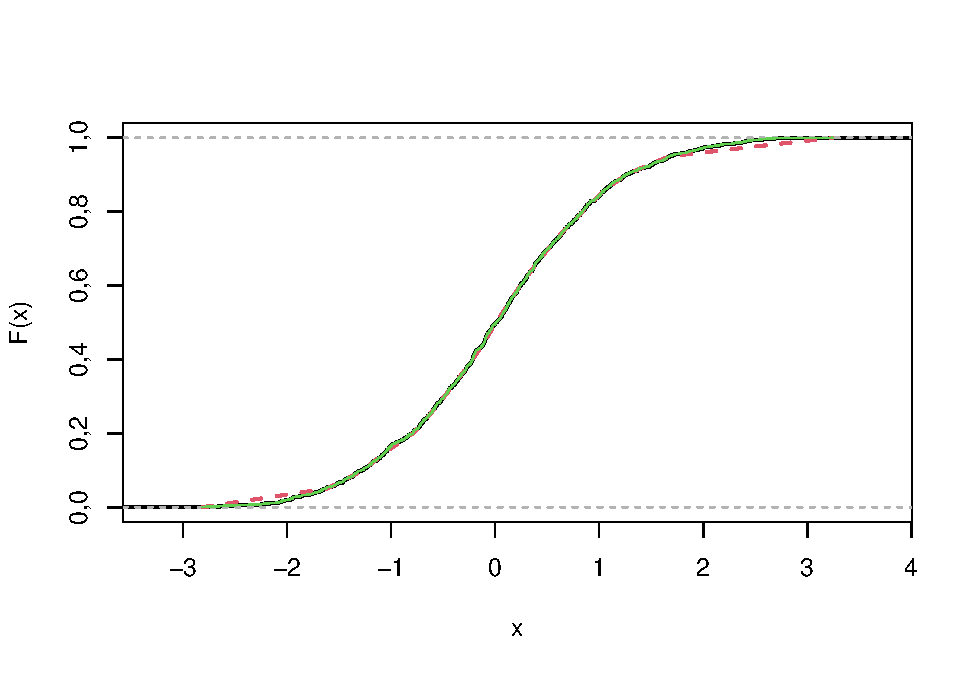
\includegraphics[keepaspectratio]{_main_files/figure-latex/unnamed-chunk-43-1.pdf}}
\caption{\label{fig:unnamed-chunk-43}Empiiriline jaotusfunktsioon erinevate meetoditega}
\end{figure}

Selgitus:

\begin{itemize}
\tightlist
\item
  Loome andmestiku \texttt{x}, kasutades siin normaaljaotuse näidet.
\item
  Joonistame kumulatiivse jaotusfunktsiooni kasutades \texttt{ecdf()} funktsiooni, mis arvutab empiirilise kumulatiivse jaotusfunktsiooni andmestiku põhjal.
\item
  \texttt{plot} funktsiooniga joonistame graafiku x-telje nimetuse (``x'') ja y-telje nimetuse (``F(x)'').
\item
  Arvutame kvantiilid (\texttt{quantile(x,\ probs\ =\ kv.pos)}) ning lisame joonisele tulemuse.
\item
  Järjestame kasvavas järjekorras (\texttt{sort(x)}) ning arvutame selle suhtelise järjekorranumbri (1:n/n)
\end{itemize}

Need on erinevad võimalused arvutada empiirilist jaotusfunktsiooni.

\section{Tihedusfunktsioon}\label{tihedusfunktsioon}

Tihedusfunktsioon on statistikas kasutatav funktsioon, mis kirjeldab tõenäosust, et juhuslik suurus langeb mingisse kindlasse vahemikku. Tihedusfunktsiooni saab kasutada tõenäosusjaotuse (nt normaaljaotus, Bernoulli jaotus jne) karakteriseerimiseks. See näitab, kui tõenäoline on konkreetse väärtuse saamine selle jaotuse järgi.

Tihedusfunktsioon on graphiline joon, mis esitab tõenäosuse jaotuse ühtlase tervikuna. Üksiku väärtuse tõenäosus on antud tihedusfunktsiooni abil vahemikuna, mida funktsioon katab selles punktis. Tavaliselt on tihedusfunktsioon positiivne ja integreerub üle vahemiku 1, mis tähendab, et kõikidele võimalikele väärtustele vastavate tõenäosuste summa on alati 1.

Metsanduses võib tihedusfunktsiooni kasutada näiteks puistu tiheduse jaotuse kirjeldamisel, kus tihedusfunktsioon näitab puude arvu tõenäosust kindlas pindalas. Tihedusfunktsioonide abil saab hinnata erinevaid statistilisi parameetreid nagu keskmine, mediaan, variatsioon jt, ning teha ennustusi ja otsuseid metsaressursi haldamisel ja planeerimisel.

Tihedusfunktsioon (inglise keeles probability density function, lühidalt PDF) on statistikas oluline mõiste, mida kasutatakse tõenäosusjaotuse kirjeldamiseks. Tihedusfunktsioon annab meile informatsiooni selle kohta, kuidas on tõenäosus mingi juhusliku muutuja väärtuse jaotustel. Allpool on toodud mõned olulised statistilised omadused tihedusfunktsiooni kohta:

\index{Integreeruvus}\textbf{Integreeruvus}: tihedusfunktsioon peab olema integreeruv kogu kandva ala suhtes, st selle integraal alates miinimum- kuni maksimumväärtuseni peab olema võrdne ühega. Teisisõnu, kogu võimaliku vaadeldava mahu (nt kogu metsaala, kus uuritakse puude tihedust) peab olema 100\%.

\index{Positiivsus:}\textbf{Positiivsus:} Tihedusfunktsiooni väärtused peavad olema alati positiivsed. See tähendab, et tõenäosus väärtuse sattumiseks konkreetsesse intervalli ei saa olla negatiivne.

\index{Normaliseerumine:}\textbf{Normaliseerumine:} Tihedusfunktsioon peab olema normaliseeritud, mis tähendab, et alati, kui me integreerime tihedusfunktsiooni kogu liinil või tasandil, siis tulemuseks peab olema üks. See tagab, et tihedusfunktsioon annab meile täpse tõenäosuse, et vaadeldav suurus langeb mingisse kindlasse vahemikku.

\index{Mitte-negatiivsus:}\textbf{Mitte-negatiivsus:} Tihedusfunktsioon ei või mitte kunagi võtta negatiivseid väärtusi. See tähendab, et tõenäosus mingi suuruse väärtuse jaoks on alati null või suurem.

\index{Tipukoha lokaliseerimine:}\textbf{Tipukoha lokaliseerimine:} Tihedusfunktsiooni tippkoht näitab moodi ehk suurimat tõenäosust mingi väärtuse saamiseks. Mood on statistikas näitaja, mis näitab, milline väärtus esineb andmehulgas kõige sagedamini ehk mis väärtusega esineb andmehulkade hulgas enim kordi. Mood on üks keskmiste näitajate tüüpe, mis aitab anda ülevaadet andmete esinemissagedusest konkreetse väärtuse juures.

Need omadused on olulised tihedusfunktsiooni mõistmisel ja kasutamisel statistilistes analüüsides, sealhulgas metsanduses, kus tihedusfunktsiooni abil saab kirjeldada erinevaid muutujaid nagu puu tihedus, metsa elujõulisus jne.

Näide R-i koodist, mis genereerib normaaljaotuse tihedusfunktsiooni graafiku:

\begin{Shaded}
\begin{Highlighting}[]
\CommentTok{\# Genereerime juhuslikud andmed normaaljaotusest}

\CommentTok{\# Koostame graafiku}
\FunctionTok{plot}\NormalTok{(df.tul }\OtherTok{\textless{}{-}} \FunctionTok{density}\NormalTok{(x, }\AttributeTok{bw =} \FloatTok{0.3}\NormalTok{), }\AttributeTok{main =} \StringTok{""}\NormalTok{, }\AttributeTok{xlab=}\StringTok{"x"}\NormalTok{, }\AttributeTok{ylab=}\StringTok{"f(x)"}\NormalTok{)}
\CommentTok{\# leiame mood väärtuse: x väärtus, mille y on maksimaalne}
\FunctionTok{abline}\NormalTok{(}\AttributeTok{v =}\NormalTok{ df.tul}\SpecialCharTok{$}\NormalTok{x[}\FunctionTok{which}\NormalTok{(df.tul}\SpecialCharTok{$}\NormalTok{y }\SpecialCharTok{==} \FunctionTok{max}\NormalTok{(df.tul}\SpecialCharTok{$}\NormalTok{y))], }\AttributeTok{col =} \DecValTok{2}\NormalTok{)}
\end{Highlighting}
\end{Shaded}

\begin{figure}
\centering
\pandocbounded{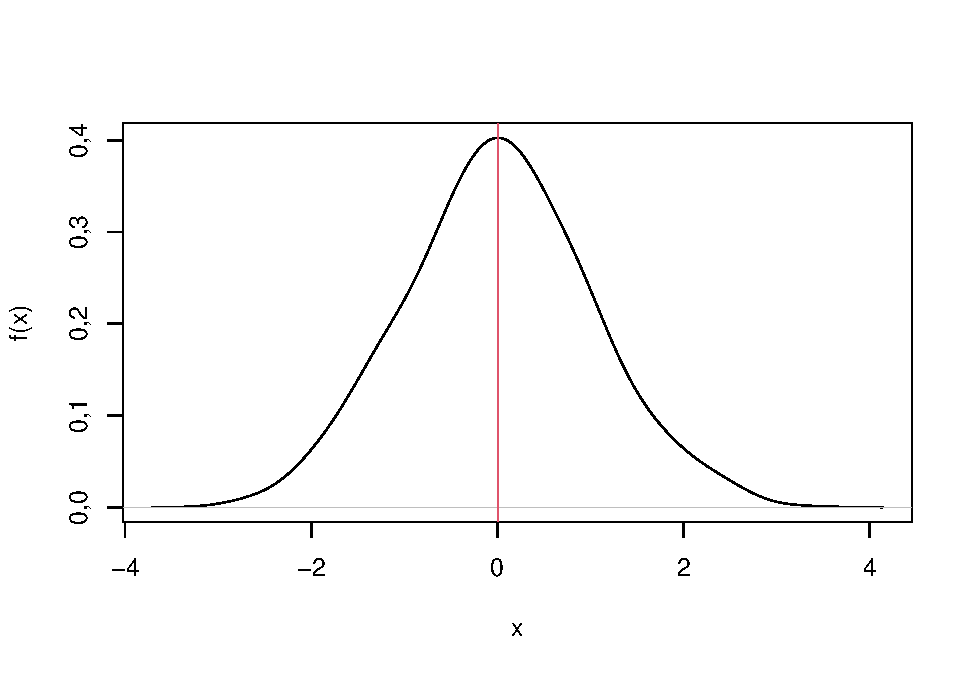
\includegraphics[keepaspectratio]{_main_files/figure-latex/unnamed-chunk-44-1.pdf}}
\caption{\label{fig:unnamed-chunk-44}Empiiriline tihedusfunktsioon.}
\end{figure}

See kood genereerib normaaljaotuse tihedusfunktsiooni graafiku, kus x-teljel on andmete väärtused ja y-teljel tihedusfunktsiooni väärtused. Graafik peaks näitama tüüpilist kausitaolist kõverust normaaljaotuse puhul. Vajadusel saab koodi muuta, et kohandada graafiku väljanägemist ja andmete genereerimise parameetreid vastavalt vajadusele.

\section{Normaaljaotus}\label{normaaljaotus}

Normaaljaotus ehk Gaussi jaotus on tõenäosusjaotus, mida iseloomustab sümmeetriline kellakujuline tõenäosustiheduse graafik ning parameetrid keskväärtus (mean) ja standardhälve (standard deviation).

Normaaljaotuse tõenäosustiheduse funktsioon on defineeritud järgmiselt:
\[ f(x) = \frac{1}{\sigma \sqrt{2\pi}} e^{-\frac{(x - \mu)^2}{2\sigma^2}}, \]
kus:
- \(f(x)\) on tõenäosustiheduse funktsioon;
- \(\sigma\) on standardhälve, mis näitab, kui hajus on andmete hulk;
- \(\mu\) on keskväärtus, mis näitab andmete keskmist väärtust;
- \(e\) on Euleri arv, kus \(e \approx 2.71828\).

Normaaljaotuse oluline omadus on see, et suure hulga juhuslike sündmuste kogum tulemusena on nende keskmine jaotunud normaalselt. Samuti on oluline märkida, et normaaljaotus on sümmeetriline ning selle standardiseeritud kuju \(N(0,1)\) on standardnormaaljaotus, mille keskväärtus on 0 ja standardhälve on 1.

Normaaljaotus on laialdaselt kasutatav statistikas erinevate nähtuste kirjeldamisel ning analüüsimisel, sh metsanduses, kus seda võib kasutada näiteks puude kõrguse või läbimõõdu jaotuste modelleerimisel ning hindamisel.

Normaaljaotust kasutatakse paljudes erinevates valdkondades, sealhulgas statistikas, majanduses ja teaduses. Metsanduses võib normaaljaotust kasutada näiteks metsa populatsiooni omaduste hindamiseks või metsanduslike nähtuste, nagu puude kõrgus või läbimõõt, jaotuse kirjeldamiseks.

Siin on mõned põhjused, miks normaaljaotust kasutatakse:

\begin{itemize}
\item
  Andmete kirjeldamine: Normaaljaotust kasutatakse tihti andmete kirjeldamiseks, kuna paljud looduslikud ja inimtegevuse tulemusena tekkinud nähtused järgivad sarnast jaotusmustrit. Normaaljaotus võimaldab kompaktselt kirjeldada, kuidas andmed on keskmise ümber hajunud.
\item
  Statistiliste meetodite rakendamine: Paljud statistilised meetodid eeldavad, et andmed järgivad normaaljaotust. Näiteks on t-test ja ANOVA analüüsid välja töötatud eeldusel, et andmed on normaalselt jaotunud. Seega aitab normaaljaotuse eeldamine tagada statistiliste meetodite usaldusväärsuse.
\item
  Prognoosimine ja ennustamine: Normaljaotuse kasutamine võimaldab prognoosida tulevasi väärtusi ja sündmusi, eeldusel, et andmed järgivad seda jaotust. See võib aidata metsanduses näiteks prognoosida metsaressursi kasvu või hindamist.
\end{itemize}

Kokkuvõtvalt võib öelda, et normaaljaotuse kasutamine aitab andmeid paremini mõista, analüüsida ja tõlgendada, ning tagada, et nende tehtud järeldused oleksid usaldusväärsed ja põhineksid adekvaatsetel statistilistel mudelitel.

R-is on järgnevad normaaljaotuse funktsioonid:

\begin{itemize}
\tightlist
\item
  \texttt{pnorm()}:

  \begin{itemize}
  \tightlist
  \item
    Kirjeldus: funktsioon \texttt{pnorm()} arvutab normaaljaotuse kumulatiivse tõenäosuse.
  \item
    Kasutamine: \texttt{pnorm(x,\ mean,\ sd)} kus x on punkt, mille tõenäosust soovite arvutada, mean on normaaljaotuse keskmine ja sd on standardhälve.
  \item
    Näide: \texttt{pnorm(1.96,\ 0,\ 1)} annab tõenäosuse, et normaaljaotuse väärtus on väiksem või võrdne 1,96.
  \end{itemize}
\item
  \texttt{dnorm()}:

  \begin{itemize}
  \tightlist
  \item
    Kirjeldus: funktsioon \texttt{dnorm()} arvutab normaaljaotuse tõenäosustiheduse funktsiooni.
  \item
    Kasutamine: \texttt{dnorm(x,\ mean,\ sd)} kus x on punkt, mille tõenäosustihedust soovite arvutada, mean on normaaljaotuse keskmine ja sd on standardhälve.
  \item
    Näide: \texttt{dnorm(1.96,\ 0,\ 1)} annab normaaljaotuse tõenäosustihedust väärtuses 1,96.
  \end{itemize}
\item
  \texttt{qnorm()}:

  \begin{itemize}
  \tightlist
  \item
    Kirjeldus: \texttt{qnorm()} funktsioon arvutab normaaljaotuse kvantiili väärtuse.
  \item
    Kasutamine: \texttt{qnorm(p,\ mean,\ sd)} kus p on soovitud kvantiil, mean on normaaljaotuse keskmine ja sd on standardhälve.
  \item
    Näide: \texttt{qnorm(0.975,\ 0,\ 1)} annab normaaljaotuse ülemise kvantiili 0,975 väärtuse.
  \end{itemize}
\end{itemize}

MS Exceli keskkonnas normaaljaotusega seotud arvutuste tegemiseks saab kasutada järgmisi funktsioone:

\begin{itemize}
\tightlist
\item
  \texttt{NORM.DIST()}:

  \begin{itemize}
  \tightlist
  \item
    Kirjeldus: \texttt{NORM.DIST()} funktsioon arvutab normaaljaotuse tõenäosustiheduse või kumulatiivse tõenäosuse.
  \item
    Kasutamine: NORM.DIST(x, keskmine, standardhälve, kumulatiiv) kus x on punkt, mille tõenäosustihedust või kumulatiivset tõenäosust soovite arvutada, keskmine on jaotuse keskmine, standardhälve on jaotuse standardhälve, ja kumulatiiv on loogiline väärtus, mis määrab, kas funktsioon tagastab tiheduse (FALSE) või kumulatiivse tõenäosuse (TRUE).
  \item
    Näide: NORM.DIST(1,96; 0; 1; TRUE) annab tõenäosuse, et normaaljaotuse väärtus on väiksem või võrdne 1.96.
  \end{itemize}
\item
  \texttt{NORM.S.DIST()}:

  \begin{itemize}
  \tightlist
  \item
    Kirjeldus: \texttt{NORM.S.DIST()} funktsioon arvutab standardnormaaljaotuse tõenäosustiheduse või kumulatiivse tõenäosuse.
  \item
    Kasutamine: NORM.S.DIST(z; kumulatiiv) kus z on punkt standardnormaaljaotuses, mille tõenäosustihedust või kumulatiivset tõenäosust soovite arvutada, ja kumulatiiv on loogiline väärtus, mis määrab, kas funktsioon tagastab tiheduse (FALSE) või kumulatiivse tõenäosuse (TRUE).
  \item
    Näide: NORM.S.DIST(1,96; TRUE) annab tõenäosuse, et standardnormaaljaotuse väärtus on väiksem või võrdne 1.96.
  \end{itemize}
\item
  \texttt{NORM.INV()}:

  \begin{itemize}
  \tightlist
  \item
    Kirjeldus: \texttt{NORM.INV()} funktsioon arvutab normaaljaotuse kvantiili antud tõenäosuse jaoks.
  \item
    Kasutamine: NORM.INV(tõenäosus, keskmine, standardhälve) kus tõenäosus on kvantiili vastav tõenäosus, keskmine on jaotuse keskmine, ja standardhälve on jaotuse standardhälve.
  \item
    Näide: NORM.INV(0,975; 0; 1) annab normaaljaotuse kvantiili, mis vastab 0.975 tõenäosusele.
  \end{itemize}
\item
  \texttt{NORM.S.INV()}:

  \begin{itemize}
  \tightlist
  \item
    Kirjeldus: \texttt{NORM.S.INV()} funktsioon arvutab standardnormaaljaotuse kvantiili antud tõenäosuse jaoks.
  \item
    Kasutamine: \texttt{NORM.S.INV(tõenäosus)} kus tõenäosus on kvantiili vastav tõenäosus standardnormaaljaotuses.
  \item
    Näide: \texttt{NORM.S.INV(0,975)} annab standardnormaaljaotuse kvantiili, mis vastab 0.975 tõenäosusele.
  \end{itemize}
\end{itemize}

\section{T-jaotus}\label{t-jaotus}

T-jaotus ehk Studenti t-jaotus on statistiline jaotus, mis on nimetatud selle looja William Sealy Gosseti (Studendi) järgi. T-jaotust kasutatakse hinnangute tegemiseks populatsiooni keskmise või vahe tegeliku väärtuse kohta, kui meil on vaid valimi keskmine ja standardhälve ning väike valimi suurus.

T-jaotuse tihedusfunktsioon sõltub vabadusastmetest, mida tähistatakse tähisega n-1, kus n on valimi suurus. Mida suurem on vabadusastmete arv, seda lähemale liigub t-jaotuse kumerus standardnormaaljaotusele. T-jaotust kasutatakse sageli siis, kui populatsiooni standardhälve on teadmata ja valimi suurus on alla 30.

T-jaotus on oluline tööriist hüpoteeside testimisel ja usaldusintervallide arvutamisel. Selle abil saame teha järeldusi populatsiooni keskmise kohta isegi siis, kui populatsiooni kohta on vähe teavet. T-jaotust kasutatakse laialdaselt erinevates valdkondades, sealhulgas meditsiinis, majanduses ja loodusteadustes, sealhulgas metsanduses.

t-jaotus on statistikas oluline jaotus, mida kasutatakse tõenäosusteoorias ja hüpoteeside testimisel. T-jaotus sarnaneb normaaljaotusega, kuid erinevalt normaaljaotusest on t-jaotus paindlikum ning sellel on erinev arv vabadusastmeid. T-jaotust kasutatakse peamiselt siis, kui uuritav valim on väike ning populatsiooni standardhälve on teadmata.

Peamised t-jaotuse kasutamise eesmärgid on:

\begin{enumerate}
\def\labelenumi{\arabic{enumi}.}
\item
  Võrdlused: T-jaotust kasutatakse kahe või enama rühma vaheliste erinevuste või keskmiste võrdlemiseks. Näiteks võib t-jaotust kasutada selleks, et teha kindlaks, kas kahe erineva metsa keskmine juurdekasv on statistiliselt oluliselt erinev.
\item
  Hüpoteeside testimine: T-jaotust kasutatakse hüpoteeside testimisel, et teha kindlaks, kas uuritava andmestiku tulemused on juhuslikud või kas seal on tõepoolest mingisugune seos või erinevus. Näiteks võib t-jaotust kasutada selleks, et testida, kas metsa uuendamine teatud viisil mõjutab metsa biomassi kasvu.
\item
  Usaldusintervallid: T-jaotust kasutatakse usaldusintervallide arvutamiseks. Usaldusintervall aitab hinnata, kui usaldusväärne on uuritava keskmise või erinevuse hinnang ning kui suured võivad olla võimalikud vead hinnangus.
\end{enumerate}

Kokkuvõttes on t-jaotus oluline tööriist statistilistes analüüsides, eriti kui tegemist on väikese valimi suuruse ja/või teadmata standardhälbe või suurema vabadusastmega. Metsandustudengite jaoks on t-jaotuse mõistmine ja oskuslik kasutamine oluline, kuna see aitab neil teha täpsemaid järeldusi ja otsuseid metsandusega seotud probleemide lahendamisel.

\begin{enumerate}
\def\labelenumi{\arabic{enumi}.}
\tightlist
\item
  \textbf{pt}:
\end{enumerate}

\begin{itemize}
\tightlist
\item
  \textbf{Kirjeldus}: pt funktsioon arvutab t-jaotuse kumulatiivse tõenäosuse.
\item
  \textbf{Kasutamine}: pt(x, df) kus x on punkt, mille tõenäosust soovite arvutada, ja df on vabadusastmete arv.
\item
  \textbf{Näide}: pt(2.26, 10) annab tõenäosuse, et t-jaotuse väärtus on väiksem või võrdne 2.26, kui vabadusastmete arv on 10.
\end{itemize}

\begin{enumerate}
\def\labelenumi{\arabic{enumi}.}
\setcounter{enumi}{1}
\tightlist
\item
  \textbf{dt}:
\end{enumerate}

\begin{itemize}
\tightlist
\item
  \textbf{Kirjeldus}: dt funktsioon arvutab t-jaotuse tõenäosustiheduse funktsiooni.
\item
  \textbf{Kasutamine}: dt(x, df) kus x on punkt, mille tõenäosustihedust soovite arvutada, ja df on vabadusastmete arv.
\item
  \textbf{Näide}: dt(2.26, 10) annab t-jaotuse tõenäosustihedust väärtuses 2.26, kui vabadusastmete arv on 10.
\end{itemize}

\begin{enumerate}
\def\labelenumi{\arabic{enumi}.}
\setcounter{enumi}{2}
\tightlist
\item
  \textbf{qt}:
\end{enumerate}

\begin{itemize}
\tightlist
\item
  \textbf{Kirjeldus}: qt funktsioon arvutab t-jaotuse kvantileid.
\item
  \textbf{Kasutamine}: qt(p, df) kus p on soovitud kvantiil, ja df on vabadusastmete arv.
\item
  \textbf{Näide}: qt(0.975, 10) annab t-jaotuse ülemise kvantiili 0.975 väärtuse, kui vabadusastmete arv on 10.
\end{itemize}

Exceli keskkonnas t-jaotusega seotud arvutuste tegemiseks on olemas järgmised funktsioonid:

\begin{enumerate}
\def\labelenumi{\arabic{enumi}.}
\tightlist
\item
  \textbf{T.DIST}:
\end{enumerate}

\begin{itemize}
\tightlist
\item
  \textbf{Kirjeldus}: T.DIST funktsioon arvutab Studenti t-jaotuse kumulatiivse tõenäosuse.
\item
  \textbf{Kasutamine}: T.DIST(x; vabadusastmed; kumulatiiv) kus x on t-jaotuse väärtus, mille kumulatiivset tõenäosust soovite arvutada, vabadusastmed tähistavad t-jaotuse vabadusastmete arvu, ja kumulatiiv on loogiline väärtus, mis määrab, kas funktsioon tagastab tõenäosuse (TRUE) või tiheduse (FALSE).
\item
  \textbf{Näide}: T.DIST(2,26; 10; TRUE) annab tõenäosuse, et t-jaotuse väärtus on väiksem või võrdne 2,26, kui vabadusastmete arv on 10.
\end{itemize}

\begin{enumerate}
\def\labelenumi{\arabic{enumi}.}
\setcounter{enumi}{1}
\tightlist
\item
  \textbf{T.DIST.RT}:
\end{enumerate}

\begin{itemize}
\tightlist
\item
  \textbf{Kirjeldus}: T.DIST.RT funktsioon arvutab ühepoolse tõenäosuse paremast sabast Studenti t-jaotuses.
\item
  \textbf{Kasutamine}: T.DIST.RT(x; vabadusastmed) kus x on t-jaotuse väärtus, mille ühepoolset tõenäosust paremast sabast soovite arvutada, ja vabadusastmed on t-jaotuse vabadusastmete arv.
\item
  \textbf{Näide}: T.DIST.RT(2,26; 10) annab tõenäosuse, et t-jaotuse väärtus on suurem kui 2,26, kui vabadusastmete arv on 10.
\end{itemize}

\begin{enumerate}
\def\labelenumi{\arabic{enumi}.}
\setcounter{enumi}{2}
\tightlist
\item
  \textbf{T.DIST.2T}:
\end{enumerate}

\begin{itemize}
\tightlist
\item
  \textbf{Kirjeldus}: T.DIST.2T funktsioon arvutab kahepoolse tõenäosuse Studenti t-jaotuses.
\item
  \textbf{Kasutamine}: T.DIST.2T(x; vabadusastmed) kus x on t-jaotuse väärtus, mille kahepoolset tõenäosust soovite arvutada, ja vabadusastmed on t-jaotuse vabadusastmete arv.
\item
  \textbf{Näide}: T.DIST.2T(2,26; 10) annab tõenäosuse, et t-jaotuse absoluutne väärtus on suurem kui 2,26, kui vabadusastmete arv on 10.
\end{itemize}

\begin{enumerate}
\def\labelenumi{\arabic{enumi}.}
\setcounter{enumi}{3}
\tightlist
\item
  \textbf{T.INV}:
\end{enumerate}

\begin{itemize}
\tightlist
\item
  \textbf{Kirjeldus}: T.INV funktsioon arvutab Studenti t-jaotuse kvantiili antud kumulatiivse tõenäosuse jaoks.
\item
  \textbf{Kasutamine}: T.INV(tõenäosus; vabadusastmed) kus tõenäosus on soovitud kumulatiivne tõenäosus, ja vabadusastmed tähistavad t-jaotuse vabadusastmete arvu.
\item
  \textbf{Näide}: T.INV(0,975; 10) annab t-jaotuse kvantiili, mis vastab 0,975 kumulatiivsele tõenäosusele, kui vabadusastmete arv on 10.
\end{itemize}

\begin{enumerate}
\def\labelenumi{\arabic{enumi}.}
\setcounter{enumi}{4}
\tightlist
\item
  \textbf{T.INV.2T}:
\end{enumerate}

\begin{itemize}
\tightlist
\item
  \textbf{Kirjeldus}: T.INV.2T funktsioon arvutab kahepoolse testi kriitilise väärtuse Studenti t-jaotuses.
\item
  \textbf{Kasutamine}: T.INV.2T(tõenäosus; vabadusastmed) kus tõenäosus on soovitud kahepoolse testi tõenäosus, ja vabadusastmed on t-jaotuse vabadusastmete arv.
\item
  \textbf{Näide}: T.INV.2T(0,05; 10) annab kahepoolse test
\end{itemize}

\section{F-jaotus}\label{f-jaotus}

F-jaotus on statistiline jaotus, mis on tuletatud kahe sõltumatult ja normaalselt jaotunud muutuja jagamise tulemusena. F-jaotuse puhul hinnatakse kahe variatsiooni suhet, olles seega kasulik tööriist hüpoteeside testimisel statistilistes uuringutes.

F-jaotust kasutatakse eelkõige anova (Analüüs Variatsioon) testides, et hinnata, kas erinevate rühmade keskmised on statistiliselt oluliselt erinevad. Näiteks metsanduse valdkonnas võib F-jaotust kasutada näiteks erinevate metsamajandamise meetodite või puuliikide kasvukiiruse või mahu võrdlemisel.

F-jaotuse puhul on oluline teada kahte vabadusastet: nimetaja vabadusastet (DFn) ja jääkvabadusastet (DFd). DFn tähistab rühmade arvu miinus 1 ja DFd tähendab rühmade sees olevate üksikute vaatluste arvu miinus kõigi rühmade arv.

F-jaotuse kriitiline väärtus määratakse kindla usaldusväärsuse taseme juures ning kui arvutatud F-väärtus on suurem kui kriitiline väärtus, siis võib järeldada, et rühmade keskmised on tõepoolest erinevad.

Kokkuvõttes on F-jaotus oluline statistiline tööriist, mis võimaldab hinnata muutujate vahelisi suhteid ning teha järeldusi hüpoteeside kohta erinevate gruppide vahel.

F-jaotus on statistilise jaotus, mis on tuletatud kahe iseseisva kiirguse jaotuse ruutkorvamise jaotusena ning seda kasutatakse tihti hüpoteeside testimisel. F-jaotusel on kaks parameetrit - vabadusastmed (degrees of freedom) ja nende arv, ning seda kirjeldatakse F(p, q) jaotusena, kus p ja q tähistavad vastavalt kahe erineva muutuja vabadusastmeid.

F-jaotuse eeldusteks on järgmised:
1. Andmed peavad olema normaalselt jaotunud. Kuigi F-jaotus ei eelda iseenesest normaaljaotust, on oluline, et sõltumatuid andmeid esindaksid normaalsed kõrvalekalde jaotused.
2. Andmete alusel koostatud rühmad peaksid olema sõltumatud üksteisest.
3. Andmete varieeruvused peavad olema sarnased ehk andmehulgad peaksid olema homoskedeastsed.

Need eeldused on olulised, et tagada F-testi usaldusväärsus ning õige tulemuse saamine hüpoteeside testimisel.

Andmete analüüsimisel kasutatakse sageli erinevaid statistilisi funktsioone, nagu df (degrees of freedom), pf (probability function), qf (quantile function) ja rf (random number generation function). Kõik need funktsioonid on saadaval programmeerimiskeeles R, mis on laialdaselt kasutatav statistilise analüüsi ja andmetöötluse tarkvara.

\begin{enumerate}
\def\labelenumi{\arabic{enumi}.}
\tightlist
\item
  \textbf{pf}:
\end{enumerate}

\begin{itemize}
\tightlist
\item
  \textbf{Kirjeldus}: pf funktsioon arvutab F-jaotuse kumulatiivse tõenäosuse.
\item
  \textbf{Kasutamine}: pf(x, df1, df2) kus x on punkt, mille tõenäosust soovite arvutada, df1 on esimese andmestiku vabadusastmete arv ja df2 on teise andmestiku vabadusastmete arv.
\item
  \textbf{Näide}: pf(3.84, 1, 30) annab tõenäosuse, et F-jaotuse väärtus on väiksem või võrdne 3.84, kui esimese andmestiku vabadusastmete arv on 1 ja teise andmestiku vabadusastmete arv on 30.
\end{itemize}

\begin{enumerate}
\def\labelenumi{\arabic{enumi}.}
\setcounter{enumi}{1}
\tightlist
\item
  \textbf{df}:
\end{enumerate}

\begin{itemize}
\tightlist
\item
  \textbf{Kirjeldus}: df funktsioon arvutab F-jaotuse tõenäosustiheduse funktsiooni.
\item
  \textbf{Kasutamine}: df(x, df1, df2) kus x on punkt, mille tõenäosustihedust soovite arvutada, df1 on esimese andmestiku vabadusastmete arv ja df2 on teise andmestiku vabadusastmete arv.
\item
  \textbf{Näide}: df(3.84, 1, 30) annab F-jaotuse tõenäosustihedust väärtuses 3.84, kui esimese andmestiku vabadusastmete arv on 1 ja teise andmestiku vabadusastmete arv on 30.
\end{itemize}

\begin{enumerate}
\def\labelenumi{\arabic{enumi}.}
\setcounter{enumi}{2}
\tightlist
\item
  \textbf{qf}:
\end{enumerate}

\begin{itemize}
\tightlist
\item
  \textbf{Kirjeldus}: qf funktsioon arvutab F-jaotuse kvantileid.
\item
  \textbf{Kasutamine}: qf(p, df1, df2) kus p on soovitud kvantiil, df1 on esimese andmestiku vabadusastmete arv ja df2 on teise andmestiku vabadusastmete arv.
\item
  \textbf{Näide}: qf(0.95, 1, 30) annab F-jaotuse ülemise kvantiili 0.95 väärtuse, kui esimese andmestiku vabadusastmete arv on 1 ja teise andmestiku vabadusastmete arv on 30.
\end{itemize}

Excelis F-jaotusega seotud arvutuste tegemiseks Euroopa piirkondades, kus kümnendkoha eraldajaks on koma ja argumentide eraldajaks on semikoolon, saate kasutada järgmisi funktsioone:

\begin{enumerate}
\def\labelenumi{\arabic{enumi}.}
\tightlist
\item
  \textbf{F.DIST}:
\end{enumerate}

\begin{itemize}
\tightlist
\item
  \textbf{Kirjeldus}: F.DIST funktsioon arvutab F-jaotuse kumulatiivse tõenäosuse.
\item
  \textbf{Kasutamine}: F.DIST(x; vabadusastmed1; vabadusastmed2; kumulatiiv) kus x on F-jaotuse väärtus, mille kumulatiivset tõenäosust soovite arvutada, vabadusastmed1 on esimese valimi vabadusastmete arv, vabadusastmed2 on teise valimi vabadusastmete arv, ja kumulatiiv on loogiline väärtus, mis määrab, kas funktsioon tagastab tõenäosuse (TRUE) või tiheduse (FALSE).
\item
  \textbf{Näide}: F.DIST(3;10;5;TRUE) annab tõenäosuse, et F-jaotuse väärtus on väiksem või võrdne 3, kui esimese valimi vabadusastmete arv on 10 ja teise valimi oma on 5.
\end{itemize}

\begin{enumerate}
\def\labelenumi{\arabic{enumi}.}
\setcounter{enumi}{1}
\tightlist
\item
  \textbf{F.DIST.RT}:
\end{enumerate}

\begin{itemize}
\tightlist
\item
  \textbf{Kirjeldus}: F.DIST.RT funktsioon arvutab F-jaotuse ühepoolse tõenäosuse paremast sabast.
\item
  \textbf{Kasutamine}: F.DIST.RT(x; vabadusastmed1; vabadusastmed2) kus x on F-jaotuse väärtus, mille ühepoolset tõenäosust paremast sabast soovite arvutada, vabadusastmed1 on esimese valimi vabadusastmete arv, ja vabadusastmed2 on teise valimi vabadusastmete arv.
\item
  \textbf{Näide}: F.DIST.RT(3;10;5) annab tõenäosuse, et F-jaotuse väärtus on suurem kui 3, kui esimese valimi vabadusastmete arv on 10 ja teise valimi oma on 5.
\end{itemize}

\begin{enumerate}
\def\labelenumi{\arabic{enumi}.}
\setcounter{enumi}{2}
\tightlist
\item
  \textbf{F.INV}:
\end{enumerate}

\begin{itemize}
\tightlist
\item
  \textbf{Kirjeldus}: F.INV funktsioon arvutab F-jaotuse kvantiili antud kumulatiivse tõenäosuse jaoks.
\item
  \textbf{Kasutamine}: F.INV(tõenäosus; vabadusastmed1; vabadusastmed2) kus tõenäosus on soovitud kumulatiivne tõenäosus, vabadusastmed1 on esimese valimi vabadusastmete arv, ja vabadusastmed2 on teise valimi vabadusastmete arv.
\item
  \textbf{Näide}: F.INV(0,975;10;5) annab F-jaotuse kvantiili, mis vastab 0,975 kumulatiivsele tõenäosusele, kui esimese valimi vabadusastmete arv on 10 ja teise valimi oma on 5.
\end{itemize}

\begin{enumerate}
\def\labelenumi{\arabic{enumi}.}
\setcounter{enumi}{3}
\tightlist
\item
  \textbf{F.INV.RT}:
\end{enumerate}

\begin{itemize}
\tightlist
\item
  \textbf{Kirjeldus}: F.INV.RT funktsioon arvutab F-jaotuse kvantiili, arvestades ühepoolset tõenäosust paremast sabast.
\item
  \textbf{Kasutamine}: F.INV.RT(tõenäosus; vabadusastmed1; vabadusastmed2) kus tõenäosus on ühepoolse testi tõenäosus paremast sabast, vabadusastmed1 on esimese valimi vabadusastmete arv, ja vabadusastmed2 on teise valimi vabadusastmete arv.
\item
  \textbf{Näide}: F.INV.RT(0,025;10;5) annab F-jaotuse kvantiili, mis vastab 0,025 tõenäosusele paremast sabast
\end{itemize}

\section{Hii-ruut-jaotus}\label{hii-ruut-jaotus}

Hii-ruut-jaotus (\(\chi^2\)-jaotus) on pidev tõenäosusjaotus, mida kasutatakse statistikas laialdaselt. Juhuslik suurus X järgib hii-ruut-jaotust vabadusastmete arvuga k, kui seda saab esitada k sõltumatu standard normaaljaotusega (keskväärtus 0 ja standardhälve 1) juhusliku suuruse ruutude summana.

Omadused:

\begin{itemize}
\tightlist
\item
  Vabadusastmete arv (k): see on jaotuse oluline parameeter, mis määrab selle kuju. Mida suurem on vabadusastmete arv, seda lamedam ja sümmeetrilisem on jaotus.
\item
  Keskväärtus: hii-ruut-jaotuse keskväärtuseks on vabadusastmete arv (k).
\item
  Dispersioon: hii-ruut-jaotuse dispersiooniks on 2k.
\item
  Kuju: hii-ruut-jaotus on asümmeetriline ja kaldub paremale. Väikeste vabadusastmete arvu korral on see tugevalt kaldu, aga suuremate vabadusastmete arvu korral muutub see järk-järgult sümmeetrilisemaks.
\end{itemize}

Hii-ruut-jaotust kasutatakse paljudes statistilistes rakendustes, näiteks:

\begin{itemize}
\tightlist
\item
  Hii-ruut-test: seda testi kasutatakse kahe kategoorilise muutuja vahelise seose tugevuse hindamiseks.
\item
  Sobivustestid: nende testidega hinnatakse, kas vaadeldav andmestik vastab eeldatavale jaotusele.
\item
  Usaldusintervallide konstrueerimine: hii-ruut-jaotust saab kasutada populatsiooni dispersiooni usaldusintervallide leidmiseks.
\end{itemize}

\chapter{Statistilised hinnangud}\label{statistilised-hinnangud}

\section{Hinnangud}\label{hinnangud}

\subsection{Punkthinnang}\label{punkthinnang}

Üldkogumi tunnuseid analüüsides huvitavad uurijat tavaliselt järgnevad probleemid:

\begin{itemize}
\tightlist
\item
  üldkogumi tunnuse jaotusseadus;
\item
  selle jaotuse arvkarakteristikute ehk parameetrite arvulised väärtused (hinnangud);
\item
  otsustused üldkogumi parameetrite kohta (hüpoteesid).
\end{itemize}

Statistilises analüüsis vaadatakse sageli esimesena, kas uuritavate andmete jaotus meenutab normaaljaotust, mis on teatud tüüpi jaotus, kus enamik väärtusi koondub keskmise ümber ja vähem levinud väärtused jäävad äärtesse. Mõnikord eeldatakse, et andmed järgivad normaaljaotust ilma seda eraldi kontrollimata, sest varasemad uuringud või teoreetilised põhjendused viitavad sellele. Kui aga selgub, et andmed ei järgi normaaljaotust, tuleks kasutada erilisi, niinimetatud jaotusvabu ehk mitteparameetrilisi meetodeid. Need meetodid võimaldavad teha järeldusi andmekogumi kohta ka siis, kui eeldatav jaotus ei ole normaalne, tagades seeläbi täpsemad tulemused.

Üldkogumi parameetri punkthinnang on number, mille saame valimi andmetest, kasutades kindlat arvutusviisi. See number annab meile aimu, mis võiks olla mingi omaduse tegelik väärtus kogu rühmas, mida me uurime. Punkthinnangut näidatakse sageli sama sümboliga, mida kasutatakse selle omaduse kirjeldamiseks kogu grupis, lisades sellele väikese erimärgi nagu katuse või tärni. Kuna valim võetakse juhuslikult, sõltub punkthinnangu väärtus juhusest ja see võib iga kord erineda, kui võtame uue valimi. Seetõttu käsitleme punkthinnangut kui juhuslikku suurust, millel on oma jaotus ja parameetrid nagu keskmine väärtus või hajuvus. See tähendab, et punkthinnangu abil püüame mõista kogu grupi omadusi, lähtudes vaid osast sellest grupist.

Üldkogumi parameetri, näiteks keskväärtuse, hindamiseks erinevatest valimi andmetest võib kasutada mitmesuguseid arvutusreegleid. Üks lihtne viis keskväärtuse määramiseks on võtta valimi kõige väiksema ja suurima väärtuse keskmine, st. liita need kaks väärtust kokku ja jagada kahega. See meetod on eriti kasulik, kui valim on väike ja soovitakse kiiresti saada ligikaudset hinnangut keskväärtusele. Kui aga valim on suur ja sisaldab äärmuslikke väärtusi, mis võivad tulemust moonutada, on mõistlik kasutada aritmeetilist keskmist, kust on välja jäetud kõige väiksem ja suurim väärtus. Selline lähenemine aitab vähendada üksikute ebatavaliste väärtuste mõju keskmisele, andes seeläbi usaldusväärsema ülevaate üldkogumi keskväärtusest.

Punkthinnangute arvutuseeskirjade analüüsiga tegelevat matemaatilise statistika haru nimetatakse \textbf{hinnangute teooriaks}.

Nihketa hinnang tähendab, et kui me arvutame keskmise väärtuse kõikidest võimalikest hinnangutest, mida me saame valimi andmete põhjal, siis see keskmine peaks langema kokku tegeliku väärtusega, mida me üritame hinnata. See on nagu täpselt sihtpunkti tabamine. Kui hinnang on nihkega, siis see tähendab, et meie hinnangud kipuvad süstemaatiliselt olema kas liiga kõrged või liiga madalad võrreldes tegeliku väärtusega.

Hinnangu headust mõjutab oluliselt ka selle hajuvus, mida näitab standardhälve -- see ütleb meile, kui palju hinnangud tegelikust väärtusest keskmiselt kõiguvad. Mida väiksem on hajuvus, seda usaldusväärsem on hinnang. Hajuvus sõltub suuresti valimi suurusest: mida suurem on valim, seda väiksem on hajuvus. See tähendab, et hinnangu täpsuse suurendamiseks, näiteks kahekordistamiseks, peame valimi suurust suurendama neli korda. Teisisõnu, suurema valimi korral saame täpsemaid hinnanguid, mis aitab meil teha paremaid järeldusi üldkogumi kohta.

Kui kasutame sama valimit, võime saada erinevaid punkthinnanguid, olenevalt sellest, millist arvutusreeglit rakendame. Näiteks keskväärtuse hindamisel võib aritmeetiline keskmine anda kõige väiksema hajuvusega tulemuse, samas kui valimi minimaalse ja maksimaalse väärtuse keskmise kasutamine toob kaasa kõige suurema hajuvuse. Seega, kui valime hindamiseeskirja, peaksime otsima sellise, mis annab võimalikult väikese hajuvusega hinnangu.

\subsubsection{Keskväärtus}\label{keskvuxe4uxe4rtus}

Keskväärtus ehk keskmine on statistiline näitaja, mis annab aritmeetilise keskmise kõikidest väärtustest mõõtmisel. See võimaldab kokku võtta suure hulga andmeid üheks esinduslikuks näitajaks, mis näitab, kui suur on väärtuste kogusumma ja kui palju on neid väärtusi.

Keskväärtuse leidmiseks tuleb kõik andmed kokku liita ja seejärel jagada andmete arvu ehk elementide arvuga. Valem keskmise leidmiseks: Keskväärtus = (x1 + x2 + \ldots{} + xn) / n, kus x1, x2, \ldots, xn on andmed ja n on andmete arv.

Näide R-is:

\begin{Shaded}
\begin{Highlighting}[]
\CommentTok{\# Arvutame keskmise}
\FunctionTok{mean}\NormalTok{(andmed)}
\end{Highlighting}
\end{Shaded}

\begin{verbatim}
## [1] 50,16128
\end{verbatim}

\textbf{Näide Excelis:}

\begin{Shaded}
\begin{Highlighting}[]
\NormalTok{Lahtrisse B1 sisesta järgnev valem: \textasciigrave{}=AVERAGE(andmeplokk)\textasciigrave{}}
\end{Highlighting}
\end{Shaded}

Excel arvutab nüüd nende andmete keskmise, näidates tulemust lahtris B1.

\subsubsection{Dispersioon}\label{dispersioon}

Dispersioon on statistiline mõiste, mis kirjeldab, kui palju hajuvad andmed keskmisest väärtusest. Dispersioon annab aimu sellest, kui palju erinevad üksikandmed keskmisest ning kui suur on nende vahemik. Mida suurem on dispersioon, seda ebaühtlasemalt on andmed hajunud keskmise ümber.

\textbf{R näide:}

\begin{Shaded}
\begin{Highlighting}[]
\CommentTok{\# Leiame andmehulga dispersiooni funktsiooni var()}
\FunctionTok{var}\NormalTok{(andmed)}
\end{Highlighting}
\end{Shaded}

\begin{verbatim}
## [1] 98,34589
\end{verbatim}

\textbf{Näide Excelis:}

\begin{Shaded}
\begin{Highlighting}[]
\NormalTok{\textasciigrave{}=VAR(andmeplokk)\textasciigrave{}}
\end{Highlighting}
\end{Shaded}

Mida väiksem on dispersioon, seda kitsam on andmehulga hajuvus. Dispersiooni arvutamise valem võib Excelis varieeruda sõltuvalt sellest, kas soovite arvutada dispersiooni populatsiooni (VAR.P) või valimi (VAR.S) põhjal. R-is kasutatakse funktsiooni \texttt{var()} populatsiooni hinnangu jaoks ning \texttt{var(x,\ y\ =\ 1)} valimi hinnangu jaoks, kus \texttt{x} on andmehulk ja \texttt{y} on valimi põhjal arvutatava dispersiooni korrigeerimise parameetrit väljendav arv.

\subsubsection{Dispersiooni viga}\label{dispersiooni-viga}

Dispersiooni viga (inglise keeles dispersion error) on statistiline mõiste, mis mõõdab hajuvust või ebatäpsust andmete hulgas. See näitab, kui palju erinevad individuaalsed andmed keskmisest ning omab olulist tähtsust hinnangute usaldusväärsuse hindamisel.

Dispersiooni viga arvutatakse tavaliselt järgmise valemiga:
\[ SE = \sqrt{\frac{s^2}{n}} \]
kus \(SE\) on dispersiooni viga, \(s^2\) on proovikogumi dispersioon (standardhälve ruudus) ja \(n\) on proovikogumi suurus.

Näide R-is:

\begin{Shaded}
\begin{Highlighting}[]
\CommentTok{\# Arvutame keskmise ja standardhälbe}
\NormalTok{keskmine }\OtherTok{\textless{}{-}} \FunctionTok{mean}\NormalTok{(andmed)}
\NormalTok{dispersioon }\OtherTok{\textless{}{-}} \FunctionTok{sd}\NormalTok{(andmed)}

\CommentTok{\# Arvutame dispersiooni vea}
\FunctionTok{sqrt}\NormalTok{(dispersioon}\SpecialCharTok{\^{}}\DecValTok{2} \SpecialCharTok{/} \FunctionTok{length}\NormalTok{(andmed))}
\end{Highlighting}
\end{Shaded}

\begin{verbatim}
## [1] 0,3136015
\end{verbatim}

\textbf{Näide Excelis:}

\begin{Shaded}
\begin{Highlighting}[]
\NormalTok{=SQRT(STDEV(A1:A10)\^{}2/COUNT(A1:A10)) \# dispersioonivea arvutamine}
\end{Highlighting}
\end{Shaded}

Nii R-is kui ka Excelis arvutatud dispersiooni viga võimaldab hinnata, kui hästi keskmine esindab tervet andmestikku ning milline võiks olla keskmise usaldusväärsus.

\subsubsection{Standardhälve}\label{standardhuxe4lve}

Standardhälve (või standardhälve, lühendina SD) on statistiline mõõde, mis näitab, kui palju erinevad andmed üldisest keskmisest. Mida suurem on standardhälve, seda laiem on andmehulkude ja keskmise hajuvus. Standardhälve on oluline näitaja, kui soovitakse analüüsida andmete levikut ning võrrelda erinevaid andmehulki.

\textbf{Näide R-is:}

\begin{Shaded}
\begin{Highlighting}[]
\CommentTok{\# Arvutame standardhälbe}
\FunctionTok{sd}\NormalTok{(andmed)}
\end{Highlighting}
\end{Shaded}

\begin{verbatim}
## [1] 9,91695
\end{verbatim}

\textbf{Näide Excelis:}

\begin{Shaded}
\begin{Highlighting}[]
\NormalTok{=STDEV(A1:A10)}
\end{Highlighting}
\end{Shaded}

Näiteks standardhälve arvutamine saab olla vajalik, kui soovitakse teada saada, kui palju erinevad metsanduses mõõdetud puude kõrgused üksteisest ning millised puud on silmatorkavalt kõrgemad või madalamad.

\subsubsection{Standardhälbe viga}\label{standardhuxe4lbe-viga}

Standardhälve viga on statistiline mõõde, mis näitab, kui palju keskmisest erinevad kogumandmete proovide keskmised tulemused. Standardhälbe viga arvutatakse kogu andmestiku standardhälbe ja proovide arvu ruutjuure suhtes ning seda väljendatakse tavaliselt protsentides.

Standardhälbe vea valem on järgmine:
\[ SE = \frac{s}{\sqrt{n}}\]
Kus:
- \(SE\) on standardhälbe viga
- \(s\) on proovi standardhälve
- \(n\) on proovide arv

Näide R-is:

\begin{Shaded}
\begin{Highlighting}[]
\CommentTok{\# Arvuta standardhälve}
\NormalTok{sd\_andmed }\OtherTok{\textless{}{-}} \FunctionTok{sd}\NormalTok{(andmed)}

\CommentTok{\# Arvuta standardhälbe viga}
\NormalTok{sd\_andmed }\SpecialCharTok{/} \FunctionTok{sqrt}\NormalTok{(}\FunctionTok{length}\NormalTok{(andmed))}
\end{Highlighting}
\end{Shaded}

\begin{verbatim}
## [1] 0,3136015
\end{verbatim}

\textbf{Näide Excelis:}

\begin{itemize}
\tightlist
\item
  Arvuta standardhälbe viga: \texttt{=STDEV.S(A1:A10)/SQRT(COUNT(A1:A10))}
\end{itemize}

Saadud tulemus annabki standardhälbe vea, mis aitab hinnata, kui täpselt proov keskmisega kogu populatsiooni keskmine kokku langeb. Mida väiksem on standardhälbe viga, seda täpsem on proovi keskmine hinnang kogu populatsiooni keskmisele.

\subsubsection{Standardviga}\label{standardviga}

Standardviga on statistiline mõiste, mis näitab, kui suur on keskmise arvutatud vaatlusväärtuse kõikumine tegeliku keskmise hinnangu ümber. Standardviga väljendatakse tavaliselt samades ühikutes nagu uuritav tunnus. Mida väiksem on standardviga, seda usaldusväärsemat hinnangut saab anda populatsiooni keskmisele.

Näide R-is:
Eeldame, et meil on andmestik veekogude sügavuste kohta:

\begin{Shaded}
\begin{Highlighting}[]
\NormalTok{keskmine }\OtherTok{\textless{}{-}} \FunctionTok{mean}\NormalTok{(andmed)}
\FunctionTok{sd}\NormalTok{(andmed) }\SpecialCharTok{/} \FunctionTok{sqrt}\NormalTok{(}\FunctionTok{length}\NormalTok{(andmed))}
\end{Highlighting}
\end{Shaded}

\begin{verbatim}
## [1] 0,3136015
\end{verbatim}

Antud näites arvutatakse andmestiku standardiga funktsiooniga \texttt{sd} ning seejärel jagatakse see juur arvutatud andmete arvuga, et saada standardviga.

\textbf{Näide Excelis:}

\begin{Shaded}
\begin{Highlighting}[]
\NormalTok{=STDEV(A1:A10) / SQRT(COUNT(A1:A10))}
\end{Highlighting}
\end{Shaded}

Seejärel saab Excelis automaatselt arvutada standardvea vastavalt antud andmestikule.

\subsubsection{Katsetäpsus}\label{katsetuxe4psus}

Katsetäpsus või eksperimentaaltäpsus kirjeldab seda, kui hästi korduvad mõõtmised või katsetulemused on omavahel kooskõlas. See mõiste aitab hinnata katse tulemuste usaldusväärsust ja täpsust. Kõrge katsetäpsuse puhul on korduvate katsete tulemused sarnased, samas kui madala katsetäpsuse korral võivad tulemused varieeruda suurel määral.

Näide R-is:

\begin{Shaded}
\begin{Highlighting}[]
\CommentTok{\# Loome andmestiku}

\CommentTok{\# Leiame keskmise ning standardhälbe}
\NormalTok{keskmine }\OtherTok{\textless{}{-}} \FunctionTok{mean}\NormalTok{(andmed)}
\NormalTok{sd }\OtherTok{\textless{}{-}} \FunctionTok{sd}\NormalTok{(andmed)}

\CommentTok{\# Arvutame katsetäpsuse}
\NormalTok{sd }\SpecialCharTok{/}\NormalTok{ keskmine}
\end{Highlighting}
\end{Shaded}

\begin{verbatim}
## [1] 0,1977013
\end{verbatim}

\textbf{Näide Excelis:}

\begin{Shaded}
\begin{Highlighting}[]
\NormalTok{\textasciigrave{}=STDEV(A1:A10)/AVERAGE(A1:A10)\textasciigrave{} (katsetäpsus)}
\end{Highlighting}
\end{Shaded}

Sellisel juhul väljastavad R ja Excel katsetäpsuse väärtuse, mis aitab hinnata antud mõõtmiste korduvust ja usaldusväärsust.

\subsubsection{Variatsioonikordaja}\label{variatsioonikordaja}

Variatsioonikordaja on statistiline mõõde, mis väljendab protsendina muutuvust numbriliste andmete hulgas. See võimaldab hinnata, kui suur on andmete hajuvus keskmisest väärtusest ning võrrelda erinevate muutujate hajuvust.

Variatsioonikordajat saab arvutada järgmise valemiga:

\[
CV = \left(\frac{sd}{\bar{x}}\right) \times 100\%,
\]

kus:
- \(CV\) on variatsioonikordaja,
- \(sd\) on standardhälve ehk standardne kõrvalekalle ja
- \(\bar{x}\) on aritmeetiline keskmine.

Näide R-is:

\begin{Shaded}
\begin{Highlighting}[]
\CommentTok{\# Arvutame keskmise ja standardhälbe}
\NormalTok{keskmine }\OtherTok{\textless{}{-}} \FunctionTok{mean}\NormalTok{(andmed)}
\NormalTok{sd }\OtherTok{\textless{}{-}} \FunctionTok{sd}\NormalTok{(andmed)}

\CommentTok{\# Arvutame variatsioonikordaja}
\NormalTok{(sd }\SpecialCharTok{/}\NormalTok{ keskmine) }\SpecialCharTok{*} \DecValTok{100}
\end{Highlighting}
\end{Shaded}

\begin{verbatim}
## [1] 19,77013
\end{verbatim}

=STDEV(A1:A10)/AVERAGE(A1:A10) * 100

Loodetavasti aitas see selgitus ja näited mõista variatsioonikordaja mõistet ja selle arvutamist nii R-is kui ka Excelis.

\subsubsection{Variatsioonikordaja viga}\label{variatsioonikordaja-viga}

Variatsioonikordaja viga on statistiline mõiste, mis näitab suurust, millega proov valimina võetud andmed erinevad populatsiooni üldisest muutujast. See arvutatakse suhtelise veana, võttes arvesse andmete keskmist ja standardhälvet.

Variatsioonikordaja vigade arvutusvalemit saab defineerida järgnevalt:
\[ CV = \frac{s}{\bar{x}} \times 100\% \]
kus
\(CV\) - variatsioonikordaja viga,
\(s\) - standardhälve ja
\(\bar{x}\) - keskmine.

Kui variatsioonikordaja viga on väike, siis võib järeldada, et andmed on stabiilsed ja usaldusväärsed. Kui see aga on suur, siis võib see tähendada, et andmed on dispersiooniga ebaühtlased.

Näide R-keskkonnas:

\begin{Shaded}
\begin{Highlighting}[]
\CommentTok{\# Andmestik}
\NormalTok{andmed }\OtherTok{\textless{}{-}} \FunctionTok{c}\NormalTok{(}\DecValTok{10}\NormalTok{, }\DecValTok{15}\NormalTok{, }\DecValTok{20}\NormalTok{, }\DecValTok{25}\NormalTok{, }\DecValTok{30}\NormalTok{)}

\CommentTok{\# Keskmine ja standardhälve}
\NormalTok{keskmine }\OtherTok{\textless{}{-}} \FunctionTok{mean}\NormalTok{(andmed)}
\NormalTok{sd }\OtherTok{\textless{}{-}} \FunctionTok{sd}\NormalTok{(andmed)}

\CommentTok{\# Variatsioonikordaja viga}
\NormalTok{sd }\SpecialCharTok{/}\NormalTok{ keskmine }\SpecialCharTok{*} \DecValTok{100}
\end{Highlighting}
\end{Shaded}

Excelis saab variatsioonikordaja vea lihtsalt arvutada järgmise valemi abil: \texttt{=STDEV(A2:E2)/A4*100}, kus A2:E2 on andmehulk ja A4 on keskmine.

Variatsioonikordaja viga aitab hinnata andmete usaldusväärsust ja stabiilsust ning on oluline tööriist statistiliste analüüside tegemisel.

\section{Vahemikhinnangud}\label{vahemikhinnangud}

Üldkogumi parameetri vahemikhinnanguks nimetatakse valimi põhjal määratud vahemikku, kuhu see üldkogumi parameeter kuulub teatud (küllalt suure) tõenäosusega. Seda uurija poolt etteantavat tõenäosust nimetatakse usaldusnivooks ja tähistatakse traditsiooniliselt 1-\(\alpha\). Usaldusnivoo väärtuseks võetakse metsanduslikes uurimustes tavaliselt 0,95, kuid vastavalt uurija kaalutlustele võib selleks olla ka 0,90; 0,99 või mingi muu suur tõenäosus. Vastavalt usaldusnivoo etteantud väärtusele arvutatakse parameetri usalduspiirid, s.o kaks arvu, mille vahel asub üldkogumi parameeter tõenäosusega 1-\(\alpha\). Teades, et parameetri hinnang on juhuslik suurus, võib alumist usalduspiiri vaadelda kui parameetri hinnangu \(\alpha\)/2-kvantiili ja ülemist usalduspiiri kui parameetri hinnangu 1-\(\alpha\)/2-kvantiili.

\subsection{Keskväärtuse usalduspiirid}\label{keskvuxe4uxe4rtuse-usalduspiirid}

Keskväärtuse usalduspiirid on statistiline mõiste, mis aitab hinnata keskmise väärtuse usaldusväärsust. Keskväärtus ehk tõenäosusega 1-\(\alpha\) keskmisele vastav populatsiooni parameeter paikneb usalduspiiride vahemikus keskmise ise ja sellest suurema või väiksema arvu vahel.

Usalduspiirid aitavad mõõta seda, kui kindlalt võime väita, et hinnatud keskmine väärtus on populatsiooni tegelik keskmine väärtus. Usalduspiiride arvutamiseks kasutatakse tavaliselt keskväärtuse ja standardvea suhet ning t-tabelist leitakse vastav kriitiline tõenäosus. Näiteks 95\% usaldusvahemik tähendab, et oleme 95\% kindlad, et populatsiooni keskmine jääb antud vahemiku sisse.

Keskväärtuse usalduspiirid on olulised, kui soovime teha järeldusi populatsiooni keskmise kohta, kuid ei saa seda täpselt kindlaks teha. Need aitavad meil hinnata tulemuste usaldusväärsust ja teha otsuseid põhinedes piisavalt kindlatel andmetel.

\subsection{Dispersiooni usalduspiirid}\label{dispersiooni-usalduspiirid}

Dispersiooni usalduspiirid on statistilised piirid, mis näitavad, kui palju võib populatsiooni dispersioon, standardhälve või varieerumine erineda, kui võtame arvesse valimi dispersiooni. Usalduspiirid annavad meile võimaluse teha järeldusi populatsiooni dispersiooni kohta, kui meil on vaid valimi andmed.

Dispersiooni usalduspiirid arvutatakse tavaliselt usaldusvahemikuna, mis näitab, milline on tõenäosus, et populatsiooni dispersioon jääb kindla vahemiku piiresse. Näiteks 95\% usalduspiirid tähendavad, et 95\% tõenäosusega langeb populatsiooni dispersioon selle vahemiku sisse.

Usalduspiiride arvutamine toimub tavaliselt tundmatu populatsiooni dispersiooni põhjal, kasutades valimi dispersiooni ja valimi suurust. Usalduspiiride laiust mõjutavad valimi suurus, usaldusvahemik ning populatsiooni dispersiooni enda suurus.

Dispersiooni usalduspiirid on olulised tööriistad statistikas, sest need aitavad meil teha järeldusi populatsiooni varieeruvuse kohta ning hinnata, kui usaldusväärsed on meie tulemused. Mõistes dispersiooni usalduspiiride kontseptsiooni, saavad metsandustudengid paremini analüüsida ja tõlgendada metsanduslike andmete varieeruvust ning teha ratsionaalseid otsuseid metsandusalastes uurimustes.

\subsection{Binoomjaotuse usalduspiirid}\label{binoomjaotuse-usalduspiirid}

Binoomjaotus on tõenäosusteoorias kasutatav jaotus, mis kirjeldab kahe võimaliku tulemusega eksperimentide tulemuste jaotust. Näiteks võib binoomjaotust kasutada olukorras, kus uuritakse mingi sündmuse (nt müntide viskamine, taimede ellujäämine) kordaminekut (edu) või ebaõnnestumist (ebaedu). Binoomjaotuse parameeter p tähistab tõenäosust, et sündmus toimub ühel katsekorral.

Usalduspiirid on hinnangulised piirid, mille sisaldamisel on kindel usaldustase, et parameetri tegelik väärtus jääb nende piiride vahele. Binoomjaotuse puhul tähendab see, et soovime leida piirid, mille vahel paikneb tõenäosus, et sündmus toimub ühel katsekorral.

Binoomjaotuse puhul saab leida 100(1-\(\alpha\))\% usaldusvahemiku soovitud usaldustasemega \(\alpha\). Usalduspiirid leitakse tavaliselt normaaljaotuse abil, kasutades normaaljaotuse ligilähedast seost binoomjaotusega (kui n on piisavalt suur). Kui binoomjaotuse põhjal antakse 100(1-\(\alpha\))\% usaldusvahemik, siis näeb see välja järgmine:

\[
\hat{p} ± Z_{1-\frac{\alpha}{2}} \sqrt{\frac{\hat{p}(1-\hat{p})}{n}},
\]

kus \(\hat{p}\) on valimi proportsioon, \(Z_{1-\frac{\alpha}{2}}\) on normaaljaotuse kvantiil vastava usaldustasemega ja n on valimi suurus.

Kokkuvõttes on binoomjaotuse parameetri p usalduspiirid hinnangulised piirid, mille vahel on kindel usaldustase, et parameetri tegelik väärtus paikneb. Need piirid aitavad teha järeldusi tõenäosuse kohta, et sündmus toimub ühel katsekorral.

\subsection{Standardhälbe usalduspiirid}\label{standardhuxe4lbe-usalduspiirid}

Standardhälbe usalduspiirid on statistiline mõiste, mis aitab hinnata andmeid või tulemusi ning nende usaldusväärtust. Standardhälve on mõõtühik, mis näitab, kui palju erinevad keskmised tulemused koondumisest keskmise ümber.

Standardhälbe usalduspiirid näitavad, kui kindlalt võib olla keskmise tulemuse usaldusväärsus teatud vahemikus. Enamasti kasutatakse 95\% usalduspiire, mis tähendab, et 95\% tõenäosusega jääb tulemus antud usalduspiiride vahemikku. Usalduspiirid arvutatakse keskmise tulemuse ja standardhälbe põhjal.

Standardhälbe usalduspiiride kasutamine aitab hinnata andmete usaldusväärsust ning teha järeldusi selle kohta, kui suures määras võivad andmed hajuda. See on oluline statistiline tööriist, mis aitab metsandustudengitel analüüsida andmeid ja teha tõenduspõhiseid otsuseid metsanduse valdkonnas.

\chapter{Mitme tunnuse koosanalüüs}\label{mitme-tunnuse-koosanaluxfcuxfcs}

\section{Lineaarne regressioon}\label{lineaarne-regressioon}

Lineaarne regressioon on üks viis, kuidas uurida, kuidas kaks või enam asja on omavahel seotud. Selle abil saame aru saada, kuidas ühe tunnuse muutumine mõjutab teist. Näiteks, kui me teame, kuidas ühe tunnuse väärtus muutub, saame ennustada, mis võib juhtuda teise tunnusega.

Lineaarne regressioon lähtub eeldusest, et kahe asja vaheline suhe on sirgejooneline. See tähendab, et kui üks tunnus muutub, siis teine asi muutub kindlal viisil, mida saab joonistada sirgjoonena. Selle meetodi eesmärk on leida kõige sobivam sirgjoon, mis näitab, kuidas need kaks tunnust on omavahel seotud. Lineaarse regressiooni mudeli võib esitada võrrandina:

\[Y = a + bX + \epsilon \]

Kus:

\begin{itemize}
\tightlist
\item
  Y on sõltuv muutuja (ennustatav muutuja)
\item
  X on sõltumatu muutuja (ennustav muutuja)
\item
  a on lõikepunkt, mis näitab, kui suur on Y väärtus, kui X väärtus on 0
\item
  b on regresseerimiskordaja, mis näitab, kui palju muutub Y väärtus, kui X väärtus suureneb ühe ühiku võrra
\item
  \(\epsilon\) on veaväärtus, mis tähistab juhuslikke kõrvalekaldeid mudelist
\end{itemize}

Lineaarse regressiooni puhul kasutatakse mitmesuguseid meetodeid, et hinnata, kui hästi meie sirgjoon mudelina toimib. Üks selline meetod on vähim ruutude meetod. See tähendab, et me otsime sirgjoont, mis käitub nii, et meie ennustuste ja tegelikkuses mõõdetud väärtuste erinevused oleksid võimalikult väikesed. Lihtsamalt öeldes, me püüame leida sirgjoont, mis sobib kõige paremini meie andmetega, minimeerides vigu ennustustes.

\subsection{Eeldused}\label{eeldused}

Lineaarse regressiooni usaldusväärsed tulemused sõltuvad teatud eeldustest. Need eeldused aitavad tagada, et meie analüüs peegeldaks tegelikkust võimalikult täpselt. Siin on need eeldused lihtsustatult:

\begin{itemize}
\item
  Lineaarsus: eeldatakse, et kahe muutuja vaheline suhe on otsejooneline. See tähendab, et kui üks muutuja muutub, siis teise muutuja vastus on alati samasugune, sõltumata olukorrast.
\item
  Normaaljaotus: vead või ennustuste ja tegelike tulemuste erinevused järgivad kindlat mustrit, mis sarnaneb kella kujuga jaotusele, kus enamik tulemusi koonduvad keskele.
\item
  Homoskedastilisus: sõltuva muutuja väärtuste hajuvus või laialivalguvus on ühtlane kogu sõltumatu muutuja ulatuses, mis tähendab, et erinevused ei suurene ega vähene sõltumatu muutuja väärtuse kasvades.
\item
  Autokorrelatsiooni puudumine: vaatluste vead on omavahel sõltumatud, st et ühe vaatluse viga ei mõjuta teise vaatluse viga.
\item
  Multikollineaarsuse puudumine: analüüsitavad muutujad on sõltumatud, st ühe muutuja väärtus ei sõltu teise muutuja väärtusest ega ole nendega liiga tihedalt seotud.
\end{itemize}

Need eeldused aitavad tagada, et lineaarse regressiooni mudel oleks usaldusväärne ja et selle abil tehtud järeldused peegeldaksid tegelikke seoseid.

\subsection{Väljund ja hinnangud}\label{vuxe4ljund-ja-hinnangud}

Lineaarne regressioon on statistiline meetod, mis võimaldab hinnata kahe muutuja vahelist seost ning ennustada ühe muutuja väärtust teise muutuja põhjal. Lineaarse regressiooni väljundit hindamisel on olulised järgmised näitajad:

\begin{itemize}
\tightlist
\item
  Regressioonivõrrand: see on võrrand, mis kirjeldab kahe muutuja vahelist seost. Näiteks võib see välja näha järgmiselt: Y = a + bX, kus Y on sõltuv muutuja, X on sõltumatu muutuja, a on konstantne liige ja b on regresioonikordaja.
\item
  Regressioonikordaja (b): see näitab, kui palju sõltuv muutuja (Y) keskmist väärtust muutub ühe ühiku võrra sõltumatu muutuja (X) kasvades.
\item
  Konstantne liige (a): see on punkt, kus regressioonijoon lõikab Y-telge (X = 0).
\item
  Korrelatsioonikordaja (R): see näitab, kui hästi regressioonimudel sobitub tegelikele andmetele. Väärtused võivad varieeruda vahemikus -1 kuni 1, kus lähemal 1-le tugineb mudel andmetele paremini.
\end{itemize}

Kindlasti, siin on näide, kuidas teha R-i keskkonnas lineaarset regressiooni ning lugeda andmed failist ``puud.xlsx'':

Loeme andmed failist ``puud.xlsx'' ja salvestame selle dataframe'i:

\begin{Shaded}
\begin{Highlighting}[]
\NormalTok{puud\_data }\OtherTok{\textless{}{-}}\NormalTok{ openxlsx}\SpecialCharTok{::}\FunctionTok{read.xlsx}\NormalTok{(}\StringTok{"data/puud.xlsx"}\NormalTok{)}
\NormalTok{mudelpuud }\OtherTok{\textless{}{-}} \FunctionTok{subset}\NormalTok{(puud\_data, H }\SpecialCharTok{\textgreater{}} \DecValTok{0}\NormalTok{)}
\end{Highlighting}
\end{Shaded}

Teeme lineaarse regressiooni muutujate D ja H vahel:

\begin{Shaded}
\begin{Highlighting}[]
\NormalTok{lm\_model }\OtherTok{\textless{}{-}} \FunctionTok{lm}\NormalTok{(H }\SpecialCharTok{\textasciitilde{}}\NormalTok{ D1, }\AttributeTok{data =}\NormalTok{ mudelpuud)}
\end{Highlighting}
\end{Shaded}

\begin{Shaded}
\begin{Highlighting}[]
\FunctionTok{plot}\NormalTok{(H}\SpecialCharTok{\textasciitilde{}}\NormalTok{D1, mudelpuud, }\AttributeTok{xlim=}\FunctionTok{c}\NormalTok{(}\DecValTok{10}\NormalTok{, }\DecValTok{40}\NormalTok{), }\AttributeTok{ylim=}\FunctionTok{c}\NormalTok{(}\DecValTok{10}\NormalTok{, }\DecValTok{40}\NormalTok{))}
\FunctionTok{abline}\NormalTok{(lm\_model, }\AttributeTok{col =} \DecValTok{2}\NormalTok{, }\AttributeTok{lwd=}\DecValTok{2}\NormalTok{)}
\end{Highlighting}
\end{Shaded}

\pandocbounded{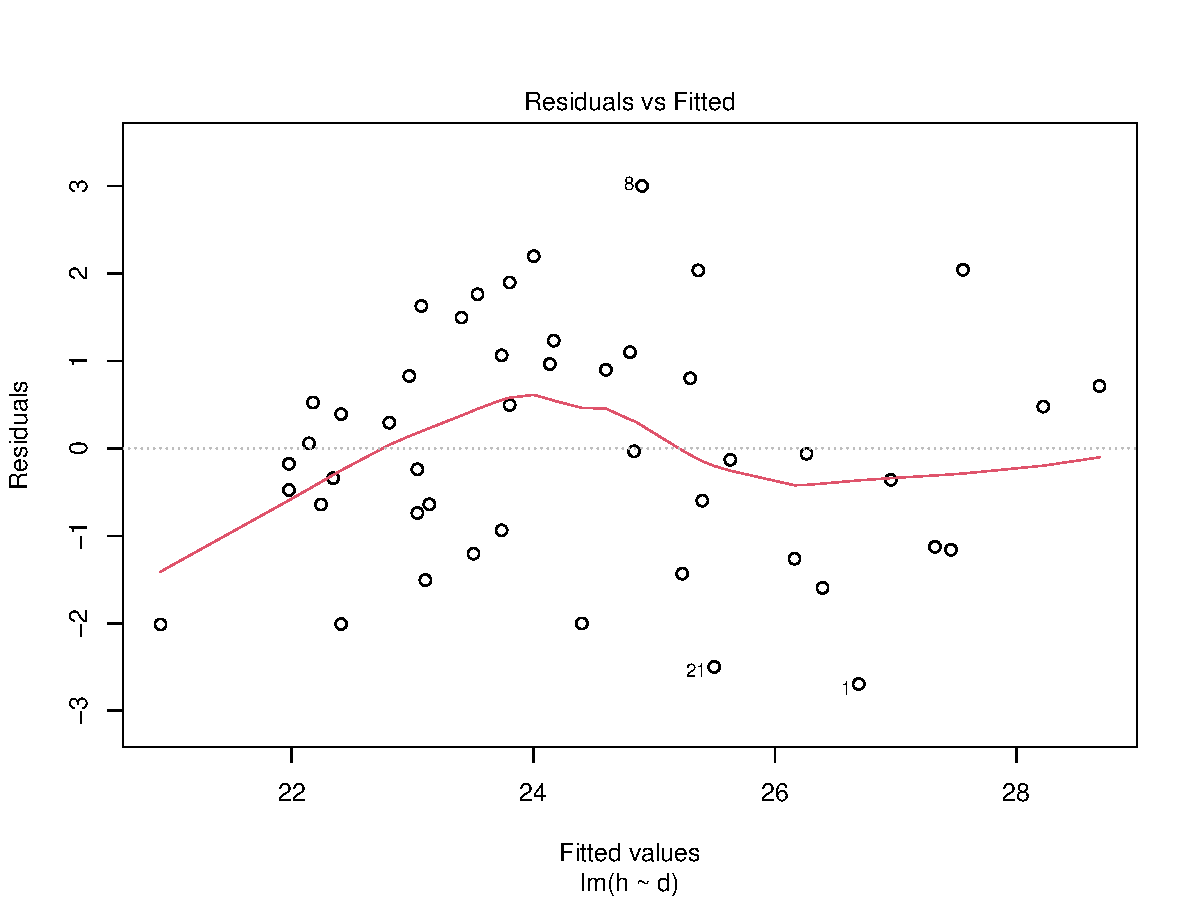
\includegraphics[keepaspectratio]{_main_files/figure-latex/unnamed-chunk-63-1.pdf}}

Vaatame väljundit:

\begin{Shaded}
\begin{Highlighting}[]
\FunctionTok{summary}\NormalTok{(lm\_model)}
\end{Highlighting}
\end{Shaded}

\begin{verbatim}
## 
## Call:
## lm(formula = H ~ D1, data = mudelpuud)
## 
## Residuals:
##      Min       1Q   Median       3Q      Max 
## -2,75109 -1,13190 -0,09022  1,01766  2,96592 
## 
## Coefficients:
##             Estimate Std. Error t value Pr(>|t|)    
## (Intercept) 16,21920    0,86199  18,816  < 2e-16 ***
## D1           0,33648    0,03503   9,605 9,31e-13 ***
## ---
## Signif. codes:  0 '***' 0,001 '**' 0,01 '*' 0,05 '.' 0,1 ' ' 1
## 
## Residual standard error: 1,379 on 48 degrees of freedom
## Multiple R-squared:  0,6578, Adjusted R-squared:  0,6506 
## F-statistic: 92,26 on 1 and 48 DF,  p-value: 9,315e-13
\end{verbatim}

Lineaarse regressioonimudeli kokkuvõte sisaldab mitmeid olulisi statistilisi näitajaid, mis aitavad hinnata mudeli sobivust andmetele.

Determinatsioonikordaja, tuntud ka kui \(R^2\) (R-ruut), on statistiline mõõdik, mida kasutatakse lineaarse regressiooni kontekstis, et hinnata, kui suures ulatuses sõltuva muutuja variatsioon on seletatav sõltumatute muutujate abil mudelis. \(R^2\) väärtus varieerub vahemikus 0 kuni 1, kus 0 tähendab, et mudel ei seleta sõltuva muutuja variatsiooni üldse, samas kui 1 tähendab, et mudel seletab sõltuva muutuja variatsiooni täielikult.

\(R^2\) arvutamiseks kasutatakse järgmist valemit:

\[ R^2 = 1 - \frac{\text{SS}_\text{res}}{\text{SS}_\text{tot}} \]

kus:

\begin{itemize}
\tightlist
\item
  \(\text{SS}_\text{res}\) on jääkide ruutude summa (residual sum of squares), mis mõõdab mudeli poolt seletamata variatsiooni.
\item
  \(\text{SS}_\text{tot}\) on kogu variatsiooni ruutude summa (total sum of squares), mis mõõdab sõltuva muutuja variatsiooni võrreldes tema keskmisega.
\end{itemize}

\textbf{Kõrge \(R^2\) väärtus} (lähedane 1-le) näitab, et mudeli poolt seletatav variatsioon on suur, mis tähendab, et mudel sobib andmetele hästi. See viitab sellele, et suur osa sõltuva muutuja variatsioonist on seletatav mudeli sõltumatute muutujatega.

\textbf{Madal \(R^2\) väärtus} (lähedane 0-le) näitab, et mudel seletab sõltuva muutuja variatsioonist väikese osa, mis tähendab, et mudeli sobivus andmetele on kehv. See võib viidata sellele, et mudelis kasutatavad sõltumatud muutujad ei ole sõltuva muutuja variatsiooni seletamisel tõhusad.

Oluline on mõista, et kuigi \(R^2\) on kasulik mõõdik mudeli sobivuse hindamisel, ei tähenda kõrge \(R^2\) automaatselt, et mudel on õige või et sõltumatud muutujad põhjustavad sõltuva muutuja käitumist. Samuti ei pruugi madal \(R^2\) alati tähendada mudeli ebatõhusust, eriti keerukamate või mittelineaarsete suhete puhul. Lisaks tuleks mudeli hindamisel arvesse võtta ka muid tegureid, nagu mudeli tõlgendatavus, sõltumatute muutujate olulisus ja korrigeeritud \(R^2\).

Lineaarse regressiooni \textbf{nihutamata hinnang}, tuntud ka kui korrigeeritud \(R^2\) (inglise keeles ``adjusted \(R^2\)''), on statistiline mõõdik, mida kasutatakse mudeli seletusvõime hindamiseks, võttes arvesse mudeli sõltumatute muutujate arvu. Erinevalt lihtsast \(R^2\)-st, mis mõõdab, kui suur osa sõltuva muutuja variatsioonist on seletatav mudeli abil, arvestab korrigeeritud \(R^2\) mudeli keerukust, arvestab mudeli liigsete sõltumatute muutujate lisamise eest. See on oluline, kuna mudelisse liiga palju muutujaid lisades võib \(R^2\) väärtus eksitavalt tõusta, viidates paremale mudeli sobivusele, kuigi tegelikult võivad lisatud muutujad olla statistiliselt mitteolulised.

Korrigeeritud \(R^2\) arvutatakse järgmise valemi järgi:

\[ R^2_{\text{adj}} = 1 - \left( \frac{(1 - R^2)(n - 1)}{n - k - 1} \right) \]

kus:

\begin{itemize}
\tightlist
\item
  \(R^2\) on mudeli lihtne determinatsioonikoefitsient,
\item
  \(n\) on vaatluste arv,
\item
  \(k\) on sõltumatute muutujate arv mudelis.
\end{itemize}

Valemist nähtub, et \(R^2_{\text{adj}}\) väheneb, kui lisatakse muutujaid, mis ei paranda mudeli seletusvõimet proportsionaalselt nende arvuga. Seega, erinevalt lihtsast \(R^2\)-st, pakub korrigeeritud \(R^2\) ausamat hinnangut mudeli sobivusele, eriti kui võrrelda mudeleid, mis sisaldavad erinevat arvu sõltumatuid muutujaid. Korrigeeritud \(R^2\) on eriti kasulik mudelite võrdlemisel ja mudeli valimisel, aidates vältida ülemudelitamist ja eelistades mudelit, mis annab parima tasakaalu seletusvõime ja keerukuse vahel.

\begin{itemize}
\item
  P-väärtused näitavad, kas sõltumatu muutuja on statistiliselt oluline mudelis. Kui P-väärtus on väiksem kui 0,05, siis võib järeldada, et sõltumatu muutuja mõjutab oluliselt sõltuvat muutujat.
\item
  Regressioonikordaja väärtused annavad teavet sõltumatute muutujate mõju kohta sõltuvale muutujale.
\end{itemize}

Kokkuvõttes aitab väljund mõista, kuidas mudel sobitub andmetega ja millist infot see pakub sõltuvate ja sõltumatute muutujate seoste kohta.

\subsection{Homoskedastilisuse testimine}\label{homoskedastilisuse-testimine}

Homoskedastilisuse ehk veakvoodi püsimise kontrollimine on oluline samm lineaarse regressioonimudeli sobivuse hindamisel. Alljärgnevalt on näide, kuidas kontrollida lineaarse regressioonimudeli homoskedastilisust:

\textbf{Jääkide vs ennustatud väärtused graafik}: Üks lihtsamaid viise homoskedastilisuse hindamiseks on vaadata lineaarse regressioonimudeli residuaalide (veaväärtused) ja ennustatud väärtuste suhet. Ideaalis peaksid residuaalide hajuvus olema ühtlane kõikide ennustatud väärtuste juures. Graafiku kasutamine aitab visuaalselt hinnata, kas veakvoodi eeldus on täidetud.

\begin{Shaded}
\begin{Highlighting}[]
\FunctionTok{plot}\NormalTok{(lm\_model, }\AttributeTok{which=}\DecValTok{1}\NormalTok{, }\AttributeTok{main =} \StringTok{""}\NormalTok{) }
\end{Highlighting}
\end{Shaded}

\begin{figure}
\centering
\pandocbounded{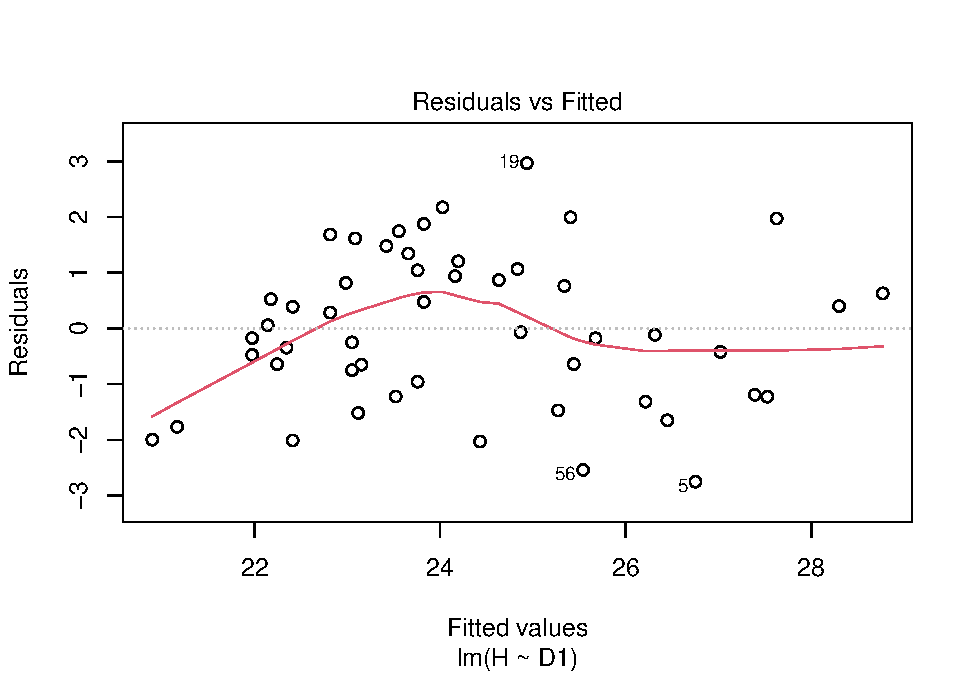
\includegraphics[keepaspectratio]{_main_files/figure-latex/unnamed-chunk-65-1.pdf}}
\caption{\label{fig:unnamed-chunk-65}Jäägid vs ennustatud}
\end{figure}

Lineaarse mudeli homoskedastilisuse testida, võid kasutada ka Breush-Pagan testi või White'i testi. Need testid hindavad, kas residuaalide varieeruvus on seotud sõltumatute muutujatega ning kas see varieeruvus on ühtlane.

\begin{Shaded}
\begin{Highlighting}[]
\NormalTok{lmtest}\SpecialCharTok{::}\FunctionTok{bptest}\NormalTok{(lm\_model)}
\end{Highlighting}
\end{Shaded}

\begin{verbatim}
## 
##  studentized Breusch-Pagan test
## 
## data:  lm_model
## BP = 0,55976, df = 1, p-value = 0,4544
\end{verbatim}

\texttt{lmtest::bptest} testib regressioonimudeli jääkide heteroskedastsuse olemasolu. Heteroskedastsus tähendab, et jääkide varieeruvus ei ole konstantne üle kõigi sõltumatute muutujate väärtuste ning võib tekitada probleeme statistiliste hüpoteeside testimisel.

Testi tulemusi võib lugeda järgmiselt:

\begin{itemize}
\tightlist
\item
  Nullhüpotees (H0): jääkide varieeruvus on konstantne (st heteroskedastsust ei esine).
\item
  Alternatiivhüpotees (H1): jääkide varieeruvus ei ole konstantne (st heteroskedastsus esineb).
\end{itemize}

Testist saadav p-väärtus aitab hinnata, kas on piisavalt tõendeid, et lükata ümber nullhüpotees heteroskedastsuse puudumise kohta. Väike p-väärtus (\textless0,05) viitab sellele, et saame nullhüpoteesi ümber lükata ja järeldada, et heteroskedastsust esineb.

\subsection{Jääkide normaalsuse test}\label{juxe4uxe4kide-normaalsuse-test}

Üks oluline eeldus, mida lineaarses regressioonis kasutatakse, on see, et mudeli jäägid (residuaalid) vastaksid normaaljaotusele. Normaaljaotus tähendab, et andmete jaotus on sümmeetriline ning keskmise jaotusega. Miks on oluline, et lineaarse regressiooni jäägid vastaksid normaaljaotusele?

Parimate tulemuste saamiseks: Kui jäägid on normaaljaotusele lähedased, siis on regressioonimudeli ennustused usaldusväärsemad ja täpsemad.

Statistiliste testide usaldusväärsus: Paljud statistilised testid eeldavad, et andmed vastavad normaaljaotusele. Kui jäägid ei vasta normaaljaotusele, võivad testide tulemused olla ebatäpsed või valed.

Mudeli hindamine: Normaaljaotuse eelduse rikkumine võib viidata sellele, et mudel ei sobi antud andmetele hästi ning on vajalik leida alternatiivseid mudeleid.

Väljendusrikas graafiline analüüs: Normaliseeritud jääkide graafik (residual plot) on üks viis, kuidas hinnata, kas jäägid vastavad normaaljaotusele. See graafik aitab visualiseerida, kas jäägid on juhuslikult hajutatud ümber nulli ja kas nende jaotus on ligilähedane normaaljaotusele.

\begin{Shaded}
\begin{Highlighting}[]
\CommentTok{\# Arvuta mudeli jäägid}
\NormalTok{residuals }\OtherTok{\textless{}{-}} \FunctionTok{residuals}\NormalTok{(lm\_model)}
\end{Highlighting}
\end{Shaded}

Järgmiseks loo qqplot, kasutades arvutatud residuaale:

\begin{Shaded}
\begin{Highlighting}[]
\CommentTok{\# Loome qqploti}
\FunctionTok{qqnorm}\NormalTok{(residuals)}
\FunctionTok{qqline}\NormalTok{(residuals)}
\end{Highlighting}
\end{Shaded}

\pandocbounded{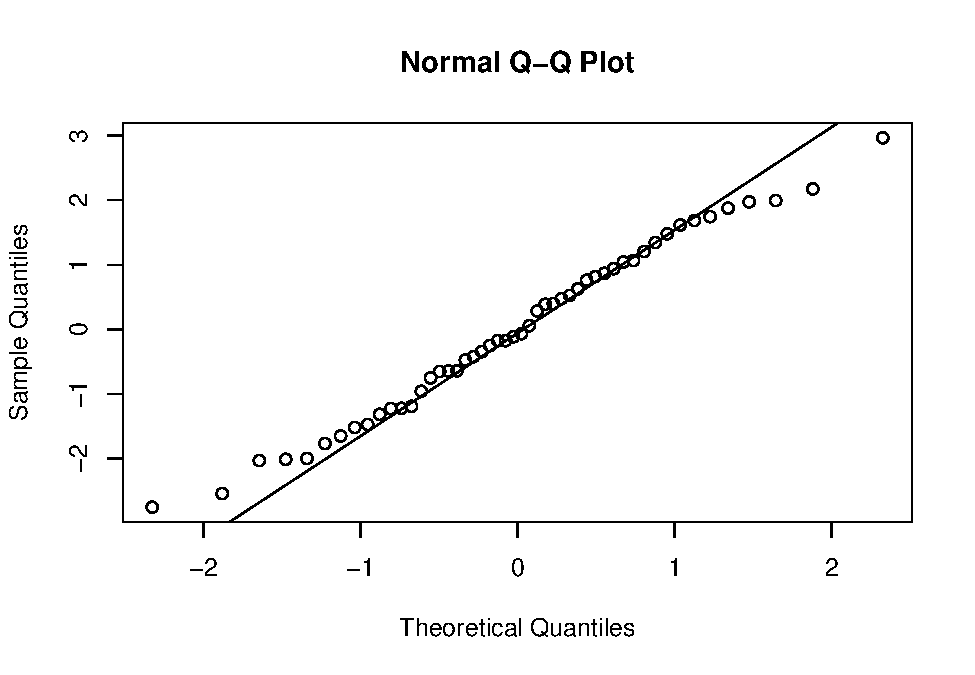
\includegraphics[keepaspectratio]{_main_files/figure-latex/unnamed-chunk-68-1.pdf}}

Samuti saab vaadata jääkide jagunemist tihedusfunktsiooni abil koostatud graafikul.

\begin{Shaded}
\begin{Highlighting}[]
\CommentTok{\# Jääkide jaouts}
\FunctionTok{plot}\NormalTok{(}\FunctionTok{density}\NormalTok{(residuals), }\AttributeTok{main =} \StringTok{""}\NormalTok{)}
\end{Highlighting}
\end{Shaded}

\begin{figure}
\centering
\pandocbounded{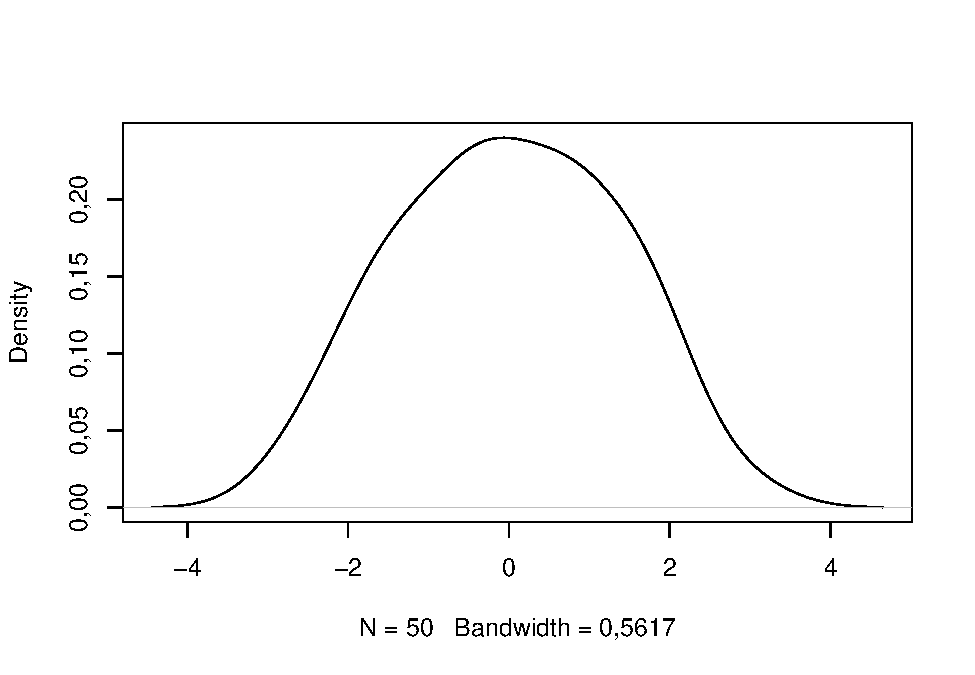
\includegraphics[keepaspectratio]{_main_files/figure-latex/unnamed-chunk-69-1.pdf}}
\caption{\label{fig:unnamed-chunk-69}Jääkide tihedusfunktsioon}
\end{figure}

Kui kõik on korrektselt tehtud, siis peaksid residuaalidest koostatud qq-ploti punktid paiknema peaaegu ideaalselt joone lähedal, mis näitab, et residuaalide jaotus on normaalne.

Sellise protseduuri abil saad hinnata, kui hästi sobib loodud lineaarne regressioonimudel sinu andmetele ning kas residuaalide jaotus vastab normaalsuse eeldusele.

\begin{Shaded}
\begin{Highlighting}[]
\CommentTok{\# ANOVA}
\FunctionTok{anova}\NormalTok{(lm\_model)}
\end{Highlighting}
\end{Shaded}

\begin{verbatim}
## Analysis of Variance Table
## 
## Response: H
##           Df  Sum Sq Mean Sq F value    Pr(>F)    
## D1         1 175,406 175,406  92,257 9,315e-13 ***
## Residuals 48  91,261   1,901                      
## ---
## Signif. codes:  0 '***' 0,001 '**' 0,01 '*' 0,05 '.' 0,1 ' ' 1
\end{verbatim}

\begin{Shaded}
\begin{Highlighting}[]
\FunctionTok{confint}\NormalTok{(lm\_model)}
\end{Highlighting}
\end{Shaded}

\begin{verbatim}
##                  2,5 %    97,5 %
## (Intercept) 14,4860581 17,952339
## D1           0,2660461  0,406918
\end{verbatim}

R-is on võimalik lihtalt lisada mudelisse täiendavad tunnuseid, mis arvutakse mudeli arvutamise käigus. Järgnevas näites on lisatud täiendav tingimus, kas puuliik on mänd (I(PL == ``MA'')).

\begin{Shaded}
\begin{Highlighting}[]
\FunctionTok{summary}\NormalTok{(lm\_model\_pl }\OtherTok{\textless{}{-}} \FunctionTok{lm}\NormalTok{(H }\SpecialCharTok{\textasciitilde{}}\NormalTok{ D1}\SpecialCharTok{+}\FunctionTok{I}\NormalTok{(PL }\SpecialCharTok{==} \StringTok{"MA"}\NormalTok{), }\AttributeTok{data =}\NormalTok{ mudelpuud))}
\end{Highlighting}
\end{Shaded}

\begin{verbatim}
## 
## Call:
## lm(formula = H ~ D1 + I(PL == "MA"), data = mudelpuud)
## 
## Residuals:
##     Min      1Q  Median      3Q     Max 
## -2,2692 -0,8618 -0,1132  0,8078  3,5883 
## 
## Coefficients:
##                   Estimate Std. Error t value Pr(>|t|)    
## (Intercept)       15,85715    0,85115  18,630  < 2e-16 ***
## D1                 0,36250    0,03609  10,046 2,76e-13 ***
## I(PL == "MA")TRUE -0,93425    0,44736  -2,088   0,0422 *  
## ---
## Signif. codes:  0 '***' 0,001 '**' 0,01 '*' 0,05 '.' 0,1 ' ' 1
## 
## Residual standard error: 1,333 on 47 degrees of freedom
## Multiple R-squared:  0,6868, Adjusted R-squared:  0,6735 
## F-statistic: 51,54 on 2 and 47 DF,  p-value: 1,415e-12
\end{verbatim}

Antud juhul on näha, et mänd on teistest statistiliselt oluliselt erinev.

Kui aga vaadata, milline on mudelis kasutatava andmestiku esimesed read. Selles on näha, et uus arvutatud tunnus omab väärtusi TRUE ja FALSE ehk arvutamisel on need vastavalt 1 ja 0.

\begin{Shaded}
\begin{Highlighting}[]
\FunctionTok{head}\NormalTok{(lm\_model\_pl}\SpecialCharTok{$}\NormalTok{model)}
\end{Highlighting}
\end{Shaded}

\begin{verbatim}
##       H   D1 I(PL == "MA")
## 5  24,0 31,3          TRUE
## 7  22,8 22,4         FALSE
## 10 20,4 18,4         FALSE
## 11 25,1 23,6         FALSE
## 12 24,8 27,4          TRUE
## 14 22,3 21,7         FALSE
\end{verbatim}

Samasugust lähenemist on võimalik kasutada ka MS Exceli keskkonnas. Kui me soovime mingi tunnuse taseme kohta saada täpsemalt infot, siis tuleb esmalt luua uus tunnus väärtusega 0 või 1. Näiteks, võtame samad andmed MS Excelis ning lisame tunnuse OnMänd, mille väärtus on 1, kui antud puu on mänd, vastasel juhul on 0.

MS Exceli keskkonnas saab lineaarset regressiooni teha Analysis Toolpak moodulis oleva Regression protseduuriga.

\begin{table}[H]
\caption{Lineaarse regressiooni tulemus MS Exceli keskkonnas.}
\begin{tabular}{r|r|r|r|r|r|r}
\hline
Regression Statistics & & & & & & \\
\hline
Multiple R & 0,829 & & & & & \\
\hline
R Square & 0,687 & & & & & \\
\hline
Adjusted R Square & 0,674 & & & & & \\
\hline
Standard Error & 1,333 & & & & & \\
\hline
Observations & 50 & & & & & \\
\hline
 & & & & & & \\
\hline
ANOVA & & & & & & \\
\hline
 & df & SS & MS & F & Significance F & \\
\hline
Regression & 2 & 183,155 & 91,578 & 51,539 & 0,000 & \\
\hline
Residual & 47 & 83,512 & 1,777 & & & \\
\hline
Total & 49 & 266,667 & & & & \\
\hline
 & & & & & & \\
\hline
 & Coefficients & Standard Error & t Stat & P-value & Lower 95\% & Upper 95\%\\
\hline
Intercept & 15,857 & 0,851 & 18,630 & 0,000 & 14,145 & 17,569\\
\hline
D & 0,363 & 0,036 & 10,046 & 0,000 & 0,290 & 0,435\\
\hline
OnMänd & -0,934 & 0,447 & -2,088 & 0,042 & -1,834 & -0,034\\
\hline
\end{tabular}
\end{table}

\subsection{Multikollineaarsus}\label{multikollineaarsus}

Lineaarses regressioonis tähistab multikolineaarsus olukorda, kus kaks või enam sõltumatut muutujat (selgitajat) on omavahel tugevalt seotud või korreleerunud. See tähendab, et ühe selgitaja väärtusi saab suure täpsusega ennustada teiste selgitajate väärtuste põhjal. Multikolineaarsus võib olla probleemiks, sest:

Mõjutab koefitsientide hinnangute täpsust: multikolineaarsus suurendab koefitsientide hinnangute varieeruvust, mis muudab need ebastabiilseks. Väiksed muudatused andmestikus võivad tuua kaasa suuri muutusi koefitsientide hinnangutes, muutes mudeli interpretatsiooni keeruliseks.

Raskendab muutujate tähtsuse hindamist: kõrge multikollineaarsuse korral võib olla raske kindlaks teha, milline sõltumatu muutuja mõjutab sõltuvat muutujat, sest statistilised testid ei pruugi olla usaldusväärsed. See võib viia oluliste muutujate ebaõiglase kõrvalejätmiseni või ebaoluliste muutujate mudelisse lisamiseni.

Vähendab mudeli interpretatsiooni selgust: kui sõltumatud muutujad on omavahel tugevalt seotud, muutub mudeli interpretatsioon keerulisemaks, kuna keeruline on eristada iga muutuja unikaalset mõju sõltuvale muutujale.

Multikollineaarsuse tuvastamiseks lineaarses regressioonis kasutatakse tavaliselt järgmisi meetodeid:

\begin{itemize}
\tightlist
\item
  \textbf{Korrelatsioonimatriks}: Vaadeldakse sõltumatute muutujate vahelisi korrelatsioonikoefitsiente. Kõrge korrelatsioon näitab võimalikku multikollineaarsust.
\item
  \textbf{Variance Inflation Factor (VIF)}: VIF mõõdab, kui palju muutuja variatiivsus suureneb multikollineaarsuse tõttu. Tavaliselt peetakse VIF väärtust üle 5 või 10 viitavaks tugevale multikollineaarsusele.
\item
  \textbf{Tolerants}: Tolerants on VIF-i pöördväärtus ja näitab, kui suur osa muutuja variatsioonist ei ole seletatav teiste mudeli muutujatega. Madal tolerants viitab multikollineaarsusele.
\end{itemize}

Multikollineaarsuse lahendamiseks võib kasutada mitmeid lähenemisviise, näiteks muutujate eemaldamist mudelist, muutujate kombineerimist või andmete transformeerimist. Samuti võib kasulikuks osutuda regulaarimismeetodite, nagu ridge regressioon või lasso regressioon, kasutamine, mis aitavad vähendada koefitsientide varieeruvust, karistades suuri koefitsiente.

Vaatame järgmist näidet, kus puude kõrgust ennustame mõlema diameetri alusel. Kui varasemalt oli näha, et üks diameeter on oluline, siis antud mudelid ei ole enam kumbki oluline, sest nende tunnuse vahel on korrelatsioon.

\begin{Shaded}
\begin{Highlighting}[]
\FunctionTok{summary}\NormalTok{(lm.col }\OtherTok{\textless{}{-}} \FunctionTok{lm}\NormalTok{(H }\SpecialCharTok{\textasciitilde{}}\NormalTok{ D1 }\SpecialCharTok{+}\NormalTok{ D2, }\AttributeTok{data =}\NormalTok{ mudelpuud))}
\end{Highlighting}
\end{Shaded}

\begin{verbatim}
## 
## Call:
## lm(formula = H ~ D1 + D2, data = mudelpuud)
## 
## Residuals:
##     Min      1Q  Median      3Q     Max 
## -2,7643 -0,8498 -0,1563  0,7700  3,1419 
## 
## Coefficients:
##             Estimate Std. Error t value Pr(>|t|)    
## (Intercept) 15,95391    0,85902  18,572   <2e-16 ***
## D1          -0,05203    0,22886  -0,227   0,8211    
## D2           0,40125    0,23369   1,717   0,0926 .  
## ---
## Signif. codes:  0 '***' 0,001 '**' 0,01 '*' 0,05 '.' 0,1 ' ' 1
## 
## Residual standard error: 1,352 on 47 degrees of freedom
## Multiple R-squared:  0,678,  Adjusted R-squared:  0,6643 
## F-statistic: 49,48 on 2 and 47 DF,  p-value: 2,726e-12
\end{verbatim}

Tehes täiendavalt ANOVA, on näha, et D1, mis lineaarses regressioonis ei olnud oluline, on dispersioonanalüüsi järgi peamine varieeruvuse kirjeldaja.

\begin{Shaded}
\begin{Highlighting}[]
\FunctionTok{anova}\NormalTok{(lm.col)}
\end{Highlighting}
\end{Shaded}

\begin{verbatim}
## Analysis of Variance Table
## 
## Response: H
##           Df  Sum Sq Mean Sq F value    Pr(>F)    
## D1         1 175,406 175,406 96,0019 6,161e-13 ***
## D2         1   5,387   5,387  2,9482   0,09255 .  
## Residuals 47  85,874   1,827                      
## ---
## Signif. codes:  0 '***' 0,001 '**' 0,01 '*' 0,05 '.' 0,1 ' ' 1
\end{verbatim}

\begin{Shaded}
\begin{Highlighting}[]
\FunctionTok{require}\NormalTok{(car)}
\end{Highlighting}
\end{Shaded}

\begin{verbatim}
## Loading required package: car
\end{verbatim}

\begin{verbatim}
## Loading required package: carData
\end{verbatim}

\begin{Shaded}
\begin{Highlighting}[]
\CommentTok{\# Arvutame VIF väärtuse multikollineaarsuse tuvastamiseks}
\FunctionTok{vif}\NormalTok{(lm.col)}
\end{Highlighting}
\end{Shaded}

\begin{verbatim}
##       D1       D2 
## 44,41058 44,41058
\end{verbatim}

Kui VIF väärtus on üle 5, siis on tunnuste vahel tugev korrelatsioon, mida saame kontrollida ka korrelatsioonimaatriksiga.

\begin{Shaded}
\begin{Highlighting}[]
\FunctionTok{cor}\NormalTok{(puud\_data[,}\FunctionTok{c}\NormalTok{(}\StringTok{"D1"}\NormalTok{,}\StringTok{"D2"}\NormalTok{)])}
\end{Highlighting}
\end{Shaded}

\begin{verbatim}
##           D1        D2
## D1 1,0000000 0,9860028
## D2 0,9860028 1,0000000
\end{verbatim}

Sellest on näha, et need on tugevas korrelatsioonis (0,986). See mõjutab ka lineaarse regressiooni parameetrite arvutamist.

\section{Dispersioonanalüüs}\label{dispersioonanaluxfcuxfcs}

Mitmese regressioonanalüüsi korral on tegemist mudeliga, kus pidev funktsioontunnus avaldub pidevate argumenttunnuste lineaarkombinatsioonina. Dispersioonanalüüsi korral on tegemist mudelitega, kus funktsioontunnuseks on pidev tunnus, kuid argument-tunnused on diskreetsed (võivad olla nii arvulised kui ka mittearvulised). Dispersioon-analüüsi argumenttunnuseid nimetatakse faktoriteks. Ühefaktorilise dispersioonanalüüsi puhul uuritakse funktsioontunnuse sõltuvust ainult ühest faktorist. Faktori võimalikke väärtusi nimetatakse faktori tasemeteks.

Olgu üldkogum jaotatud mittelõikuvateks osadeks ehk rühmadeks faktori tasemete järgi. Öeldakse, et faktor X mõjub tunnusele Y, kui tunnuse Y keskväärtused eri rühmades on erinevad. Uurija käsutuses on valimi mõõtmisandmed, mille funktsioon-tunnuse rühmakeskmised tavaliselt erinevad. Dispersioonanalüüs on meetod, millega otsitakse vastust küsimusele, kas valimi rühma¬keskmiste erinevus on põhjustatud uuritava faktori mõjust või valimi juhuslikkusest.

Dispersioonanalüüsi võimalused ja vahendid sõltuvad oluliselt valitud mudelist ja katsekorraldusest. Kui iga faktortunnuse igal tasemel on tehtud ühepalju mõõtmisi, nimetatakse mudelit tasakaalustatuks, vastasel juhul on tegemist tasakaalustamata mudeliga. Kui mõõtmisi on tehtud faktori kõigil võimalikel tasemetel, siis nimetatakse seda fikseeritud faktoriks. Kui faktortunnusel on palju erinevaid väärtusi ja mõõdetud tasemeid vaadeldakse juhusliku valimina faktori võimalike tasemete hulgast, siis nimetatakse seda juhuslikuks faktoriks. Järgnevalt käsitleme ainult fikseeritud faktoritega mudeleid.

\chapter{Mittelineaarne regressioon}\label{mittelineaarne-regressioon}

Mõnikord on vaja funktsioontunnuse sõltuvust argumenttunnusest lähendada funkt-siooniga, mida ei ole võimalik teisendada parameetrite suhtes lineaarsele kujule. Tavaliselt kasutatakse mitte¬lineaarseid funktsioone suhteliselt keeruliste tugevalt kõver-jooneliste sõltuvuste modelleerimiseks. Mudelina rakendatavad funktsioonid on mitte-lineaarsed seetõttu, et nad on tuletatud modelleeritava protsessi olemust kajas¬tavatest eeldustest.
Mittelineaarse regressioonivalemi parameetrite hindamine katseandmete põhjal on üsna problemaatiline ülesanne. Selleks peab funktsiooni parameetrite kohta teadma nende ligikaudseid alghinnanguid. Mittelineaarsete parameetrite hindamiseks tuleb kasutada mingit optimeerimis¬algoritmi, mille arvutamine on tunduvalt aeganõudvam, kui lineaarse regressioonanalüüsi tegemine. Lisaks sellele ei õnnestugi alati optimaalset lahendit saada.

Näiteks, kui soovime R-is kasutada \texttt{nls()} mudelit, mis kirjeldab puu kõrgust sõltuvalt puu diameetrist, võime kasutada järgmist näidiskoodi.

\begin{Shaded}
\begin{Highlighting}[]
\CommentTok{\# Loe andmed sisse failist "puud.xlsx"}
\NormalTok{andmed }\OtherTok{\textless{}{-}} \FunctionTok{subset}\NormalTok{(openxlsx}\SpecialCharTok{::}\FunctionTok{read.xlsx}\NormalTok{(}\StringTok{"data/puud.xlsx"}\NormalTok{), H }\SpecialCharTok{\textgreater{}} \DecValTok{0}\NormalTok{)}

\CommentTok{\# Määratle mudeli funktsioon}
\NormalTok{puu\_mudel }\OtherTok{\textless{}{-}} \ControlFlowTok{function}\NormalTok{(D, a, b, c) \{}
 \FloatTok{1.3} \SpecialCharTok{+}\NormalTok{ a }\SpecialCharTok{*}\NormalTok{ (D }\SpecialCharTok{/}\NormalTok{ (D }\SpecialCharTok{+}\NormalTok{ b))}\SpecialCharTok{\^{}}\NormalTok{c}
\NormalTok{\}}

\CommentTok{\# Omista algväärtused parameetritele}
\NormalTok{algväärtused }\OtherTok{\textless{}{-}} \FunctionTok{list}\NormalTok{(}\AttributeTok{a =} \DecValTok{1}\NormalTok{, }\AttributeTok{c =} \FloatTok{0.5}\NormalTok{)}

\CommentTok{\# Sobita mudel andmetele}
\NormalTok{mudel }\OtherTok{\textless{}{-}} \FunctionTok{nls}\NormalTok{(H }\SpecialCharTok{\textasciitilde{}} \FunctionTok{puu\_mudel}\NormalTok{(D1, a, }\DecValTok{5}\NormalTok{, c), }\AttributeTok{data =}\NormalTok{ andmed, }\AttributeTok{start =}\NormalTok{ algväärtused)}

\CommentTok{\# Vaata mudeli kokkuvõtet}
\FunctionTok{summary}\NormalTok{(mudel)}
\end{Highlighting}
\end{Shaded}

\begin{verbatim}
## 
## Formula: H ~ puu_mudel(D1, a, 5, c)
## 
## Parameters:
##   Estimate Std. Error t value Pr(>|t|)    
## a  34,3630     1,3616   25,24  < 2e-16 ***
## c   2,0495     0,2029   10,10 1,81e-13 ***
## ---
## Signif. codes:  0 '***' 0,001 '**' 0,01 '*' 0,05 '.' 0,1 ' ' 1
## 
## Residual standard error: 1,316 on 48 degrees of freedom
## 
## Number of iterations to convergence: 7 
## Achieved convergence tolerance: 2,429e-06
\end{verbatim}

Esitame selle kohta ka graafiku, millele lisame mudeli joone funktsioonidega \texttt{curve()} ja \texttt{predict()}, milles kasutame loodud mudeli objekti.

\begin{Shaded}
\begin{Highlighting}[]
\FunctionTok{plot}\NormalTok{(H}\SpecialCharTok{\textasciitilde{}}\NormalTok{D1, andmed, }\AttributeTok{ylim=}\FunctionTok{c}\NormalTok{(}\DecValTok{10}\NormalTok{, }\DecValTok{35}\NormalTok{), }\AttributeTok{xlim =} \FunctionTok{c}\NormalTok{(}\DecValTok{10}\NormalTok{, }\DecValTok{40}\NormalTok{))}
\FunctionTok{curve}\NormalTok{(}\FunctionTok{predict}\NormalTok{(mudel, }\FunctionTok{data.frame}\NormalTok{(}\AttributeTok{D1 =}\NormalTok{ x)), }\DecValTok{10}\NormalTok{, }\DecValTok{40}\NormalTok{, }\AttributeTok{add=}\NormalTok{T, }\AttributeTok{col =} \DecValTok{2}\NormalTok{)}
\end{Highlighting}
\end{Shaded}

\begin{figure}
\centering
\pandocbounded{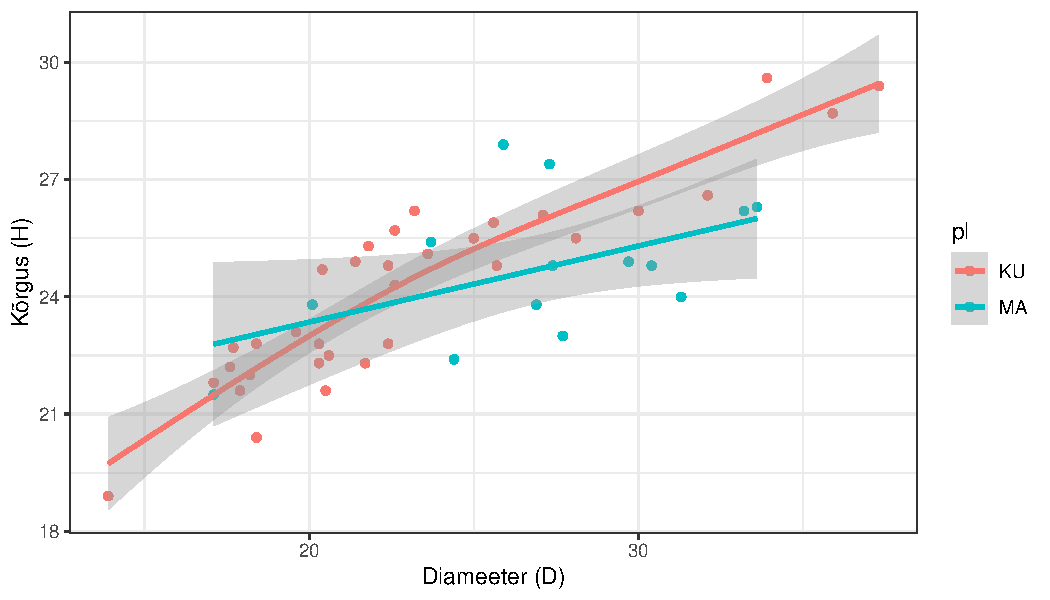
\includegraphics[keepaspectratio]{_main_files/figure-latex/unnamed-chunk-78-1.pdf}}
\caption{\label{fig:unnamed-chunk-78}Mittelineaarne regressioon}
\end{figure}

Kontrollime

\begin{Shaded}
\begin{Highlighting}[]
\FunctionTok{plot}\NormalTok{(}\FunctionTok{fitted}\NormalTok{(mudel), }\FunctionTok{resid}\NormalTok{(mudel),}
 \AttributeTok{xlab =} \StringTok{"Ennustatud väärtused"}\NormalTok{,}
 \AttributeTok{ylab =} \StringTok{"Jäägid"}
\NormalTok{ )}
\FunctionTok{abline}\NormalTok{(}\AttributeTok{h =} \DecValTok{0}\NormalTok{, }\AttributeTok{col =} \StringTok{"red"}\NormalTok{)}
\end{Highlighting}
\end{Shaded}

\begin{figure}
\centering
\pandocbounded{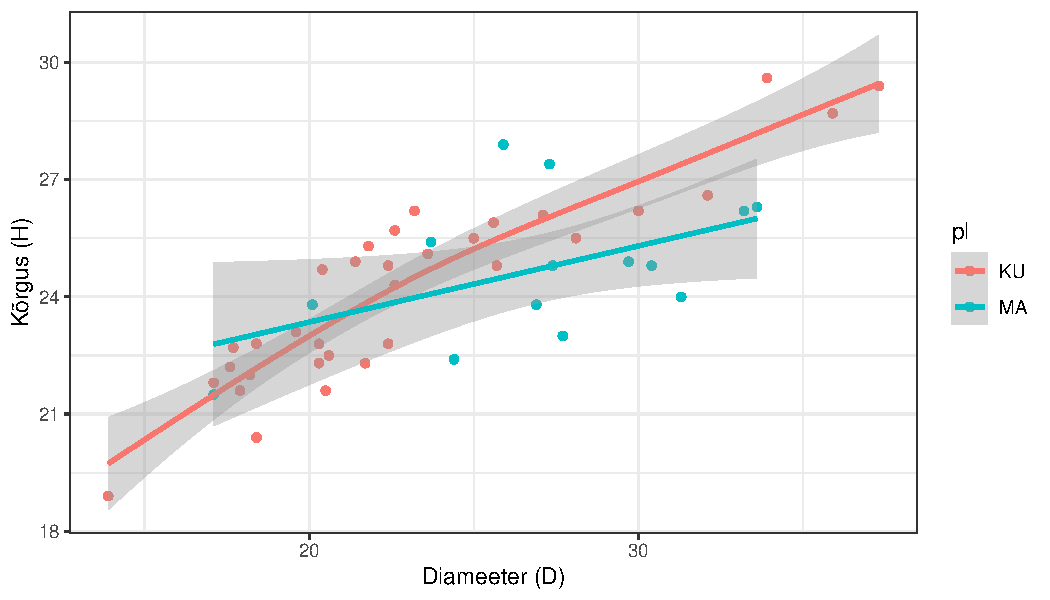
\includegraphics[keepaspectratio]{_main_files/figure-latex/unnamed-chunk-79-1.pdf}}
\caption{\label{fig:unnamed-chunk-79}Jäägid vs ennustatud}
\end{figure}

\begin{Shaded}
\begin{Highlighting}[]
\FunctionTok{qqnorm}\NormalTok{(}\FunctionTok{resid}\NormalTok{(mudel), }\AttributeTok{main =} \StringTok{""}\NormalTok{)}
\FunctionTok{qqline}\NormalTok{(}\FunctionTok{resid}\NormalTok{(mudel), }\AttributeTok{col =} \StringTok{"red"}\NormalTok{)}
\end{Highlighting}
\end{Shaded}

\begin{figure}
\centering
\pandocbounded{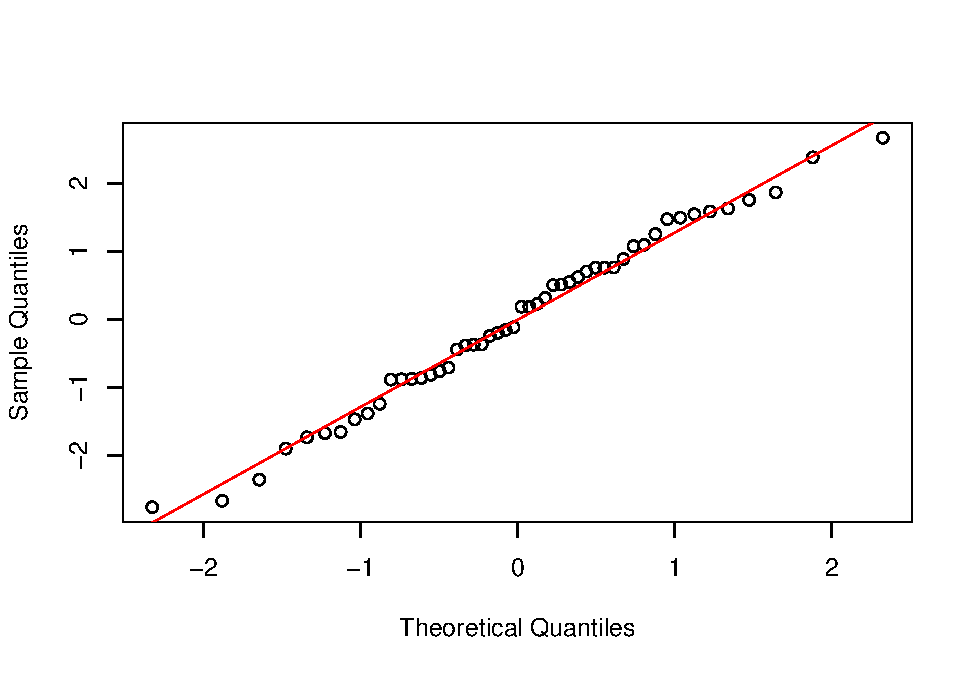
\includegraphics[keepaspectratio]{_main_files/figure-latex/unnamed-chunk-80-1.pdf}}
\caption{\label{fig:unnamed-chunk-80}Jääkide normaaljaotuse test}
\end{figure}

MS Exceli keskkonnas saab mittelineaarse funktsiooni parameetrite hindamiseks kasutada optimeerimisprotseduuri Solver. Selleks tuleks MS Exceli töölehele salvestada argumenttunnuse väärtused, funktsioontunnuse väärtused, prognoosifunktsiooni arvutusvalemid ja prognoosijääkide ruutude summa arvutuseeskiri. Samuti peavad töölehel olema lahtrid funktsiooni parameetrite jaoks, mida prognoosifunktsiooni arvutusvalemid kasutavad.

\chapter{Mitteparameetriline analüüs}\label{mitteparameetriline-analuxfcuxfcs}

\section{Üldistatud aditiivne mudel}\label{uxfcldistatud-aditiivne-mudel}

Üldistatud aditiivne mudel (GAM) on statistiline mudel, mis võimaldab üldistatud lineaarsel mudelil rakendada aditiivse mudeli sujuva ülemineku omadusi. See võimaldab modelleerida mitte-lineaarset sõltuvussuhet eesmärgi muutuja ja sellega seotud tunnuste vahel, lisades mudelisse siledaid funktsioone.

GAM mudelit saab R-keskkonnas rakendada package'iga ``mgcv'' (Multidimensional Generalized Cross-Validation) ning see võimaldab kasutajal määrata siledad funktsioonid (nt splines, loess), mis kajastavad eesmärgi muutuja ja sellega seotud tunnuste vahelist mitte-lineaarset seost.

GAM mudeli loomisel tuleb määrata eesmärgi muutuja ning sellega seotud tunnused, mida soovitakse mudelis arvesse võtta. Samuti tuleb valida siledad funktsioonid ja kontrollida, kas mudel on piisavalt hea eesmärgi või nähtuse seletamiseks. Mudeli sobivuse hindamiseks saab kasutada erinevaid meetodeid, nagu näiteks R-ruut (R-squared) või ristvaliatsioon.

Kokkuvõttes võimaldab GAM mudel R-keskkonnas paindlikult modelleerida mitte-lineaarseid seoseid andmete vahel ning anda sügavamat arusaamist analüüsitava nähtuse kohta.

GAM mudel on statistiline meetod, mis võimaldab mittemeetriliste muutujate mitte-lineaarset mõju modelleerimist. Allpool on näide GAM mudeli kasutamisest R-i tarkvaras:

Järgnevalt demonstreerime, kuidas kasutada üldistatud aditiivset mudelit (GAM) sõltuva muutuja \(H\) ja sõltumatu muutuja \(D1\) suhte modelleerimiseks, kasutades andmestikku \texttt{andmed}. Seejärel visualiseeritakse andmed ja mudeli ennustused.

\begin{Shaded}
\begin{Highlighting}[]
\FunctionTok{require}\NormalTok{(mgcv)}
\end{Highlighting}
\end{Shaded}

\begin{verbatim}
## Loading required package: mgcv
\end{verbatim}

\begin{verbatim}
## Loading required package: nlme
\end{verbatim}

\begin{verbatim}
## This is mgcv 1.9-1. For overview type 'help("mgcv-package")'.
\end{verbatim}

\begin{itemize}
\tightlist
\item
  \textbf{Mudeli loomine kasutades \texttt{gam} funktsiooni:}
\item
  \texttt{gam\_model\ \textless{}-\ gam(H\ \textasciitilde{}\ s(D1),\ data=andmed)}
\item
  See rida loob generaliseeritud aditiivse mudeli, määrates sõltuvaks muutujaks \(H\) ja sõltumatuks muutujaks \(D1\), kasutades sujuvusfunktsiooni \texttt{s()}. Sujuvusfunktsioon võimaldab modelleerida keerukamaid, mittelineaarseid suhteid \(H\) ja \(D1\) vahel. Mudeli loomiseks kasutatakse andmestikku \texttt{andmed}.
\end{itemize}

\begin{Shaded}
\begin{Highlighting}[]
\CommentTok{\# loome GAM mudeli}
\NormalTok{(gam\_model }\OtherTok{\textless{}{-}} \FunctionTok{gam}\NormalTok{(H }\SpecialCharTok{\textasciitilde{}} \FunctionTok{s}\NormalTok{(D1), }\AttributeTok{data=}\NormalTok{andmed))}
\end{Highlighting}
\end{Shaded}

\begin{verbatim}
## 
## Family: gaussian 
## Link function: identity 
## 
## Formula:
## H ~ s(D1)
## 
## Estimated degrees of freedom:
## 3,72  total = 4,72 
## 
## GCV score: 1,680183
\end{verbatim}

\begin{itemize}
\tightlist
\item
  \textbf{Andmete visualiseerimine:}
\item
  \texttt{plot(H\textasciitilde{}D1,\ andmed,\ ylim=c(10,\ 35),\ xlim\ =\ c(10,\ 40))}
\item
  See rida visualiseerib andmed, joonistades \(H\) väärtused sõltuvalt \(D1\) väärtustest, kasutades andmestikku \texttt{andmed}. \texttt{ylim} ja \texttt{xlim} argumendid määravad vastavalt y- ja x-telje piirid, et parandada graafiku loetavust, seades y-telje piirid vahemikku 10 kuni 35 ja x-telje piirid vahemikku 10 kuni 40.
\item
  \texttt{curve(predict(gam\_model,\ data.frame(D1\ =\ x)),\ 10,\ 40,\ add=T,\ col\ =\ 2)}
\item
  See rida lisab esialgsele graafikule mudeli ennustused. \texttt{predict} funktsioon arvutab ennustatud \(H\) väärtused uute \(D1\) väärtuste jaoks, kasutades \texttt{gam\_model} mudelit. \texttt{curve} funktsioon joonistab need ennustused graafikule vahemikus 10 kuni 40, kasutades \texttt{x} kui sõltumatut muutujat, mis esindab \(D1\) väärtusi. \texttt{add=T} argument tähistab, et ennustuskõver lisatakse olemasolevale graafikule, ja \texttt{col\ =\ 2} määrab ennustuskõvera värvi (tavaliselt punane).
\end{itemize}

\begin{Shaded}
\begin{Highlighting}[]
\FunctionTok{plot}\NormalTok{(H}\SpecialCharTok{\textasciitilde{}}\NormalTok{D1, andmed, }\AttributeTok{ylim=}\FunctionTok{c}\NormalTok{(}\DecValTok{10}\NormalTok{, }\DecValTok{35}\NormalTok{), }\AttributeTok{xlim =} \FunctionTok{c}\NormalTok{(}\DecValTok{10}\NormalTok{, }\DecValTok{40}\NormalTok{))}
\FunctionTok{curve}\NormalTok{(}\FunctionTok{predict}\NormalTok{(gam\_model, }\FunctionTok{data.frame}\NormalTok{(}\AttributeTok{D1 =}\NormalTok{ x)), }\DecValTok{10}\NormalTok{, }\DecValTok{40}\NormalTok{, }\AttributeTok{add=}\NormalTok{T, }\AttributeTok{col =} \DecValTok{2}\NormalTok{)}
\end{Highlighting}
\end{Shaded}

\begin{figure}
\centering
\pandocbounded{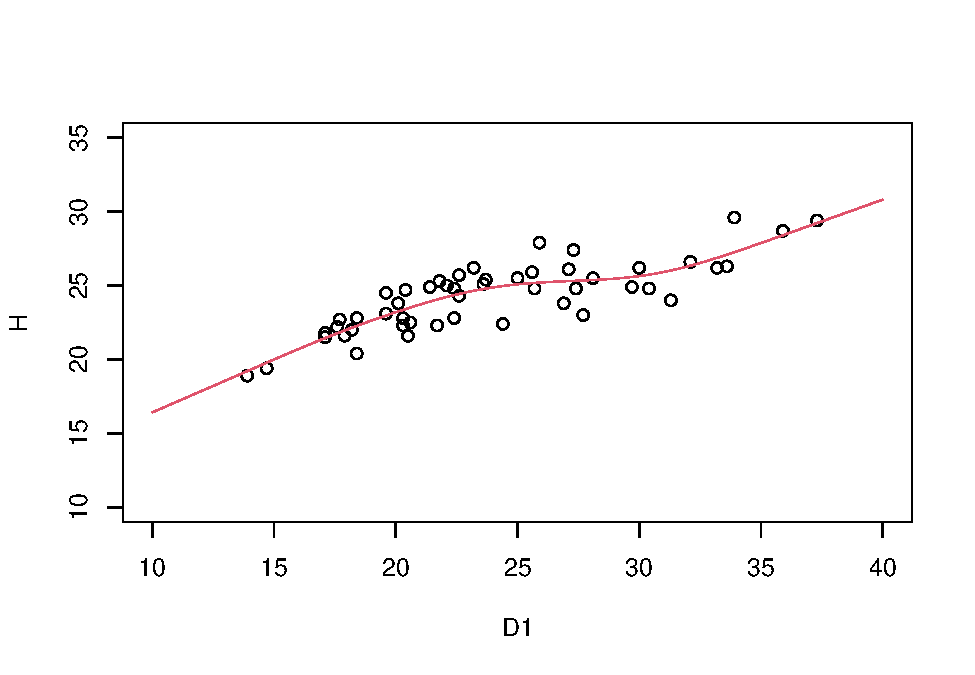
\includegraphics[keepaspectratio]{_main_files/figure-latex/unnamed-chunk-84-1.pdf}}
\caption{\label{fig:unnamed-chunk-84}Üldistatud aditiivse mudel}
\end{figure}

\begin{itemize}
\tightlist
\item
  \textbf{Komponendi sujuvusgraafikud:}
\item
  \texttt{plot(gam\_model)}.
\item
  Kui mudel sisaldab sujuvusfunktsiooni \texttt{s()} kasutades määratletud sõltumatu muutuja \(D1\), genereeritakse sujuvusgraafik, mis näitab, kuidas sõltuv muutuja \(H\) muutub sõltumatu muutuja \(D1\) suhtes. Graafikud illustreerivad sujuva komponendi mõju, koos usaldusvahemikega, mis aitavad hinnata mudeli kindlust ja varieeruvust.
\end{itemize}

\begin{Shaded}
\begin{Highlighting}[]
\FunctionTok{plot}\NormalTok{(gam\_model)}
\end{Highlighting}
\end{Shaded}

\begin{figure}
\centering
\pandocbounded{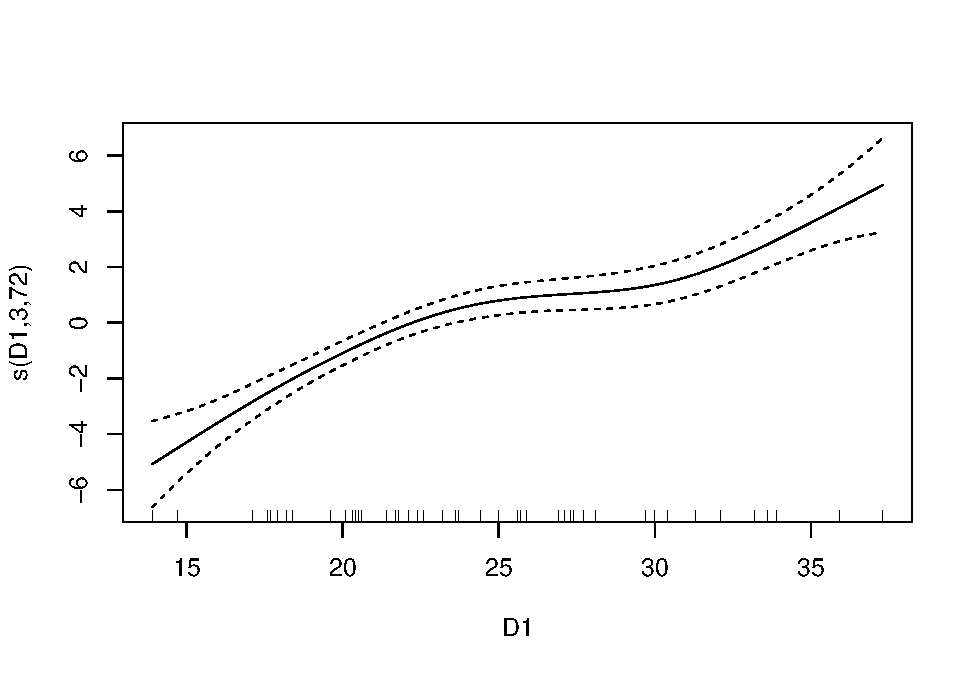
\includegraphics[keepaspectratio]{_main_files/figure-latex/unnamed-chunk-85-1.pdf}}
\caption{\label{fig:unnamed-chunk-85}Üldistatud aditiivse mudeli mõju}
\end{figure}

\begin{itemize}
\item
  \textbf{jääkide tihedusjaotust}
\item
  \texttt{resid(gam\_model)}
\item
  See funktsioon arvutab ja tagastab mudeli \texttt{gam\_model} jäägid, mis on vahe tegelike ja ennustatud väärtuste vahel. Jäägid on olulised mudeli sobivuse ja eelduste kontrollimiseks.
\item
  \texttt{density()}
\item
  Funktsioon arvutab jääkide tihedusfunktsiooni, mis on sujuv hinnang jääkide jaotusele. Tihedusfunktsioon näitab, kui tõenäoline on iga jääkide väärtus, andes visuaalse esituse jääkide jaotusest.
\item
  \texttt{plot()}
\item
  Lõpuks joonistab \texttt{plot} funktsioon tihedusfunktsiooni graafiku. Parameeter \texttt{main\ =\ ""} määrab, et graafikul ei ole pealkirja, jättes graafiku ülaosa tühjaks.
\end{itemize}

\begin{Shaded}
\begin{Highlighting}[]
\FunctionTok{plot}\NormalTok{(}\FunctionTok{density}\NormalTok{(}\FunctionTok{resid}\NormalTok{(gam\_model)), }\AttributeTok{main =} \StringTok{""}\NormalTok{)}
\end{Highlighting}
\end{Shaded}

\begin{figure}
\centering
\pandocbounded{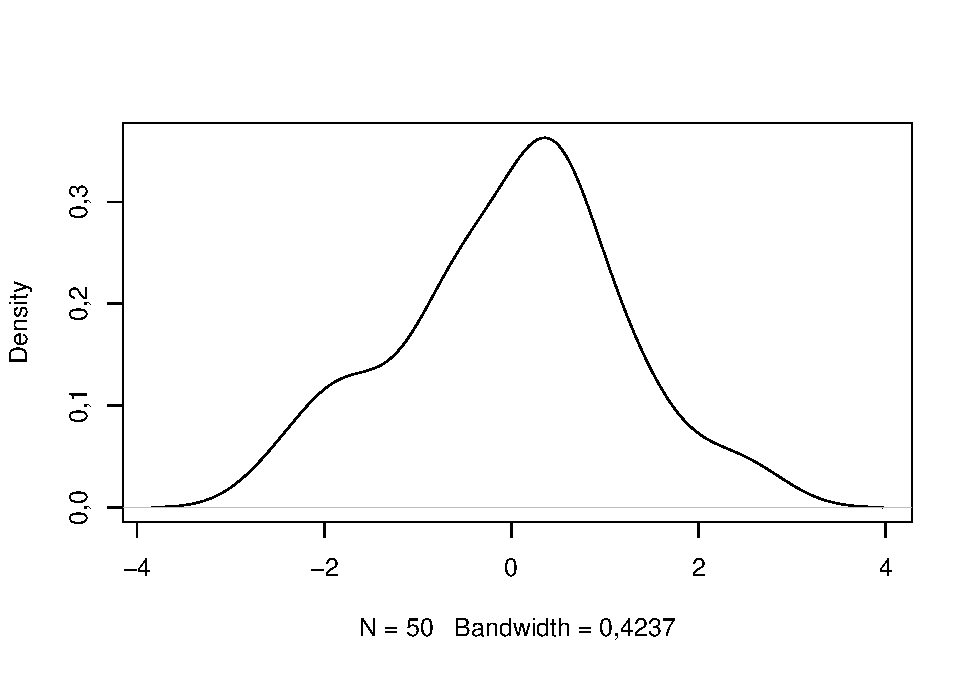
\includegraphics[keepaspectratio]{_main_files/figure-latex/unnamed-chunk-86-1.pdf}}
\caption{\label{fig:unnamed-chunk-86}Jääkide tihedusfunktsioon}
\end{figure}

\bibliography{book.bib,packages.bib}

\end{document}
